\documentclass{tstextbook}

\usepackage{color}
\usepackage{tabularx}
\usepackage{hyperref}
\usepackage{float}
\usepackage[dutch]{babel}
\usepackage{listings}
\definecolor{javared}{rgb}{0.6,0,0} % for strings
\definecolor{javagreen}{rgb}{0.25,0.5,0.35} % comments
\definecolor{javapurple}{rgb}{0.5,0,0.35} % keywords
\definecolor{javadocblue}{rgb}{0.25,0.35,0.75} % javadoc
\usepackage{pgffor, ifthen}
\usepackage{enumitem}
\newcommand{\notes}[3][\empty]{%
    \noindent Notes\vspace{10pt}\\
    \foreach \n in {1,...,#2}{%
        \ifthenelse{\equal{#1}{\empty}}
            {\rule{#3}{0.5pt}\\}
            {\rule{#3}{0.5pt}\vspace{#1}\\}
        }
}
 
\lstset{
  basicstyle=\footnotesize\tt,        % the size of the fonts that are used for the code
  breakatwhitespace=false,         % sets if automatic breaks should only happen at whitespace
  breaklines=true,                 % sets automatic line breaking
  captionpos=b,                    % sets the caption-position to bottom
  extendedchars=true,              % lets you use non-ASCII characters; for 8-bits encodings only, does not work with UTF-8
  frame=single,                    % adds a frame around the code
  language=Java,                 % the language of the code
  showspaces=false,                % show spaces everywhere adding particular underscores; it overrides 'showstringspaces'
  showstringspaces=false,          % underline spaces within strings only
  showtabs=false,                  % show tabs within strings adding particular underscores
  tabsize=2,                      % sets default tabsize to 2 spaces
  keywordstyle=\color{javapurple}\bfseries,
 stringstyle=\color{javared},
 commentstyle=\color{javagreen},
 morecomment=[s][\color{javadocblue}]{/**}{*/},
}

\newtheorem{envoefening}{Oefening}[chapter]
\newenvironment{oefening}
               {\begin{boxexercise}\begin{envoefening}}
               {\end{envoefening}\end{boxexercise}}
               

\begin{document}

\tsbook{Java Advanced 2022-2023}
       {Nele Custers}
       {nvt}
       {2022-2023}
       {xxxxx}{xxx--xx--xxxx--xx--x}{0.0}
       {Hogeschool PXL}
       {Hasselt}
       
\pagebreak

%---------------------------------------------------------------------------
% Chapters
%---------------------------------------------------------------------------

%---------------------------------------------------------------------------

\chapter{Herhaling}

\begin{summary}
Voor de meesten is het alweer even geleden dat je de Java ontwikkelomgeving nog gebruikte. Daarom starten we met een korte herhaling zodat je weer weet hoe je een klasse, interface en enum in Java implementeert en je de syntax van Java weer helemaal in de vingers krijgt. Ook zorgen we ervoor dat je zeker terug bekend bent met het concept polymorfisme. In dit eerste hoofdstuk implementeer je een aantal klassen voor een streaming service (zoals Streamz of Netflix). Deze streaming service zullen we tijdens de komende weken uitbreiden als we nieuwe mogelijkheden van de JDK (Java Development Kit) ontdekken. 
\end{summary}

\section{Klasse}
Java is een object-geori\"enteerde programmeertaal. In een Java programma ga je  objecten aanmaken die je dan gaat manipuleren.
Het is in een klasse dat je het bouwplan of de blueprint voor de objecten definieert. In de klasse beschrijf je alle eigenschappen en het gedrag (de methoden) die gemeenschappelijk zijn voor alle objecten van \'e\'en type.

We starten met een eenvoudige klasse Movie. In deze klasse beschrijven we dat iedere film de volgende eigenschappen heeft:
\begin{itemize}
\item een titel (title)
\item een regisseur (director): voorlopig houden we enkel zijn of haar naam bij in een eigenschap met datatype String
\item een releasedatum (releaseDate)
\item de duur (duration): we gaan de duur van de film bijhouden in minuten
\end{itemize}

\begin{lstlisting}
import java.time.LocalDate;

public class Movie { 
	public static final int LONG_PLAYING_TIME = 2 * 60 + 15;

	private String title;
	private String director;
	private LocalDate releaseDate;
	private int duration;

	public Movie(String title) {
		this.title = title;
	}

	public String getTitle() {
		return title;
	}

	public void setTitle(String title) {
		this.title = title;
	}

	public String getDirector() {
		return director;
	}

	public void setDirector(String director) {
		this.director = director;
	}

	public LocalDate getReleaseDate() {
		return releaseDate;
	}

	public void setReleaseDate(LocalDate releaseDate) {
		this.releaseDate = releaseDate;
	}

	public int getDuration() {
		return duration;
	}

	public void setDuration(int duration) {
		this.duration = duration;
	}
	
	public boolean isLongPlayingTime() {
		return duration > LONG_PLAYING_TIME;
	}

	@Override
	public String toString() {
		return title;
	}
}
\end{lstlisting}

Na de oplijsting van de eigenschappen zie je de \textbf{constructor} van de klasse Movie. Als je in een programma dus een Movie-object aanmaakt moet je steeds een titel opgeven.
De eigenschappen director en releaseDate hebben dus na het aanmaken van het object nog geen waarde, ze hebben de waarde \emph{null} tot het ogenblik dat er via de \emph{setter} een waarde wordt toegekend.

\begin{figure}
  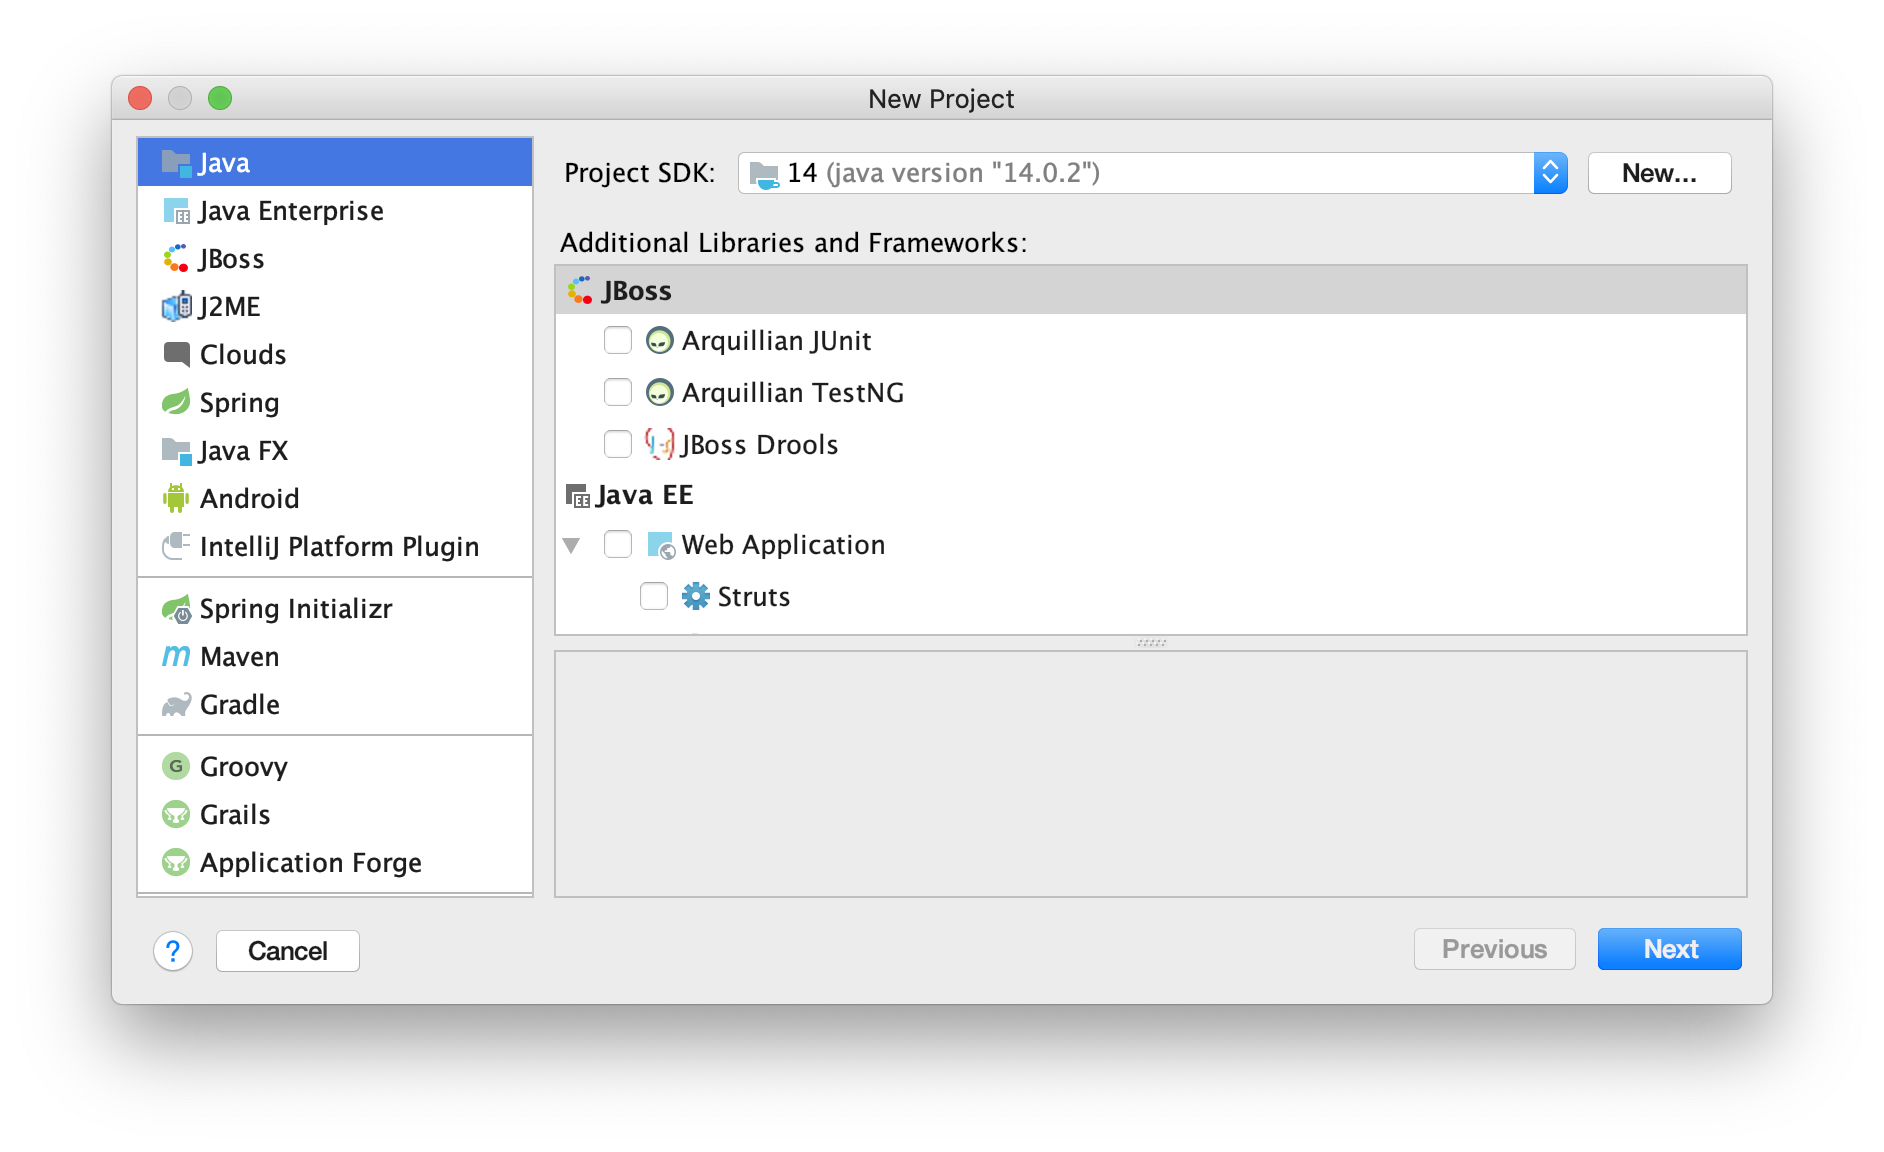
\includegraphics[width=\linewidth]{images/h1/new_java_project.png}
  \caption{Nieuw project aanmaken}
  \label{fig:new_project}
\end{figure}

\begin{oefening}
Open de Java ontwikkelomgeving IntelliJ IDEA en maak een nieuw project aan zoals getoond in figuur \ref{fig:new_project}. Zorg er eveneens voor dat je \textbf{JDK 17} hebt ge\"installeerd. 
Voorzie een package be.pxl.ja.opdracht1. In dit package implementeer je de bovenstaande klasse Movie. Welke code kan je door de ontwikkelomgeving laten genereren?
\begin{itemize}
\item Voorzie een hoofdprogramma waarin je 2 objecten van de klasse Movie aanmaakt.
\item Geef de eigenschap director van 1 van de films een waarde door gebruik te maken van de setter.
\item Toon de waarde van de eigenschap director in de console.
\item Pas de methode \emph{toString()} aan zodat naast de titel van de film ook het jaar (enkel het jaar!) wordt weergegeven indien de releaseDate is ingevuld (bijv. Titanic (1997)). Test de toString()-methode uit.
\end{itemize} 
\end{oefening}

\begin{remark}
Neem de tijd om enkele shortcuts van IntelliJ IDEA te leren kennen.\\
\url{https://www.jetbrains.com/help/idea/mastering-keyboard-shortcuts.html}\\
\url{https://www.jrebel.com/blog/intellij-shortcuts}
\end{remark}

\section{Enum}

De \textbf{enum} of \textbf{opsomming} zorgt ervoor dat je de mogelijke waarden van een eigenschap kan beperken.
In onze klasse Movie voegen we nu een extra eigenschap toe: genre. 
We zouden voor deze eigenschap het datatype String kunnen gebruiken,  maar omdat we hier enkel voorgedefinieerde waarden toelaten maken we een enum-klasse Genre.

\begin{lstlisting}
public enum Genre {

	ACTION("Action"),
	ANIMATION("Animation"),
	ADVENTURE("Adventure"),
	COMEDY("Comedy"),
	CRIME("Crime & Gangster", "mdi-fingerprint"),
	DRAMA("Drama"),
	DOCUMENTARY("Documentary", "mdi-information-outline"),
	HISTORICAL("Epics / Historical"),
	MUSICAL("Musical / Dance", "mdi-music-box-outline"),
	SF("Science Fiction","mdi-ufo-outline"),
	WAR("War"),
	WESTERN("Western");

	private static final String DEFAULT_ICON = "mdi-comment-question-outline";

	private String displayName;
	private String icon;

	Genre(String displayName, String icon) {
		this.displayName = displayName;
		this.icon = icon;
	}

	Genre(String displayName) {
		this(displayName, DEFAULT_ICON);
	}

	public String getIcon() {
		return icon;
	}

	public String getDisplayName() {
		return displayName;
	}
}
\end{lstlisting}

De enum-klasse bevat een aantal constanten. Alle constanten hebben 2 eigenschappen: de naam (displayName) en een icoontje (icon). Merk op dat er 2 constructoren zijn in deze klasse. Enkele constanten, zoals CRIME, zijn aangemaakt met de constructor met 2 parameters en krijgen een waarde voor de eigenschap displayName en icon. Bij andere constanten, zoals WAR, wordt via de constructor enkel de displayName opgegeven. Als icoontje wordt een default icon gebruikt. Met de aanroep \emph{this(displayName, DEFAULT\_ICON)} roept de constructor met 1 parameter de andere constructor met 2 parameters aan.

\begin{oefening}
Voeg de enum Genre toe aan je Java project.  Een film kan geen, \'{e}\'{e}n of meerdere genres hebben: zorg dat dit mogelijk wordt in de klasse Movie.  Voorzie de methode \emph{addGenre(Genre genre)} om een genre toe te voegen. Voeg het genre enkel toe indien het nog niet werd toegevoegd.

Maak vervolgens ook een opsomming voor de ratings van een film. Deze enum-klasse noem je Rating. Voorzien 4 mogelijke waarden:
\begin{itemize}
\item Little Kids
\item Older Kids: vanaf 7 jaar
\item Teens: vanaf 12 jaar
\item Mature: vanaf 16 jaar
\end{itemize}
De leeftijd is een eigenschap van iedere enum-waarde of constante.
Voeg de eigenschap rating toe aan de klasse Movie en voorzie getter en setter.
Voeg ook Rating toe als tweede parameter in de constructor van de klasse Movie. Los ook alle foutmeldingen op die ontstaan door deze aanpassing.
\end{oefening}

\section{Overerving of inheritance}
We gaan in onze streaming service meer materiaal aanbieden dan enkel films. Zo willen we ook TV-shows aanbieden. We implementeren een \textbf{superklasse} Content. Deze klasse bevat alle eigenschappen en methoden die films en TV-shows gemeenschappelijk hebben. Enkel de eigenschappen en methoden die uniek zijn voor de \textbf{subklassen} gaan we in de bouwplannen van de subklasse opnemen. Dit concept noemen we \textbf{overerving} of \textbf{inheritance}.

\begin{lstlisting} 
public abstract class Content {
	private String title;
	private Rating rating;
	private String imageUrl;
	private List<Genre> genres = new ArrayList<>();

	public Content(String title, Rating rating) {
		this.title = title;
		this.rating = rating;
	}

	public Rating getRating() {
		return rating;
	}

	public String getTitle() {
		return title;
	}

	public void setImageUrl(String imageUrl) {
		this.imageUrl = imageUrl;
	}

	public String getImageUrl() {
		return imageUrl;
	}
	
	public void addGenre(Genre genre) {
		if (genres.contains(genre)) {
			return;
		}
		this.genres.add(genre);
	}
	
	public List<Genre> getGenres() {
		return genres;
	}

	@Override
	public String toString() {
		return title;
	}
}
\end{lstlisting}

De \textbf{superklasse} Content is \textbf{abstract}. Dit betekent dat je van deze klasse geen objecten kan maken. De klasse wordt enkel gebruikt om de gemeenschappelijke eigenschappen en methoden van films en tv-shows in onder te brengen. Op die manier dupliceren we geen code in de klasse Movie en TVShow.

De klasse Movie is een \textbf{subklasse} of \textbf{afgeleide klasse} van de klasse Content. Om dit aan te geven gebruiken we het keyword \textbf{extends}. Je kan dus ook zeggen dat de klasse Movie een uitbreiding is van de superklasse Content.

\begin{lstlisting}
import java.time.LocalDate;

public class Movie extends Content {
	public static final int LONG_PLAYING_TIME = 2 * 60 + 15;

	private String director;
	private LocalDate releaseDate;
	private int duration;

	public Movie(String title, Rating rating) {
		super(title, rating);
	}

	public String getDirector() {
		return director;
	}

	public void setDirector(String director) {
		this.director = director;
	}

	public LocalDate getReleaseDate() {
		return releaseDate;
	}

	public void setReleaseDate(LocalDate releaseDate) {
		this.releaseDate = releaseDate;
	}

	public int getDuration() {
		return duration;
	}

	public void setDuration(int duration) {
		this.duration = Math.abs(duration);
	}

	public boolean isLongPlayingTime() {
		return duration > LONG_PLAYING_TIME;
	}
}
\end{lstlisting}

\begin{lstlisting}
public final class TVShow extends Content {

	private int numberOfSeasons;

	public TVShow(String title, Rating rating, int numberOfSeasons) {
		super(title, rating);
		this.numberOfSeasons = numberOfSeasons;
	}

	public int getNumberOfSeasons() {
		return numberOfSeasons;
	}
}
\end{lstlisting}

Ook de klasse TVShow is een subklasse van de klasse Content. Hierbij zie je het keyword \textbf{final} in de signatuur van de klasse. Hierdoor kunnen er geen subklassen van de klasse TVShow gemaakt worden.

\begin{oefening}
Maak nu de klasse Documentary die een subklasse is van de klasse Movie. De klasse Documentary heeft topic (String) als extra eigenschap.  Voorzie getter en setter voor deze eigenschap.  Zorg ervoor dat bij objecten van de klasse Documentary steeds Genre.DOCUMENTARY als genre wordt toegevoegd.
\end{oefening}

\section{Interface}

In Java kan een klasse maar \'e\'en superklasse hebben. 
Toch kan je een klasse dwingen om nog extra methoden te voorzien door een interface te implementeren. Een interface kan je zien als een contract waarop \'e\'en of meerdere methoden zijn voorgeschreven. De klasse die de interface implementeert moet voor alle methoden die de interface voorschrijft, een implementatie voorzien. Als je de methoden niet voorziet, zal je code niet compileren. Er is geen beperking op het aantal interfaces dat een klasse implementeert.

\begin{lstlisting}
public interface Playable {

	int getDuration();
	void play();
	void pause();

}
\end{lstlisting}

De interface Playable gebruiken we voor alles wat we in onze streaming service kunnen afspelen. Een film en documentaire kunnen we afspelen. (Een TVShow kunnen we niet afspelen, we gaan later de afleveringen van een TVShow kunnen afspelen.)

De klasse Movie gaat nu de verbintenis aan om de interface Playable te implementeren.
Dit doe je door het keyword \textbf{implements} te gebruiken. Hierdoor moet de klasse Movie een implementatie voorzien voor alle methoden van de interface. De methode getDuration() hadden we reeds voorzien. De andere 2 methoden play() en pause() moeten we nog toevoegen. Momenteel zal de implementatie van deze methoden enkel bestaan uit het tonen van een tekst in de console.

\begin{lstlisting}
import java.time.LocalDate;
import java.util.ArrayList;
import java.util.List;

public class Movie extends Content implements Playable {
	public static final int LONG_PLAYING_TIME = 2 * 60 + 15;

	private String director;
	private LocalDate releaseDate;
	private int duration;

	public Movie(String title, Rating rating) {
		super(title, rating);
	}

	public String getDirector() {
		return director;
	}

	public void setDirector(String director) {
		this.director = director;
	}

	public LocalDate getReleaseDate() {
		return releaseDate;
	}

	public void setReleaseDate(LocalDate releaseDate) {
		this.releaseDate = releaseDate;
	}

	public int getDuration() {
		return duration;
	}

	@Override
	public void play() {
		System.out.println("Playing " + this);
	}

	@Override
	public void pause() {
		System.out.println("Pausing " + this);
	}

	public void setDuration(int duration) {
		this.duration = Math.abs(duration);
	}

	public boolean isLongPlayingTime() {
		return duration > LONG_PLAYING_TIME;
	}
}
\end{lstlisting}

\section{Polymorfisme}

In het volgende codevoorbeeld wordt er een verzameling gemaakt met (een deel van) de content die we zullen aanbieden in onze streaming service. De klasse Content is abstract, maar we kunnen objecten van alle subklassen van de klasse Content in de verzameling toevoegen. Dit concept noemen we \textbf{polymorfisme}. 


\begin{lstlisting}
import java.time.LocalDate;
import java.util.ArrayList;
import java.util.List;

public class ContentDemo {

	public static void main(String[] args) {
		ist<Content> contentList = new ArrayList<>();

		Movie theIncredibles = new Movie("The Incredibles", Rating.LITTLE_KIDS);
		theIncredibles.addGenre(Genre.ANIMATION);
		theIncredibles.addGenre(Genre.ADVENTURE);
		theIncredibles.setReleaseDate(LocalDate.of(2004, 10, 27));
		contentList.add(theIncredibles);

		Movie ironFist = new Movie("Iron Fist", Rating.MATURE);
		ironFist.addGenre(Genre.ACTION);
		ironFist.addGenre(Genre.ADVENTURE);
		contentList.add(ironFist);

		TVShow eigenKweek = new TVShow("Eigen kweek", Rating.TEENS, 3);
		contentList.add(eigenKweek);

		for (Content content : contentList) {
			System.out.println(content);
			if (content instanceof Playable) {
				((Playable) content).play();
			}
			if (content instanceof Movie) {
				((Movie) content).pause();
			}
		}
	}
}
\end{lstlisting}

\begin{oefening}
Voeg ook een object van de klasse Documentary toe aan contentList. Bij het doorlopen van de verzameling toon je het topic van Documentary-objecten.
\end{oefening}

\begin{oefening}
Overschrijf de methoden play() en pause() in de klasse Documentary en toon een aangepaste tekst op het scherm waarin je de waarde van de eigenschap topic gebruikt. Welke versie van de methode play() wordt aangeroepen bij het uitvoeren van het bovenstaande hoofdprogramma? Welke versie van de methode pause() wordt aangeroepen? Verklaar je antwoord.
\end{oefening}

\begin{figure}[H]
  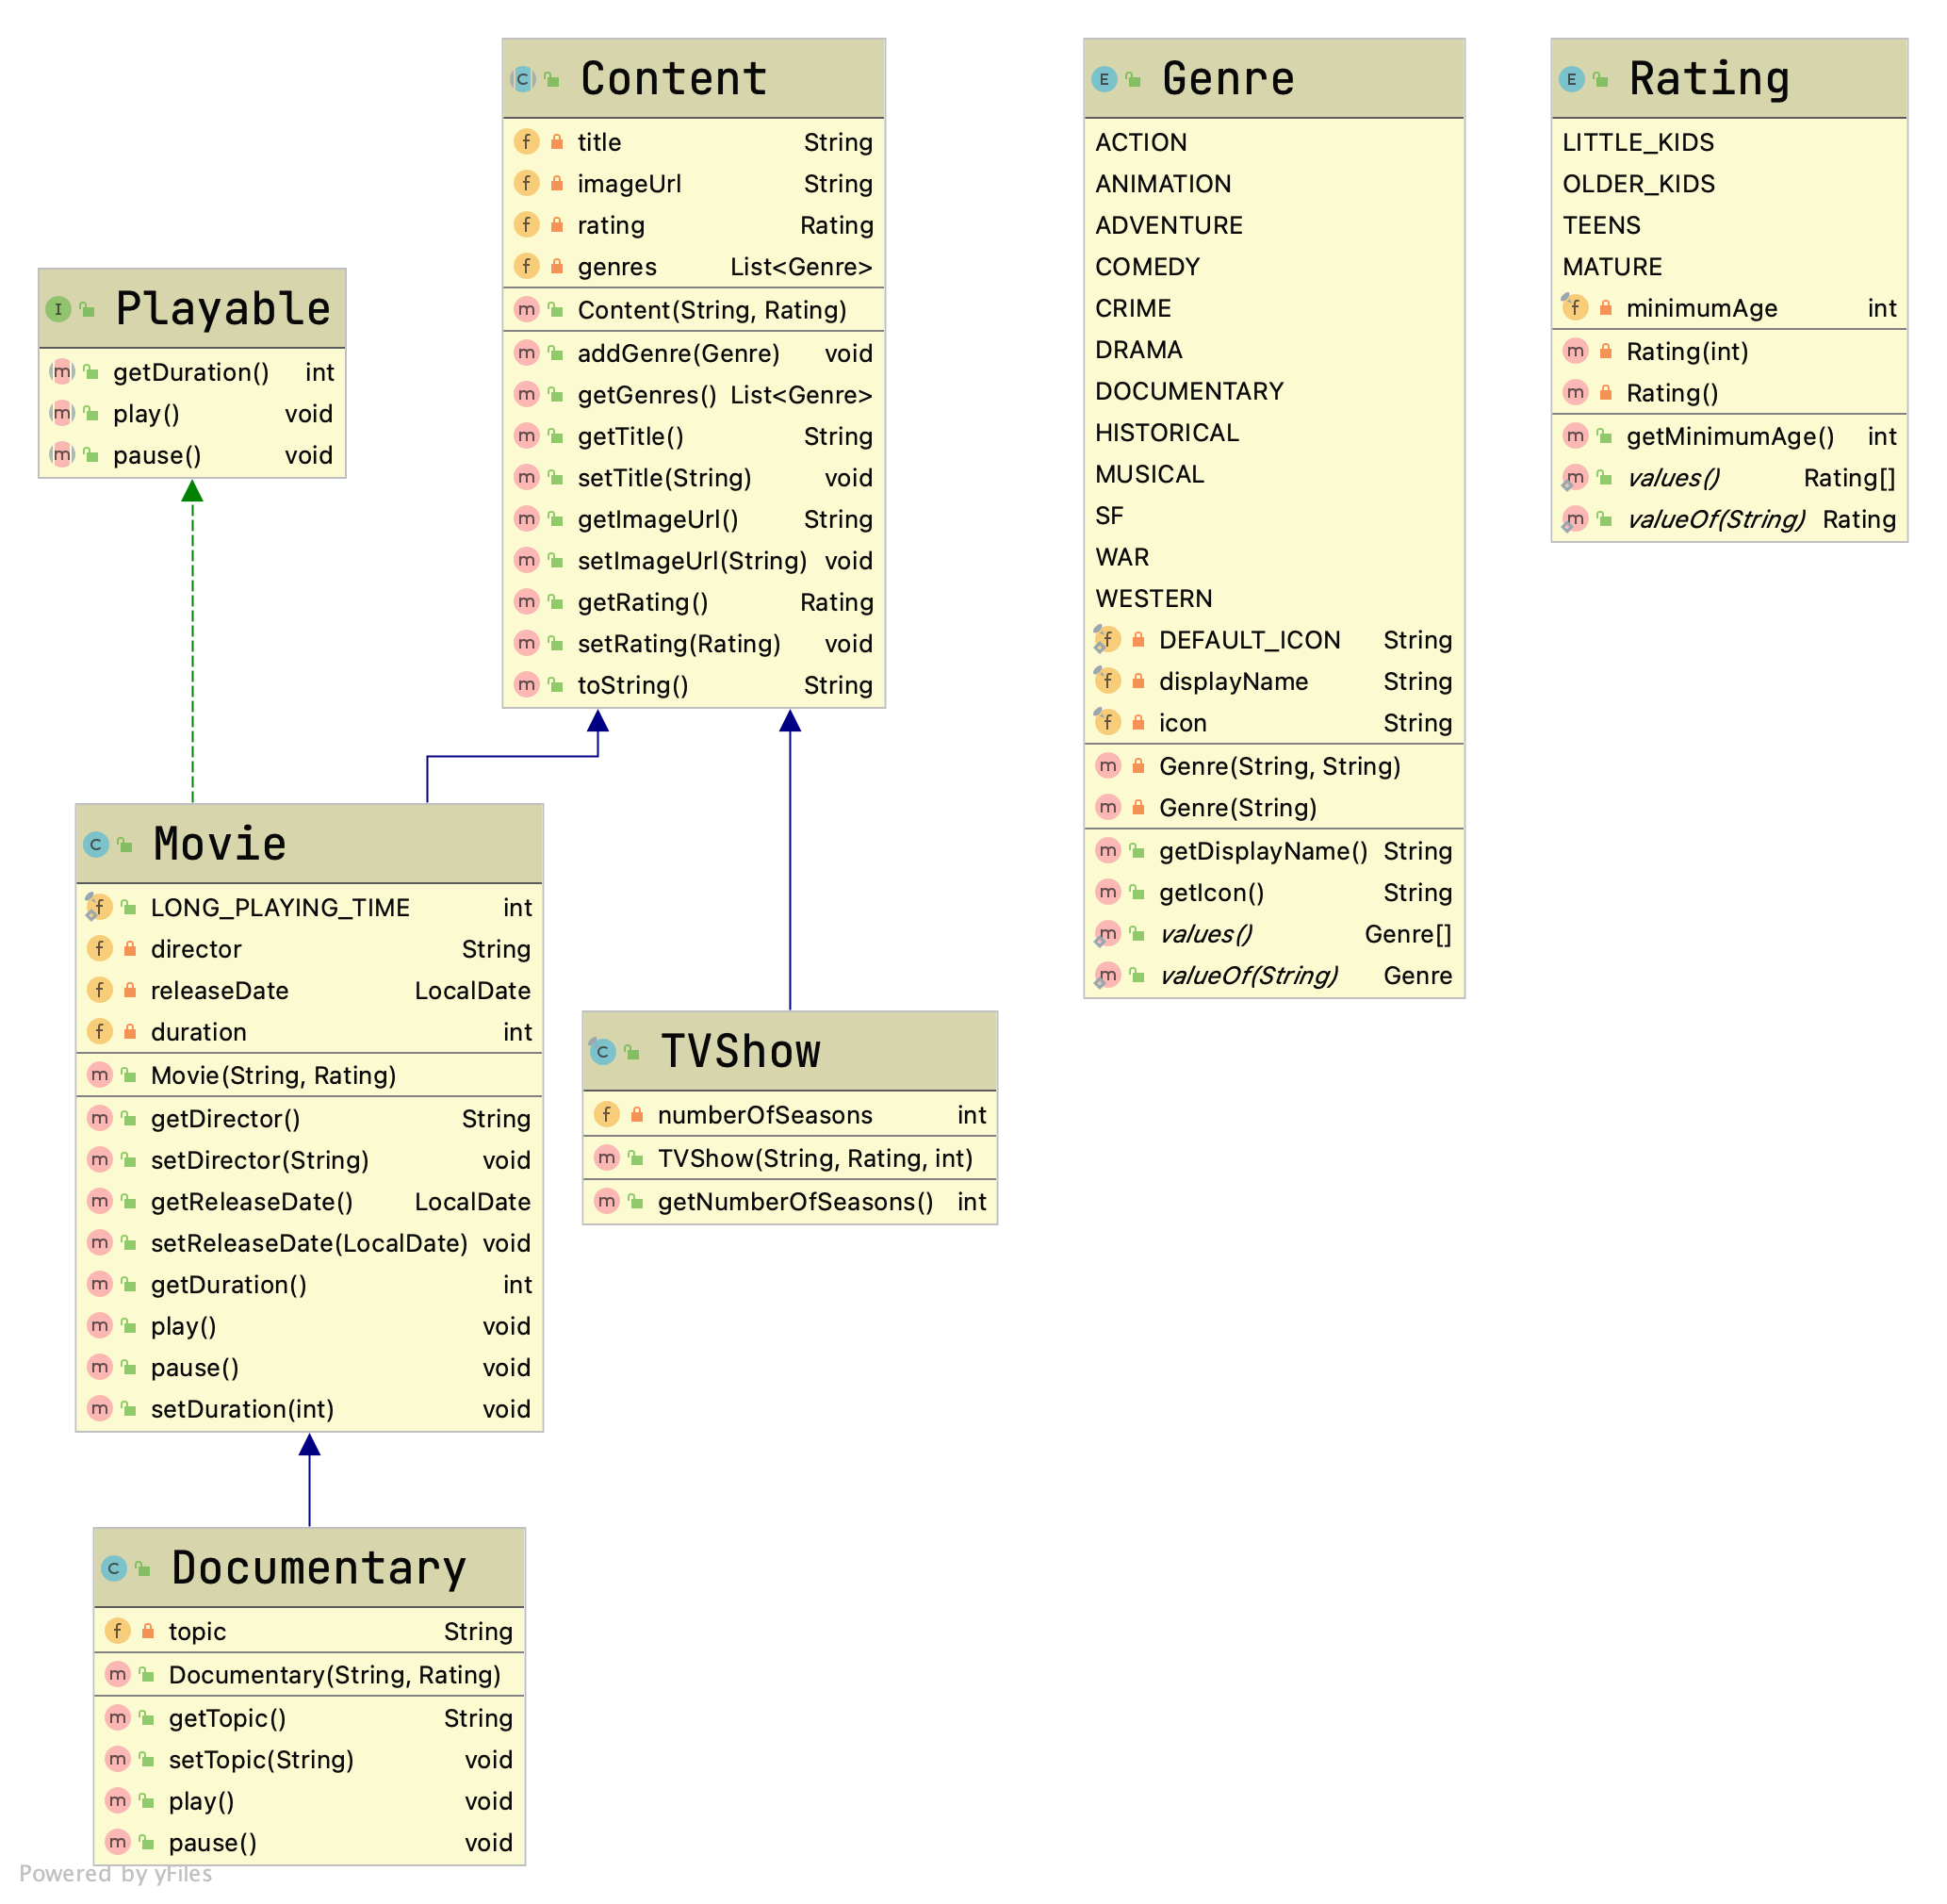
\includegraphics[width=\linewidth]{images/h1/klassendiagram_final.png}
  \caption{Klassendiagram}
  \label{fig:klassendiagram}
\end{figure}


\chapter{Unit testing}

\begin{summary}
De software die we ontwikkelen moet kwaliteitsvol zijn. Maar hoe kunnen we er nu voor zorgen dat we het aantal bugs in onze code zo laag mogelijk houden? E\'en van de strategie\"en om de kwaliteit van software te waarborgen is testen. Testen is een heel belangrijk aspect van softwareontwikkeling waar je ongetwijfeld nog heel veel over gaat leren. 

Als ontwikkelaar zorg je er altijd voor dat wanneer je de gevraagde functionalteit implementeert, je ook de nodige unit testen schrijft om de kwaliteit van je code te garanderen. Wanneer je unit testen schrijft, ga je alle methoden van je klasse testen. Een methode van een klasse is dus de ``unit'' die we gaan testen.
We gaan automatische testen schrijven. Dit betekent dat iedere keer dat de code wordt aangepast of uitgebreid de testen eenvoudig opnieuw kunnen worden uitgevoerd. Op die manier gaan de fouten die ontstaan tijdens de verdere ontwikkeling van de software snel ontdekt worden. Bedenk ook dat een fout, onduidelijkheid of bug die vroeg in het ontwikkelproces wordt aangepakt, maar een kleine impact heeft (ook financieel) ten opzicht van problemen die later pas opduiken.
\end{summary}

\section{JUnit}

In Java gaan we gebruikmaken van het framework JUnit5 om onze unit testen te schrijven.
JUnit5 is opgedeeld in 3 sub-projecten:  Jupiter, Vintage en Platform. JUnit Jupiter is het  sub-project dat wij gebruiken om onze testen te schrijven en voorziet de engine om deze testen uit te voeren.

\section{Unit test voor een constructor}

We starten direct met een voorbeeld. In het vorige hoofdstuk hadden we de klasse Documentary aangemaakt. De klasse Documentary is een subklasse van Movie. Bij het aanmaken van een Documentary-object moet wel steeds als genre Genre.DOCUMENTARY ingevuld zijn. 

\begin{lstlisting}
package be.pxl.ja.opdracht1;

public class Documentary extends Movie {

	private String topic;

	public Documentary(String title, Rating rating) {
		super(title, rating);
		addGenre(Genre.DOCUMENTARY);
	}

	public String getTopic() {
		return topic;
	}

	public void setTopic(String topic) {
		this.topic = topic;
	}
}
\end{lstlisting}

We gaan dus de constructor van de klasse Documentary testen.

Onze testklassen gaan we niet mengen met onze eigenlijke programma. Ons hoofdprogramma en de klassen zitten meestal in een source-folder (src). Onze unit testen plaatsen we in een overeenkomstig package in de test-folder. Wanneer je een folder met de naam ``test'' hebt aangemaakt, markeer deze dan ook als test-folder.

\begin{figure}[H]
  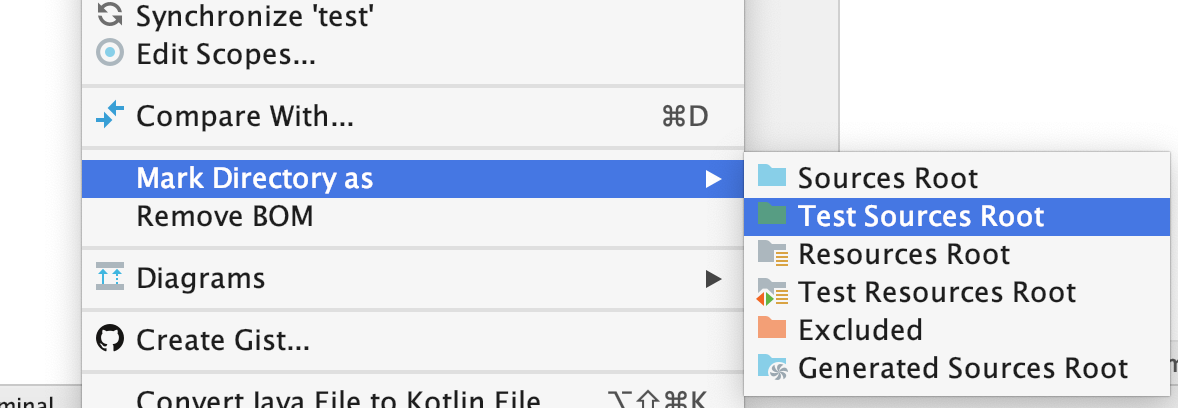
\includegraphics[width=\linewidth]{images/h1/test_directory.png}
  \caption{Markeren als test-folder}
  \label{fig:test_folder}
\end{figure}

\begin{lstlisting}
package be.pxl.ja.opdracht1;

import org.junit.jupiter.api.Test;

import static org.junit.jupiter.api.Assertions.assertEquals;

public class DocumentaryTest {

	private static final String TITLE = "Planet Earth";

	@Test
	public void documentaryConstructor() {
		// ACT
		Documentary documentary = new Documentary(TITLE, Rating.TEENS);

		// ASSERT
		assertEquals(TITLE, documentary.getTitle());
		assertEquals(Rating.TEENS, documentary.getRating());
		assertEquals(Genre.DOCUMENTARY, documentary.getGenre());
	}
}
\end{lstlisting}

\global\csname @topnum\endcsname 0

We hoeven enkel een @Test annotatie toe te voegen opdat een test herkend wordt en uitgevoerd kan worden. De eerste keer dat je de annotatie @Test toevoegt in het project zal deze nog niet gekend zijn. IntelliJ zal zelf voorstellen om JUnit te downloaden en toe te voegen aan het classpath. Zorg er wel voor dat je de juiste versie gebruikt. 

\begin{figure}[H]
  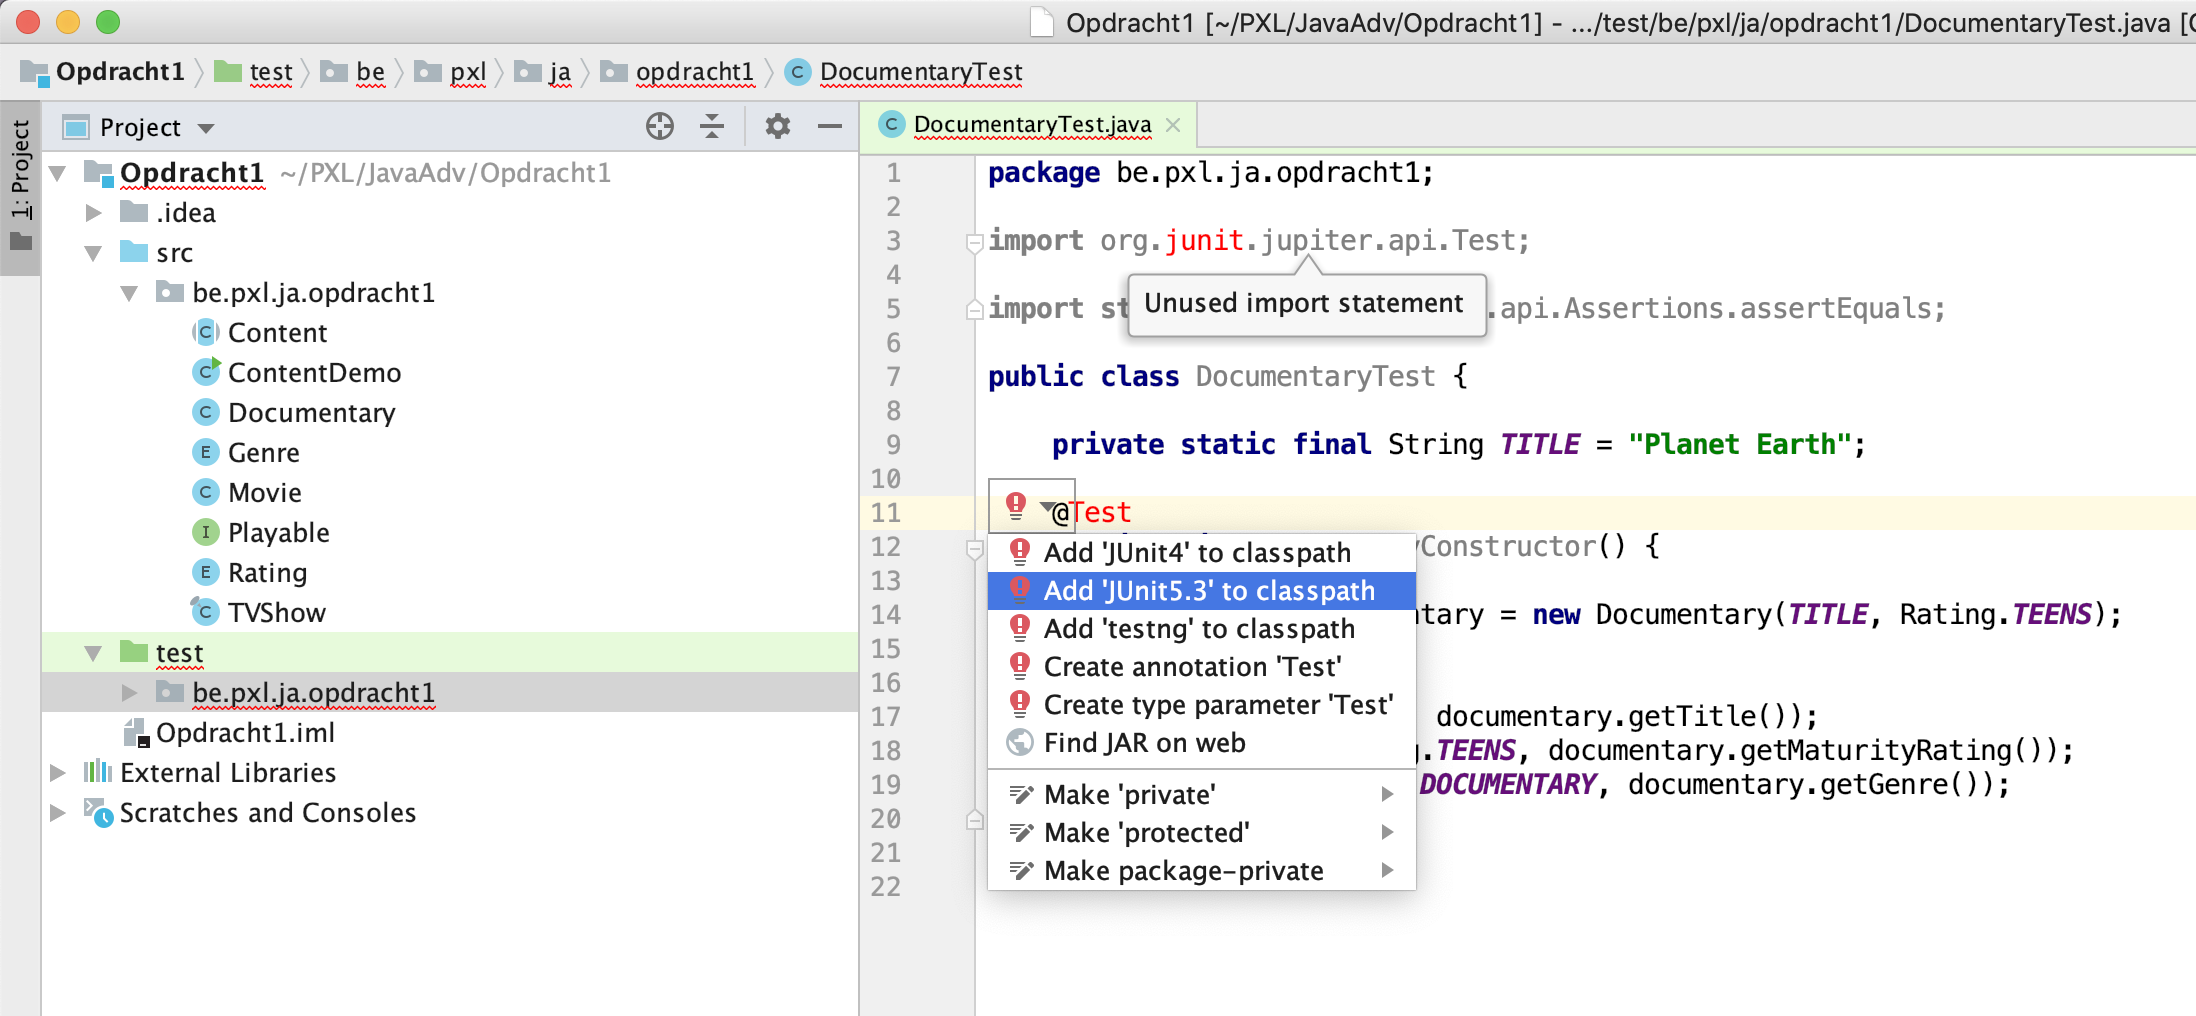
\includegraphics[width=\linewidth]{images/h1/junit_dependency.png}
  \caption{JUnit5 toevoegen aan het classpath}
  \label{fig:junit_dependency}
\end{figure}

Wanneer je nu de unit test DocumentaryTest uitvoert kunnen er 3 mogelijke scenario's plaatsvinden. Ofwel slaagt de test, ofwel faalt \'e\'en van de beweringen (asserts) ofwel loopt er iets onverwachts fout. In het eerste geval krijgt je test een groene kleurcode, in het tweede scenario een oranje en in het laatste scenario een rode.

\begin{figure}[H]
  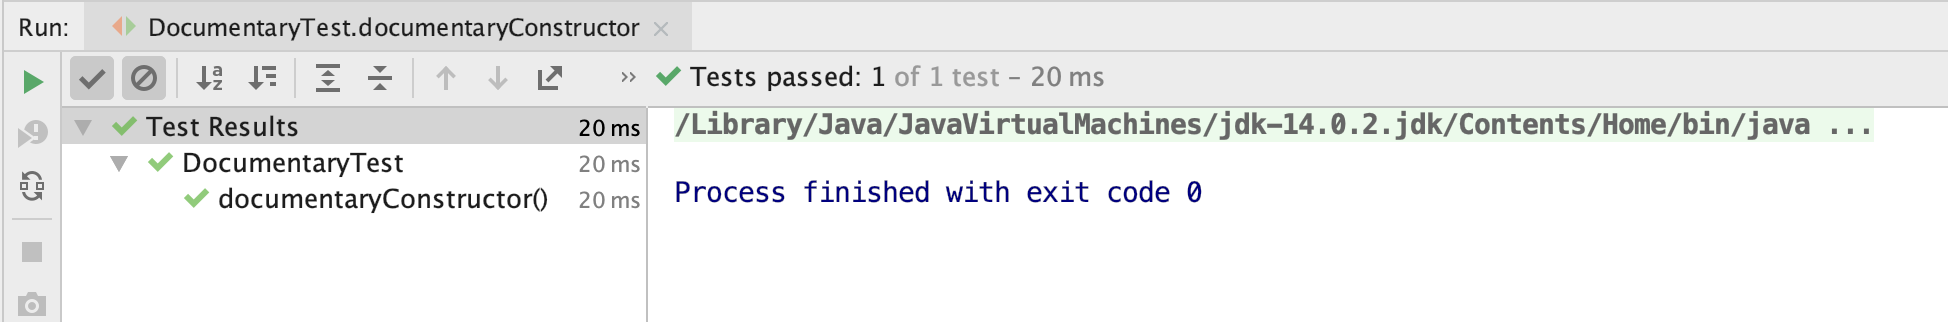
\includegraphics[width=\linewidth]{images/h1/junit_test_passed.png}
  \caption{Geslaagde JUnit5 test}
  \label{fig:test_passed}
\end{figure}

\begin{figure}[H]
  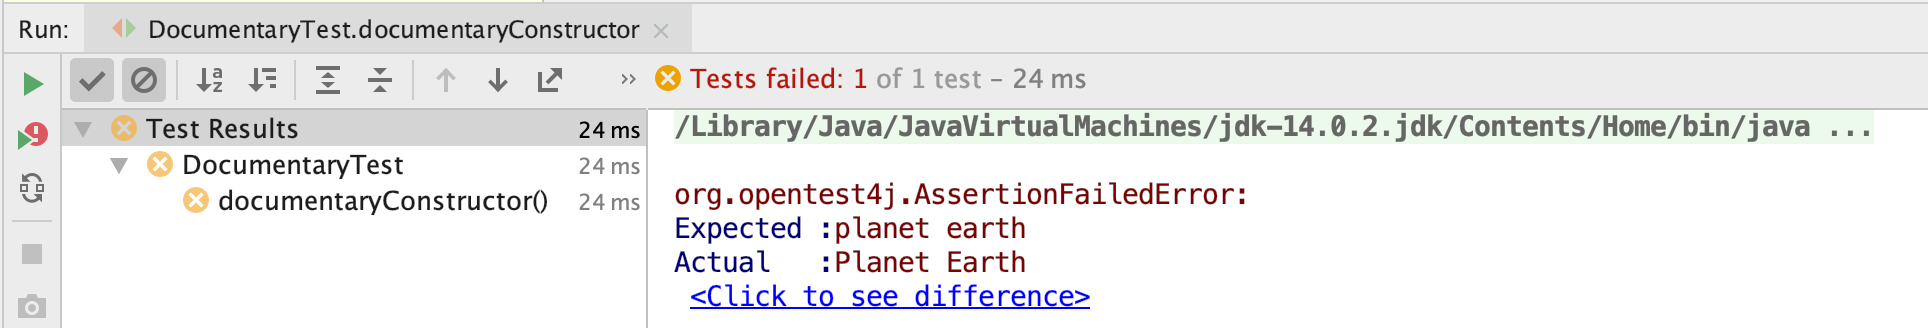
\includegraphics[width=\linewidth]{images/h1/junit_test_failed.png}
  \caption{Gefaalde JUnit5 test}
  \label{fig:test_failed}
\end{figure}

\section{Unit test voor een setter}

Onze test zal steeds opgebouwd worden volgens het 3A patroon: Arrange, Act en Assert.
In iedere test herken je steeds deze 3 bouwstenen. 

Het ``arrange''-gedeelte is waar het object dat getest moet worden en alle andere objecten - die nodig zijn om de test goed uit te voeren - worden aangemaakt. 
Het ``act''-gedeelte is waar we de methode die we willen testen aanroepen. Als de methode een returnwaarde heeft ken je dit toe aan een variabele.

Het ``assert''-gedeelte geeft je de mogelijkheid om beweringen over het resultaat te verifi\"eren.

Hier is nog eens de klasse Movie.

\begin{lstlisting}
import java.time.LocalDate;

public class Movie extends Content implements Playable {
	private String director;
	private LocalDate releaseDate;
	private int duration;

	public Movie(String title, Rating rating) {
		super(title, rating);
	}

	public String getDirector() {
		return director;
	}

	public void setDirector(String director) {
		this.director = director;
	}

	public LocalDate getReleaseDate() {
		return releaseDate;
	}

	public void setReleaseDate(LocalDate releaseDate) {
		this.releaseDate = releaseDate;
	}

	public int getDuration() {
		return duration;
	}

	@Override
	public void play() {
		System.out.println("Playing " + this);
	}

	@Override
	public void pause() {
		System.out.println("Pausing " + this);
	}

	public boolean isLongPlayingTime() {
		return duration > LONG_PLAYING_TIME;
	}

	public String getPlayingTime() {
		// TODO: implement this method correctly		
		return "2 u 30 min";
	}

	@Override
	public String toString() {
		StringBuilder builder = new StringBuilder(super.toString());
		if (releaseDate != null) {
			builder.append(" (").append(releaseDate.getYear()).append(")");
		}
		return builder.toString();
	}
}
\end{lstlisting}

\global\csname @topnum\endcsname 0

Bekijk de methode void setDuration(int duration) eens. We willen nooit een negatief getal als waarde voor de eigenschap duration. Daarom zullen we de absolute waarde nemen van de parameter duration. Om deze setter te testen gaan we 2 testen voorzien. Een eerste test waar we een positieve waarde meegeven als argument en een tweede test waarbij we een negatieve waarde meegeven.

\begin{lstlisting}
import org.junit.jupiter.api.Test;

import static org.junit.jupiter.api.Assertions.assertEquals;

public class MovieSetDurationTest {

	@Test
	public void negativeDurationBecomesPositive() {
		// ARRANGE
		Movie movie = new Movie("Titanic", Rating.OLDER_KIDS);

		// ACT
		movie.setDuration(-125);

		// ASSERT
		assertEquals(125, movie.getDuration());
	}

	@Test
	public void positiveDurationStaysUnchanged() {
		// ARRANGE
		Movie movie = new Movie("Titanic", Rating.OLDER_KIDS);

		// ACT
		movie.setDuration(125);

		// ASSERT
		assertEquals(125, movie.getDuration());
	}
}
\end{lstlisting}

\clearpage

\section{Unit test voor een getter}

In de klasse Movie vind je ook de methode isLongPlayingTime() terug. Deze methode heeft een boolean als resultaat-type en geeft true indien de film langer dan 2 u 15 min duurt.

Hier is alvast 1 mogelijke unit test.

\begin{lstlisting}
import static org.junit.jupiter.api.Assertions.assertFalse;

public class MovieIsLongPlayingTimeTest {
	
	@Test
	public void movieWithDurationShorterThanLongPlayingTimeReturnsFalse() {
		
		Movie movie = new Movie("Titanic", Rating.TEENS);
		
		movie.setDuration(Movie.LONG_PLAYING_TIME - 1);
		
		assertFalse(movie.isLongPlayingTime());
	}
}
\end{lstlisting}

Bij de overige testen zullen in het Arrange gedeelte opnieuw een Movie-object moeten aanmaken. Omdat dit voor iedere test herzelfde is, hoeven we deze code niet te dupliceren. 
Met de annotatie @BeforeEach kunnen we een methode aanduiden die wordt uitgevoerd voor elke test.

Daarnaast merk je ook dat de klasse org.junit.jupiter.api.Assertions bijkomende static methoden heeft om de resultaten van de test te verifi\"eren. \textbf{assertFalse} en \textbf{assertTrue} zullen  slagen als de getestte waarde repectievelijk false of true is.

\begin{lstlisting}
import org.junit.jupiter.api.BeforeEach;
import org.junit.jupiter.api.Test;

import static org.junit.jupiter.api.Assertions.assertFalse;
import static org.junit.jupiter.api.Assertions.assertTrue;

public class MovieIsLongPlayingTimeTest {

	private Movie movie;

	@BeforeEach
	public void init() {
		movie = new Movie("Titanic", Rating.TEENS);
	}

	@Test
	public void movieWithDurationShorterThanLongPlayingTimeReturnsFalse() {

		movie.setDuration(Movie.LONG_PLAYING_TIME - 1);

		assertFalse(movie.isLongPlayingTime());
	}

	@Test
	public void movieWithDurationExactlyLongPlayingTimeReturnsFalse() {

		movie.setDuration(Movie.LONG_PLAYING_TIME);

		assertFalse(movie.isLongPlayingTime());
	}

	@Test
	public void movieWithDurationLongerThanLongPlayingTimeReturnsTrue() {

		movie.setDuration(Movie.LONG_PLAYING_TIME + 1);

		assertTrue(movie.isLongPlayingTime());
	}
}
\end{lstlisting}

We maken ook in de testen handig gebruik van de constante LONG\_PLAYING\_TIME. Door onze testen op deze manier te schrijven hoeven we de testen niet aan te passen als de waarde van LONG\_PLAYING\_TIME wordt aangepast. 

Hier is een overzicht van enkele handige static methoden uit de klasse org.junit.jupiter.api.Assertions. 

\begin{table}[h!]
\centering
\begin{tabularx}{\textwidth}{| l | X |}
 \hline
 Methode & Betekenis\\ 
 \hline\hline
assertEquals() & Evalueert de gelijkheid van 2 waarden. De test slaagt als beide
waarden gelijk (equal) zijn.\\
\hline
assertFalse() & Evaluatie van een booleaanse uitdrukking. De test slaagt indien
de uitdrukking false is.\\
\hline
assertTrue() & Evaluatie van een booleaanse uitdrukking. De test slaagt indien
de uitdrukking true is.\\
\hline
assertNotNull( ) & Vergelijkt een object referentie met null. De test slaagt indien de
object referentie niet null is.\\
\hline
assertSame( ) & Vergelijkt het geheugenadres van twee object referenties
(gebruik maken van == operator). De test slaagt indien beide
object referenties naar hetzelfde object verwijzen.\\
\hline
fail() & Zorgt ervoor dat de test zal falen.\\
 \hline
\end{tabularx}
\caption{Static methoden uit de klasse org.junit.jupiter.api.Assertions}
\label{table:assertions}
\end{table}

\begin{oefening}
Schrijf 2 unit testen voor de toString() methode van de klasse Movie. We verwachten dat deze methode de titel en het jaartal van de film teruggeeft (bijv. Titanic (1997)). Indien er geen releasedatum gekend is, wordt het jaartal achterwege gelaten.
\end{oefening}

\begin{oefening}
Schrijf unit testen voor de methode addGenre in de klasse Content. Let er ook op dat een  genre enkel wordt toegevoegd indien het niet eerder al werd toegevoegd. 
\end{oefening}

\begin{oefening}
Je ziet dat in bovenstaande klasse Movie de methode getPlayingTime() nog niet correct ge\"implementeerd is. Hier zijn alvast de unit testen. 

\begin{lstlisting}
import org.junit.jupiter.api.BeforeEach;
import org.junit.jupiter.api.Test;

import static org.junit.jupiter.api.Assertions.assertEquals;

public class MovieGetPlayingTimeTest {

	private Movie movie;

	@BeforeEach
	public void init() {
		movie = new Movie("Titanic", Rating.OLDER_KIDS);
	}

	@Test
	public void returnsQuestionmarkWhenDurationZero() {

		movie.setDuration(0);

		assertEquals("?", movie.getPlayingTime());
	}

	@Test
	public void returnsMinutesWhenDurationLessThan60() {

		movie.setDuration(59);

		assertEquals("59 min", movie.getPlayingTime());
	}

	@Test
	public void returnsHoursWhenDurationMultipleOf60() {

		movie.setDuration(120);

		assertEquals("2 h", movie.getPlayingTime());
	}

	@Test
	public void returnsHoursAndMinutesWhenDurationNotMultipleOf60() {

		movie.setDuration(135);

		assertEquals("2 h 15 min", movie.getPlayingTime());
	}
}
\end{lstlisting}

Bestudeer deze unit testen en implementeer vervolgens de methode. Test je implementatie uit! Wanneer alle testen slagen, bekijk dan je je code nog eens kritisch. Kan je nog verbeteringen aanbrengen in de code?
\end{oefening}

Je ziet dat je geen schrik moet hebben om achteraf je code te verbeteren. Omdat je beschikt over unit testen kan je rustig aan je code gaan sleutelen. Het proces om code te verbeteren en hierdoor de leesbaarheid en onderhoudbaarheid van de code te verhogen noemen we \textbf{refactoren}. 

\begin{remark}
  Meer weten over unit testing, kijk op pluralsight: \url{https://app.pluralsight.com/library/courses/junit-5-unit-testing-getting-started}
\end{remark}

\begin{oefening}
We gaan bij de domeinklassen van de streaming service nog enkele klassen en enums toevoegen. Deze klassen gaan we hergebruiken tijdens latere oefeningen. 

Je implementeert volgende enums en klassen in je oplossingen van opgave 1:
\begin{itemize}
\item CreditCardType
\item PaymentInfo
\item StreamingPlan
\item Profile
\item Account
\end{itemize}

\textbf{Enum CreditCardType}

CreditCardType is een eenvoudige enum-klasse met de waarden VISA en MASTERCARD.

\textbf{Klasse PaymentInfo}

Wanneer een gebruiker een account aanmaakt voor onze streaming service moet hij zijn betaalgegevens opgegeven. Deze gegevens houden we bij in een PaymentInfo-object.
Deze klasse bevat de volgende eigenschappen:

\begin{itemize}
\item cardNumber (String)
\item type (CreditCardType)
\item firstName (String)
\item lastName (String)
\item expirationDate (LocalDate)
\item securityCode (int)
\end{itemize}

Je hoeft enkel getters en setters te voorzien. Het valideren van cardNumber, securityCode en expirationDate houden we voor het volgende hoofdstuk wanneer we het hebben over foutafhandeling.

\textbf{Enum StreamingPlan}

Er zijn 3 producten waaruit gebruikers kunnen kiezen. Ieder product heeft een maximum aantal profielen per account en een prijs. 

Gebruikers met product BASIC kunnen maar 1 profiel aanmaken en betalen €7,99.
Gebruikers die kiezen voor STANDAARD kunnen 2 profielen aanmaken en betalen €11,99.
Tenslotte kunnen gebruikers met een PREMIUM account 4 profielen aanmaken. Zij betalen €15,99.

Maak een enum met de naam StreamingPlan met deze producten. Gebruik numberOfProfiles en price als eigenschappen voor deze enum-klasse. 

\textbf{Klasse Profile}

Afhankelijk van de StreamingPlan kunnen er dus profielen toegevoegd worden aan een account. Daarom implementeren we de klasse Profile. Voor iedere Profile-object willen we een naam (name) en een geboortedatum (dateOfBirth) weten. Deze laatste hebben we nodig om te beslissen of Content beschikbaar is of niet. 

Hiervoor voorzie je een methode \textit{boolean allowedToWatch(Content content)} in de klasse Profile. De methode geeft true als de content geschikt is voor het profiel (afhankelijk van de rating van de content en de geboortedatum van het profiel). 
De methode geeft false als de content niet geschikt is voor het profiel.
Zolang de geboortedatum niet is ingevuld is alle content niet geschikt voor het profiel.
Voeg de nodige unit testen toe om deze methode grondig te testen!

\textbf{Klasse Account}

En tenslotte voeg je de klasse Account toe. Een account heeft volgende eigenschappen:
\begin{itemize}
\item email
\item password
\item streamingPlan
\item \'e\'en of meerder profielen
\item paymentInfo
\end{itemize}

In de constructor van een Account wordt er direct 1 profiel aangemaakt met de naam "profile1" en geboortedatum 1/1/2000. Schrijf unit testen voor de constructor.

De methode getFirstProfile() geeft het eerste (en voorlopig ook enige) Profile-object terug als resultaat. 

De functionaliteit om profielen toe te voegen wordt in een volgend hoofdstuk toegevoegd.

\textbf{Optioneel: Sterkte van het paswoord}

Wanneer de gebruiker een account aanmaakt kiest hij een paswoord. We geven hem graag een indicatie of zijn gekozen paswoord voldoende sterk is.
Maak een hulpklasse \textbf{PasswordUtil}  met een static methode \textit{int calculateStrength(String password)}. 

Hier zijn de regels voor de berekening van de sterkte van een paswoord:
\begin{itemize}
\item Een paswoord met minder dan 6 karakters is zwak en geeft altijd een score van 0.
\item Een paswoord met een lengte tussen 6 en 10 geeft een score van 1.
\item Een paswoord met meer dan 10 karaketer geeft een score van 2.
\end{itemize}
Voor paswoorden met een lengte vanaf 6 karakters gelden de volgende bijkomende regels:
\begin{itemize}
\item Indien het paswoord minstens 1 cijfer bevat, wordt de score met 2 verhoogd.
\item Indien het paswoord minstens 1 kleine letter bevat, wordt de score met 2 verhoogd.
\item Indien het paswoord minstens 1 hoofdletter bevat, wordt de score met 2 verhoogd.
\item Indien het paswoord minstens 1 special karakter bevat, wordt de score met 2 verhoogd. Er is reeds een constante aanwezig in de klasse PasswordUtil die de speciale karakters bevat.
\end{itemize}
Implementeer deze regels en schrijf de nodige unit testen.
\end{oefening}

\begin{figure}[H]
  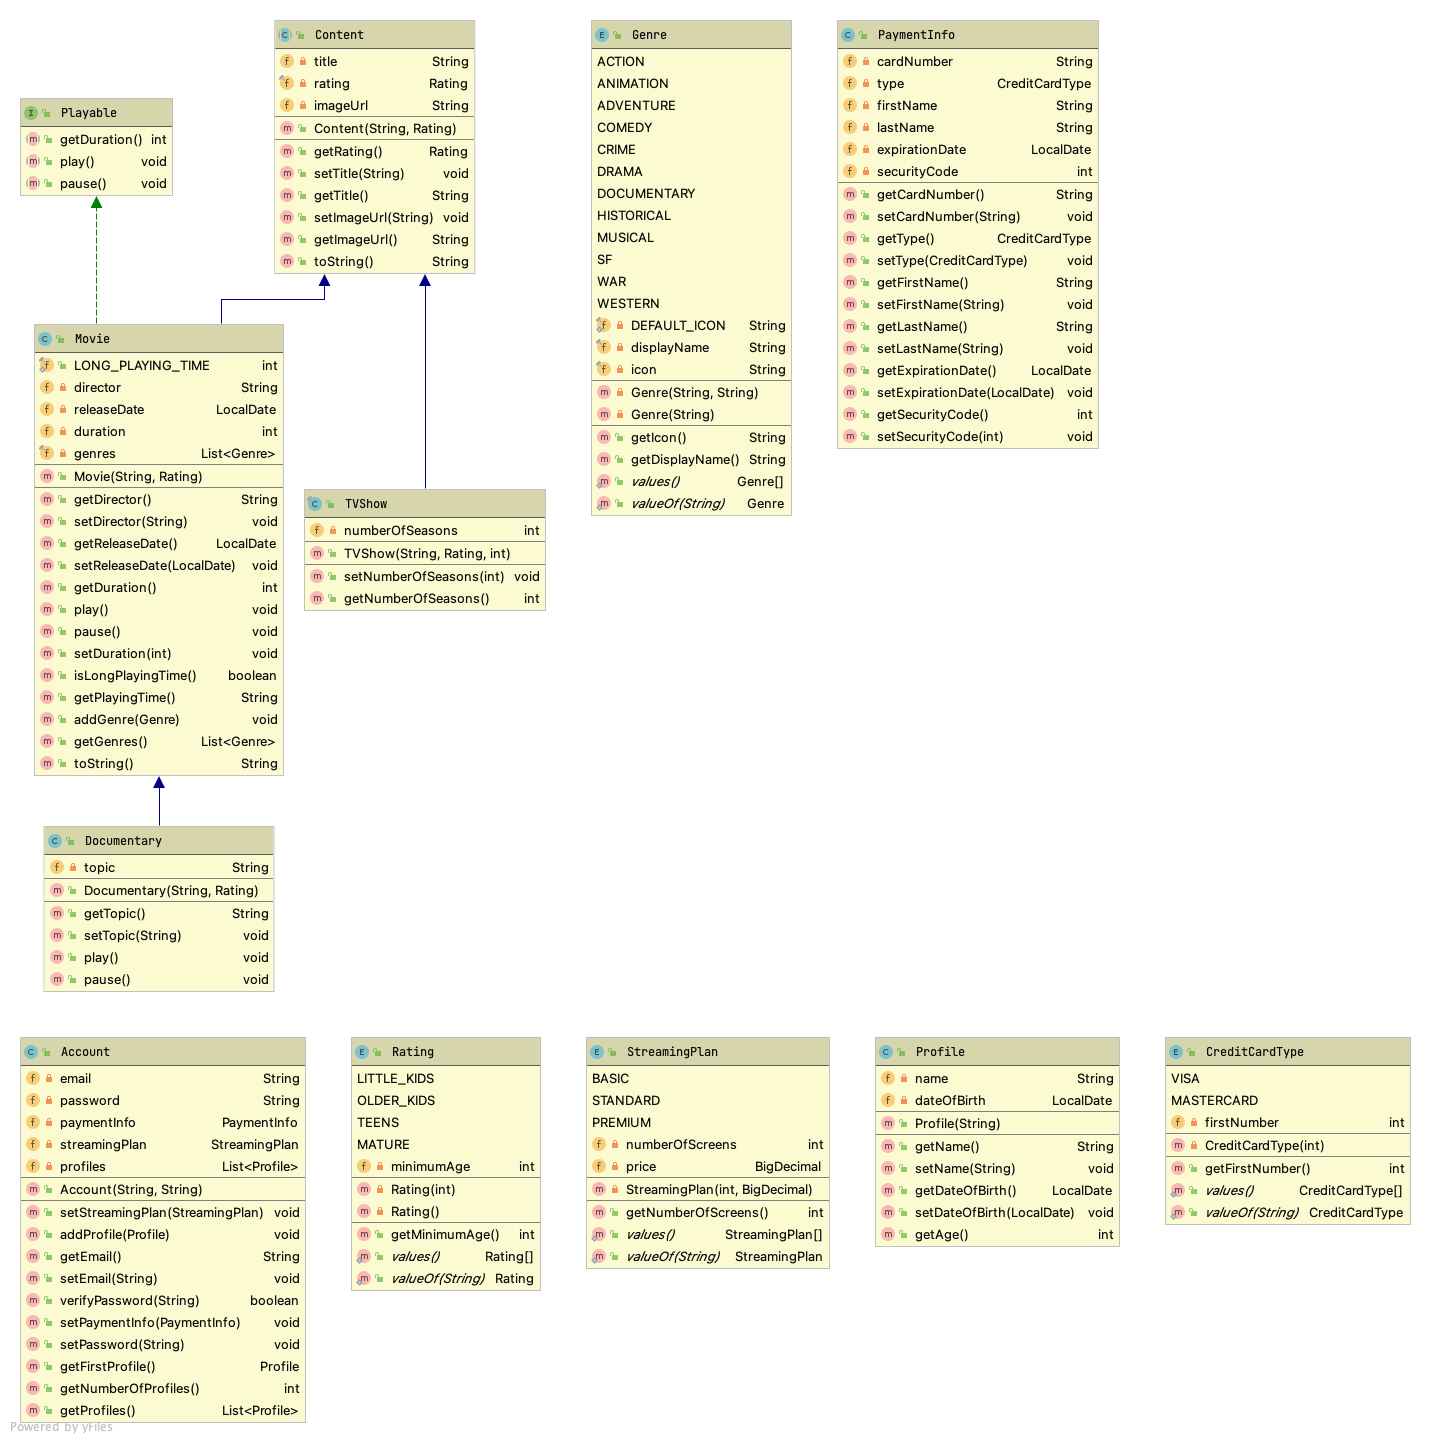
\includegraphics[width=\linewidth]{images/klassendiagram/diagram_H2.png}
  \caption{Klassendiagram}
  \label{fig:klassendiagram}
\end{figure}

\chapter{Foutafhandeling}

\begin{summary}
Tijdens het uitvoeren van een programma kan en zal er vanalles foutgaan. De gebruiker van het programma geeft de datum in in een foutief formaat, een printer is offline, er is onvoldoende schrijfruimte vrij om een bestand weg te schrijven, het programma kreeg onvoldoende geheugen toegewezen,... Fouten die zich voordoen tijdens het uitvoeren van een programma, at runtime dus, verdelen we onder in errors en exceptions. Errors zijn de fouten die meestal veroorzaakt worden door het onderliggende besturingssysteem. Tijdens het verloop van het programma kunnen deze errors niet meer opgelost worden en het programma zal daarom be\"eindigd worden. Dit is niet het geval voor exceptions. Je kan je code op een defensieve manier schrijven en rekening houden met de mogelijke exceptions die kunnen optreden. ``Exception handling'' is het proces om deze exceptions op een correcte en liefst gebruiksvriendelijke manier af te handelen. Indien een fout niet correct wordt afgehandeld, zal het programma alsnog voortijdig afgebroken worden, maar met de juiste foutafhandeling kan de uitvoer van het programma gewoon verdergezet worden. 
 \end{summary}
 
\section{Compile-time vs runtime errors}

Een programmeur schrijft Java code in zijn editor of favoriete IDE. Vervolgens wordt de Java code gecompileerd tot bytecode. Deze bytecode wordt door de JVM (Java Virtual Machine) ge\"interpreteerd tot machinecode instructies die worden uitgevoerd door het computersysteem.

Wanneer dus een Java programma wordt opgestart, kunnen er 2 categorie\"en van problemen voorkomen. Het kan zijn dat het Java programma niet gecompileerd kan worden. In dat geval spreken we van een compile-time error. Indien het programma succesvol gecompileerd wordt, kan er zich tijdens het uitvoeren van de code een probleem voordoen, in dat geval spreken we van runtime errors of exceptions. 

\begin{figure}[H]
  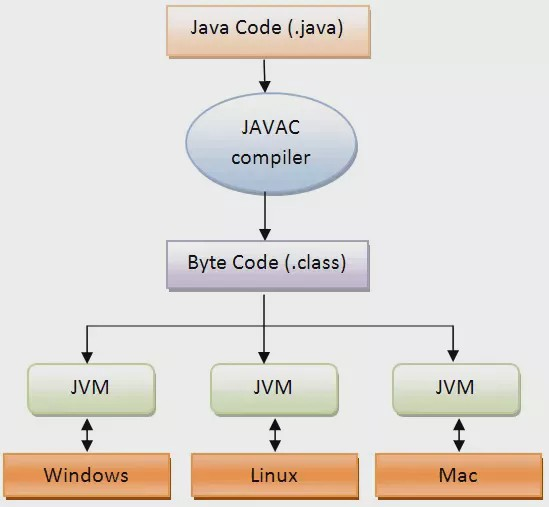
\includegraphics[width=\linewidth]{images/h1/java_compiler.jpeg}
  \caption{Compiler, interpreter en Java Virtual Machine.}
  \label{fig:compiler}
\end{figure}


\begin{figure}[H]
  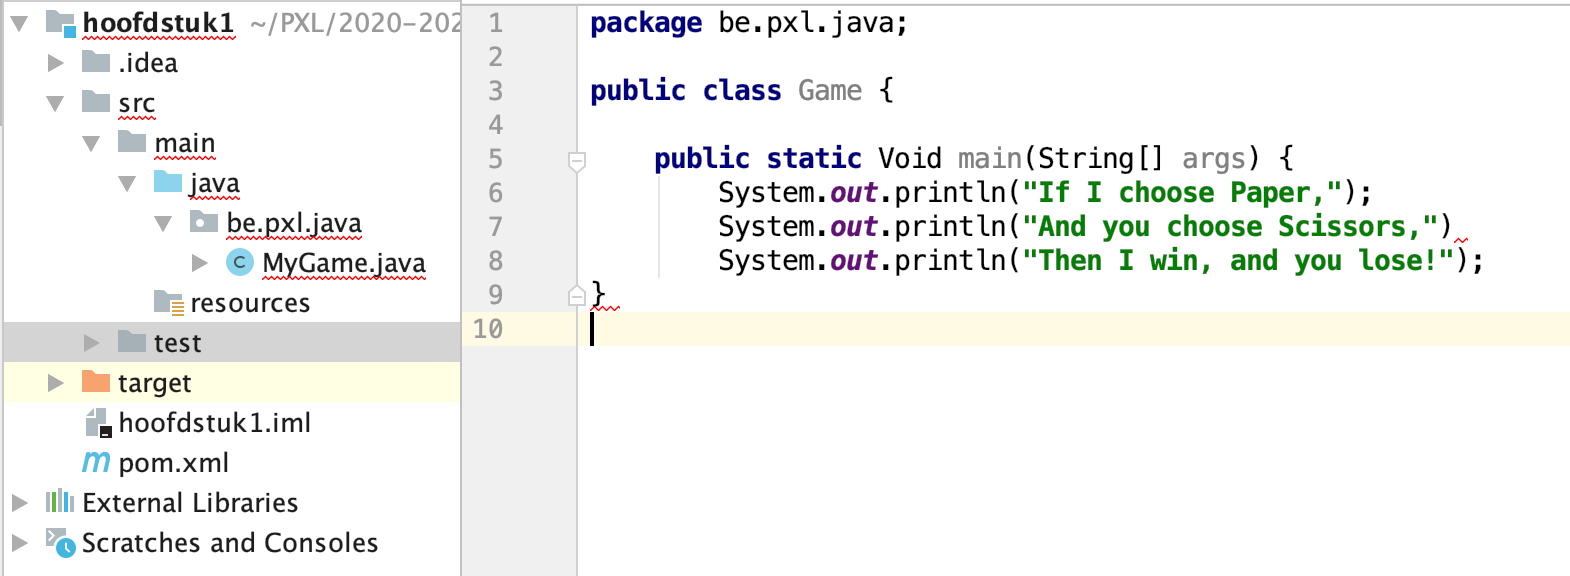
\includegraphics[width=\linewidth]{images/h1/compiletime_errors.png}
  \caption{Compile-time errors}
  \label{fig:compiletime_errors}
\end{figure}

\begin{oefening}
Welke compile-time errors kan je ontdekken in het volgende codefragment in figuur \ref{fig:compiletime_errors}?
\end{oefening}

Omdat Java een object-ge\"orienteerde programmeertaal is, wordt er ook een object gebruikt om aan te geven dat er iets fout ging bij uitvoeren van het Java programma. Zodra er zich een probleem voordoet tijdens het uitvoeren van een programma-instructie, wordt er een exception-object aangemaakt en ``opgeworpen''. Hierdoor stopt de normale uitvoer van het programma. Er wordt nog geprobeerd om het exception-object op een keurige manier af te handelen (indien die code aanwezig is), maar als dat niet lukt zal het programma be\"eindigd worden. Het exception-object bevat nuttige informatie voor de ontwikkelaar zoals de methode en lijn-nummer waar de exception werd aangemaakt en het type van de exception. 

\section{First catch}

\begin{lstlisting}
public class DivisionByZero {

	public static void main(String[] args) {
		int a = (1 + 1) % 2;
		int b = 5;
		int c = b / a;
		System.out.println("Het resultaat is " + c);
	}
}
\end{lstlisting}

Als je het bovenstaande programma uitvoert zal het volgende in de console verschijnen:

\begin{verbatim}
Exception in thread "main" java.lang.ArithmeticException: / by zero
	at be.pxl.ja.DivisionByZero.main(DivisionByZero.java:6)<5 internal calls>
\end{verbatim}
  
De variabele \textit{a} bevat inderdaad de waarde 0 en hierdoor hebben we dus te maken met een deling door 0. Zodra de deling wordt uitgevoerd loopt het dus fout en gooit de java runtime een ArithmeticException op. Omdat de ArithmeticException nergens wordt afgehandeld eindigt het programma. Je zal enkel nog een stacktrace zien verschijnen in de console. Een stacktrace is de naam en foutboodschap van de exception gevolgd door de weg die de exception heeft afgelegd (doorheen de methoden van je klassen) vanaf het moment dat ze werd opgegooid. We zien dus dat de exception is veroorzaakt op regel 6 in de klasse DivisionByZero.

\begin{lstlisting}
public class DivisionByZero {

	public static void main(String[] args) {
		int a = (1 + 1) % 2;
		int b = 5;
		try {
			int c = b / a;
			System.out.println("Het resultaat is " + c);
		} catch (ArithmeticException e) {
			System.out.println("You should not divide a number by zero.");
		}
		System.out.println("First catch completed!");
	}
}
\end{lstlisting}

\begin{verbatim}
You should not divide a number by zero.
First catch completed!
\end{verbatim}

We hebben de instructie met de deling nu in een try-blok geplaatst. Omdat de variabele c in het try-blok wordt aangemaakt, kan deze variabele ook enkel binnen het try-blok gebruikt worden. Indien een exception optreedt binnen een try-blok zal de programma-uitvoer de resterende code binnen het try-blok overslaan en verdergaan bij het eerste catch-blok dat direct volgt achter het try-blok. Je bent als programmeur verplicht om een try-blok steeds te laten volgen door \'e\'en of meerdere catch-blokken.
In het catch-blok wordt dan de code uitgevoerd om het probleem op te lossen of tenminste een duidelijke boodschap voor de gebruiker van het programma te voorzien.
Als alle instructies uit het catch-blok zijn uitgevoerd zal het programma zijn normale uitvoer verderzetten.


\section{Java exception hi\"erarchie}
  
\begin{figure}[H]
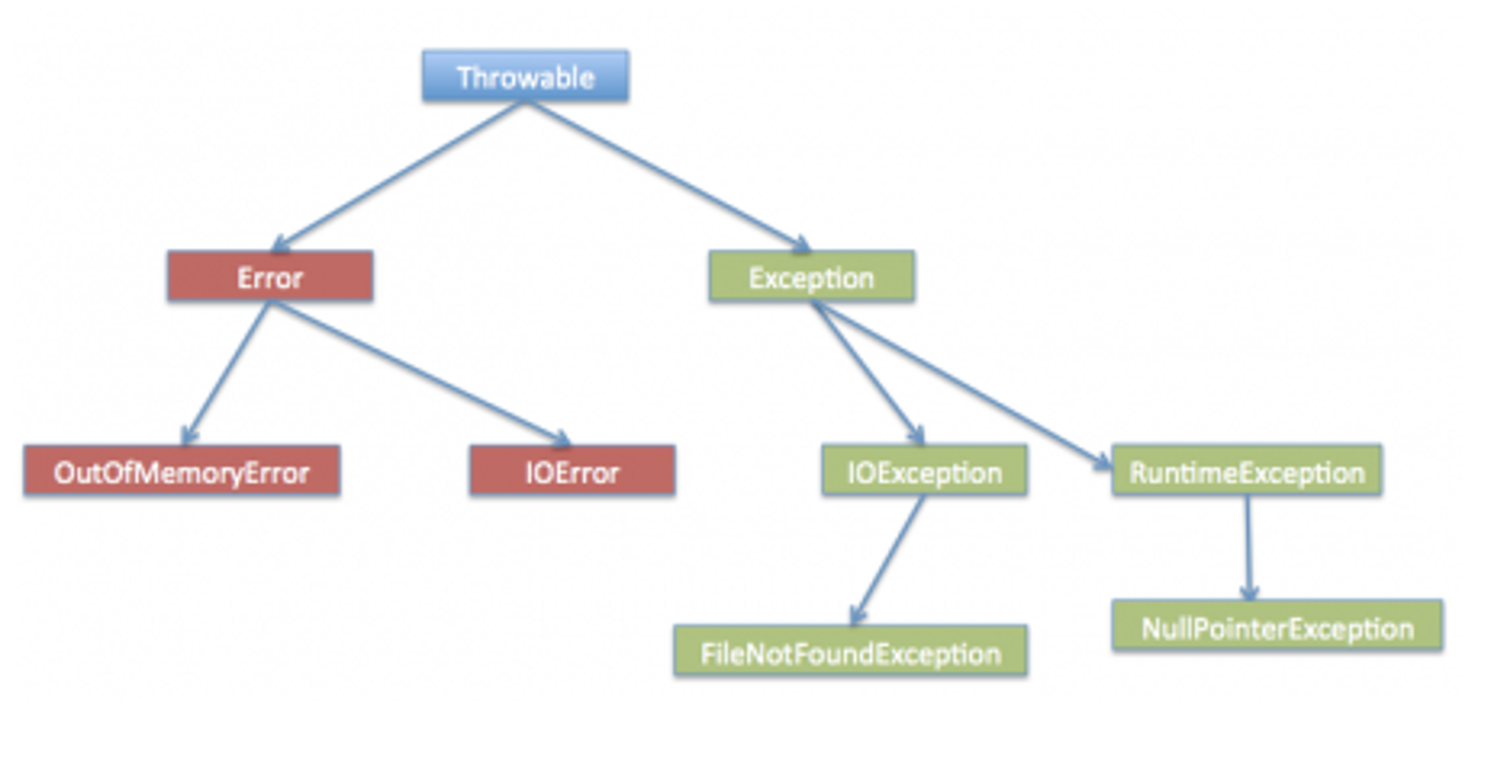
\includegraphics[width=\linewidth]{images/h1/exception-hierarchy.png}
\caption{Exception hi\"erarchie}
\label{fig:exceptiono_hierarchy}
\end{figure}
  
Zoals reeds vermeld wordt er een exception-object aangemaakt zodra zich een probleem voordoet in de code. 
Er is in Java een hi\"erarchie gebouwd van exception-klassen om verschillende soorten fouten in een programma te categorizeren. Throwable is de superklasse van alle exceptions en errors in Java. Er zijn dus 2 afgeleide klassen van Throwable: Error and Exception. Exceptions zijn nog verder onderverdeeld in \textbf{checked exceptions} en \textbf{runtime exceptions}.

\subsection{Errors}

Errors zijn problemen die zich voordoen tijdens het uitvoeren van het programma en die meestal niet gerelateerd zijn aan het programma zelf. Daarom is het onmogelijk om erop te anticiperen en te herstellen van deze fouten. Dit kan gaan van hardware falen, over JVM crashes en out of memory errors. We hebben een aparte hi\"erarchie van errors en we zullen nooit code toevoegen in ons programma om deze fouten af te handelen. We tonen hier enkel voorbeelden van errors.


\subsubsection{StackOverflowError}
Je hebt ongetwijfeld al eens per ongeluk een programma geschreven met een oneindige lus. 

\begin{lstlisting}
public class DemoStackOverflow {

	private static void printNumber(int x) {
		System.out.println(x);
		printNumber(x + 2);
	}

	public static void main(String[] args) {
		printNumber(15);
	}
}
\end{lstlisting}

\begin{verbatim}
15
17
19
...
36597
36599
Exception in thread "main" java.lang.StackOverflowError
	...
	at be.pxl.ja.DemoStackOverflow.printNumber(DemoStackOverflow.java:5)
	at be.pxl.ja.DemoStackOverflow.printNumber(DemoStackOverflow.java:5) 
	at be.pxl.ja.DemoStackOverflow.printNumber(DemoStackOverflow.java:5) 
	at be.pxl.ja.DemoStackOverflow.printNumber(DemoStackOverflow.java:5) 
	...
\end{verbatim}

De call stack is de manier waarop tijdens de uitvoer van een programma o.a. wordt bijgehouden welke functies worden aangeroepen. Wanneer je programma-uitvoer in een oneindige lus terechtkomt, stapelen de gegevens in de call stack zich razendsnel op en loopt de call stack vol. Het programma zal uiteindelijk eindigen met een StackOverflowError.

\begin{figure}[H]
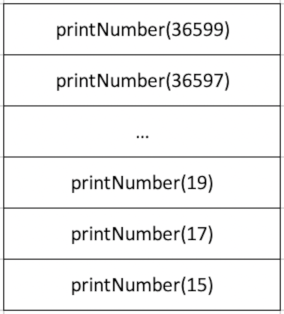
\includegraphics{images/h2/java_call_stack.png}
\caption{Java call stack}
\label{fig:call_stack}
\end{figure}


\subsubsection{OutOfMemoryError}

\begin{lstlisting}
public class DemoOutOfMemory {

	private void generateOutOfMemory() {
		Long maxMemory = Runtime.getRuntime().maxMemory();
		System.out.println(maxMemory);

		int[] matrix = new int[(int) (maxMemory + 1)];
		for (int i = 0; i < matrix.length; ++i) {
			matrix[i] = i + 1;
		}
		System.out.println("Matrix filled" + matrix[(int)(Math.random() * 100)]);

	}

	public static void main(String[] args) {
		DemoOutOfMemory doom = new DemoOutOfMemory();
		doom.generateOutOfMemory();
	}
}
\end{lstlisting}

Om de OutOfMemoryError te illustreren maken we een array aan die meer geheugenplaatsen inneemt dan de ruimte die het java programma ter beschikking heeft.

Als je dit programma uitvoert, pas je best het beschikbare geheugen voor het programma aan. Dit doe je door een waarde voor de VM optie -Xmx mee te geven.

\begin{itemize}
\item -Xmssize: Geeft de initi\"ele waarde voor de heap size.
\item -Xmxsize: Geeft de maximale waarde voor heap size.
\end{itemize}

De heap size van een Java programma is de hoeveelheid geheugen dat een Java-programma mag gebruiken om objecten op te slaan.

\begin{verbatim}
67108864
Exception in thread "main" java.lang.OutOfMemoryError: Java heap space
	at be.pxl.ja.DemoOutOfMemory.generateOutOfMemory(DemoOutOfMemory.java:8)
	at be.pxl.ja.DemoOutOfMemory.main(DemoOutOfMemory.java:16)<5 internal calls>
\end{verbatim}
	
\begin{figure}[H]
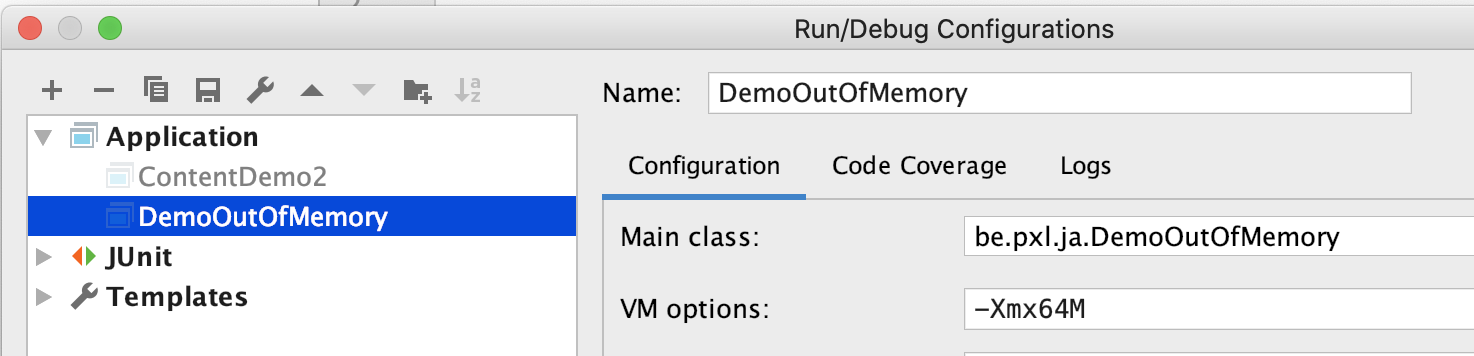
\includegraphics[width=\linewidth]{images/h2/jvm_options_xmx.png}
\caption{Maximum heap size aanpassen}
\label{fig:exceptiono_hierarchy}
\end{figure}

\subsection{Runtime exceptions}

Runtime exceptions zijn exceptions die vaak veroorzaakt worden door logische fouten in het programma.Typische voorbeelden van runtime exceptions zijn ArrayIndexOutOfBoundsException, NullPointerException en IllegalArgumentException. Vaak moet je ze niet afhandelen, maar moet je ervoor zorgen dat je de bug in je code oplost. Ook hier zijn onze unit testen heel belangrijk. Door goede unit testen te schrijven ga je runtime exceptions in je code opmerken en kunnen oplossen.

\begin{lstlisting}
public class Demo {

	public static void main(String[] args) {
		String tekst = "abc";
		System.out.println(tekst.repeat(-5));
	}
}
\end{lstlisting}

\begin{verbatim}
Exception in thread "main" java.lang.IllegalArgumentException: count is negative: -5
	at java.base/java.lang.String.repeat(String.java:3586)
	at be.pxl.ja.streamingservice.Demo.main(Demo.java:5)
\end{verbatim}

\begin{oefening}

\begin{lstlisting}
public class StreamingService {

	private List<Account> accounts;

	public void addAccount(Account account) {
		accounts.add(account);
	}
}
\end{lstlisting}

Welke exception doet zich voor zodra je voor een object van de klasse StreamingService de methode addAccount() aanroept? Waarom treedt die exception op?
\end{oefening}

Wanneer je programma gebruikmaakt van gegevens die door de gebruiker worden ingevoerd, moet je er altijd rekening mee houden dat de gebruiker foutieve gegevens kan ingeven. Deze foutieve gegevens kunnen aanleiding geven tot runtime exceptions. Ook hier moet je steeds anticiperen op de mogelijke input die de gebruiker kan invoeren. 


\begin{lstlisting}
public class ElementInArray {

	public static void main(String[] args) {
		String[] elements = { "H", "He", "Li", "Be", "B", "C", "N", "O", "F", "Ne" };

		Scanner scanner = new Scanner(System.in);
		
		// OPLOSSING 1
		System.out.println("Kies een nummer: ");
		int chosen = scanner.nextInt();
		if (chosen < elements.length) {
			System.out.println(elements[chosen]);
		} else {
			System.out.println("U koos een verkeerd nummer.");
		}

	    // OPLOSSING 2
		System.out.println("Kies een nummer: ");
		chosen = scanner.nextInt();
		try {
			System.out.println(elements[chosen]);
		} catch (ArrayIndexOutOfBoundsException e) {
			System.out.println("U koos een verkeerd nummer.");
		}
	}
}
\end{lstlisting}

In bovenstaand codevoorbeeld gaat onze voorkeur uit naar oplossing 1 waarbij de ingevoerde waarde wordt gecontroleerd vooraleer het element uit de array wordt benaderd. Deze code is makkelijker leesbaar en onderhoudbaar.

\begin{oefening}
Maak een programma dat de geboortedatum vraagt als input. Vervolgens berekent het programma hoeveel dagen het nog duurt vooraleer je jarig bent. Gebruik de methode parse() uit de klasse LocalDateTime om van de input van de gebruiker een LocalDateTime-object te maken. Welke exception kan optreden? Blijf input vragen totdat de gebruiker een correcte datum heeft ingegeven.
\end{oefening}


\subsection{Checked exceptions}

Wanneer je in java een methode aanroept, kan het voorkomen dat je direct een compileerfout voorgeschoteld krijgt. Het kan namelijk zijn dat java reeds anticipeert op mogelijke problemen en je dwingt om rekening te houden met het scenario dat er iets mis kan gaan. De compileerfout raakt pas opgelost wanneer je het afhandelen van de exception netjes programmeert.

Kijk eens naar onderstaand voorbeeld uit de streaming service.
We gebruiken hier de klasse MessageDigest uit JDK. Message digests zijn functies waarmee we voor input-data van willekeurige lengte een hash-waarde met een vaste lengte kunnen berekenen.  Als je de hash-waarde kent, kan je hieruit de input-data niet afleiden. We gebruiken dit om een paswoord bij te houden in een Account-object. We willen absoluut vermijden dat paswoorden in een leesbaar formaat in onze objecten worden bijgehouden.

Om een message digest te berekenen in Java moet je eerst de static methode getInstance() aanroepen met als parameter het door jouw gekozen algoritme. In dit voorbeeld wordt er gekozen voor MD5. Je ziet dat de lijn code, ondanks het feit dat alles correct is geschreven, toch rood wordt onderlijnd. Dat komt omdat de methode getInstance() een exception kan opgooien die we verplicht moeten afhandelen.

\begin{oefening}
Open de documentatie van de klasse MessageDigest en bekijk de uitleg voor de static methode getInstance(). Kan je hier zien welke exceptions er kunnen voorkomen?
\end{oefening}

\begin{figure}[H]
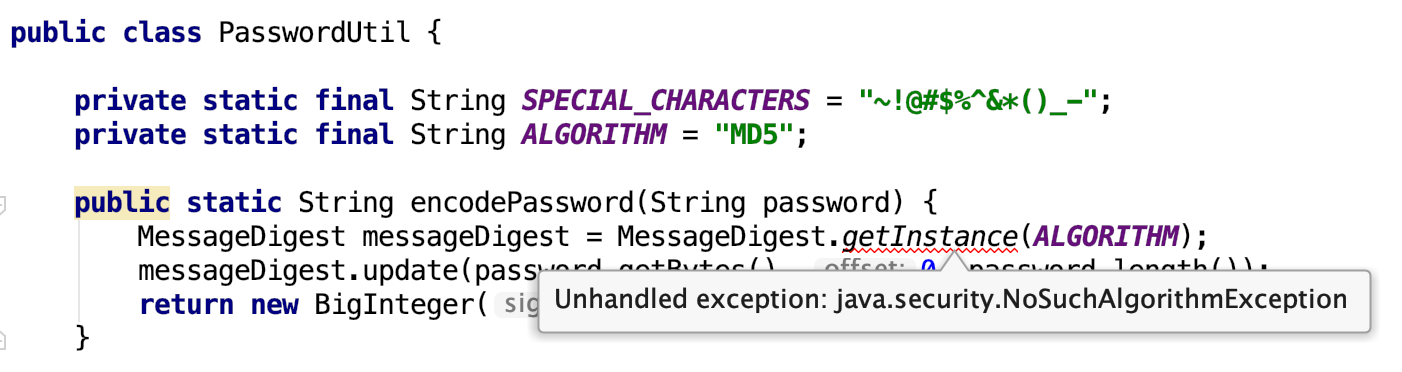
\includegraphics[width=\linewidth]{images/h2/no_such_algorithm_exception.png}
\caption{Een checked exception: NoSuchAlgorithmException}
\label{fig:no_such_algorithm}
\end{figure}

Deze compileerfout wordt veroorzaakt omdat de exception-klasse NoSuchAlgorithmException een checked exception is. Dit betekent dat het aanroepen van de methode die de exception gooit een compileerfout zal geven, omdat er geen code is toegevoegd om correct met de  exception om te gaan.
Er zijn 2 mogelijke oplossingen om deze compileerfout aan te pakken. Ofwel vang de exception op en handel je ze af in de methode encodePassword(), ofwel voeg je in de signatuur van de methode encodePassword() toe dat je de methode toelaat om een NoSuchAlgorithmException op te werpen. We geven nu eerst een voorbeeld van hoe je de exception kan opvangen en afhandelen. 

\begin{lstlisting}
import be.pxl.ja.streamingservice.util.PasswordUtil;

public class Account {
	private String email;
	private String password;

	public Account(String email, String password) {
		this.email = email;
		setPassword(password);
	}

	public String getEmail() {
		return email;
	}

	public void setEmail(String email) {
		this.email = email;
	}

	public boolean verifyPassword(String password) {
		return PasswordUtil.isValid(password, this.password);
	}

	public void setPassword(String password) {
		this.password = PasswordUtil.encodePassword(password);
	}
}
\end{lstlisting}

\begin{lstlisting}
import java.math.BigInteger;
import java.security.MessageDigest;
import java.security.NoSuchAlgorithmException;

public class PasswordUtil {

	private static final String ALGORITHM = "MD5";

	public static String encodePassword(String password) {
		MessageDigest messageDigest = null;
		try {
			messageDigest = MessageDigest.getInstance(ALGORITHM);
		} catch (NoSuchAlgorithmException e) {
			return null;
		}
		messageDigest.update(password.getBytes(), 0, password.length());
		return new BigInteger(1, messageDigest.digest()).toString(16);
	}

	public static boolean isValid(String providedPassword, String securedPassword) {
		return encodePassword(providedPassword).equals(securedPassword);
	}
}
\end{lstlisting}


\begin{lstlisting}
import be.pxl.ja.streamingservice.model.Account;

public class CheckedExceptionDemo {

	public static void main(String[] args) {
		Account newAccount = new Account("daffy@duckstad.be", "daffy123!");
		System.out.println(newAccount.verifyPassword("daffy123"));
		System.out.println(newAccount.verifyPassword("daffy123!"));
	}
}
\end{lstlisting}

Het algoritme ``MD5'' is een geldige waarde voor de parameter algorithm en je krijgt een probleemloos verloop van je programma. Maar een programmeur die zich vergist en de constante ALGORITHM in de klasse PasswordUtil de waarde ``MD4'' geeft zal een probleem veroorzaken.

\begin{verbatim}
Exception in thread "main" java.lang.NullPointerException
	at be.pxl.ja.streamingservice.util.PasswordUtil.isValid(PasswordUtil.java:24)
	at be.pxl.ja.streamingservice.model.Account.verifyPassword(Account.java:37)
	at be.pxl.ja.streamingservice.CheckedExceptionDemo.main(CheckedExceptionDemo.java:9)
\end{verbatim}

\begin{figure}[H]
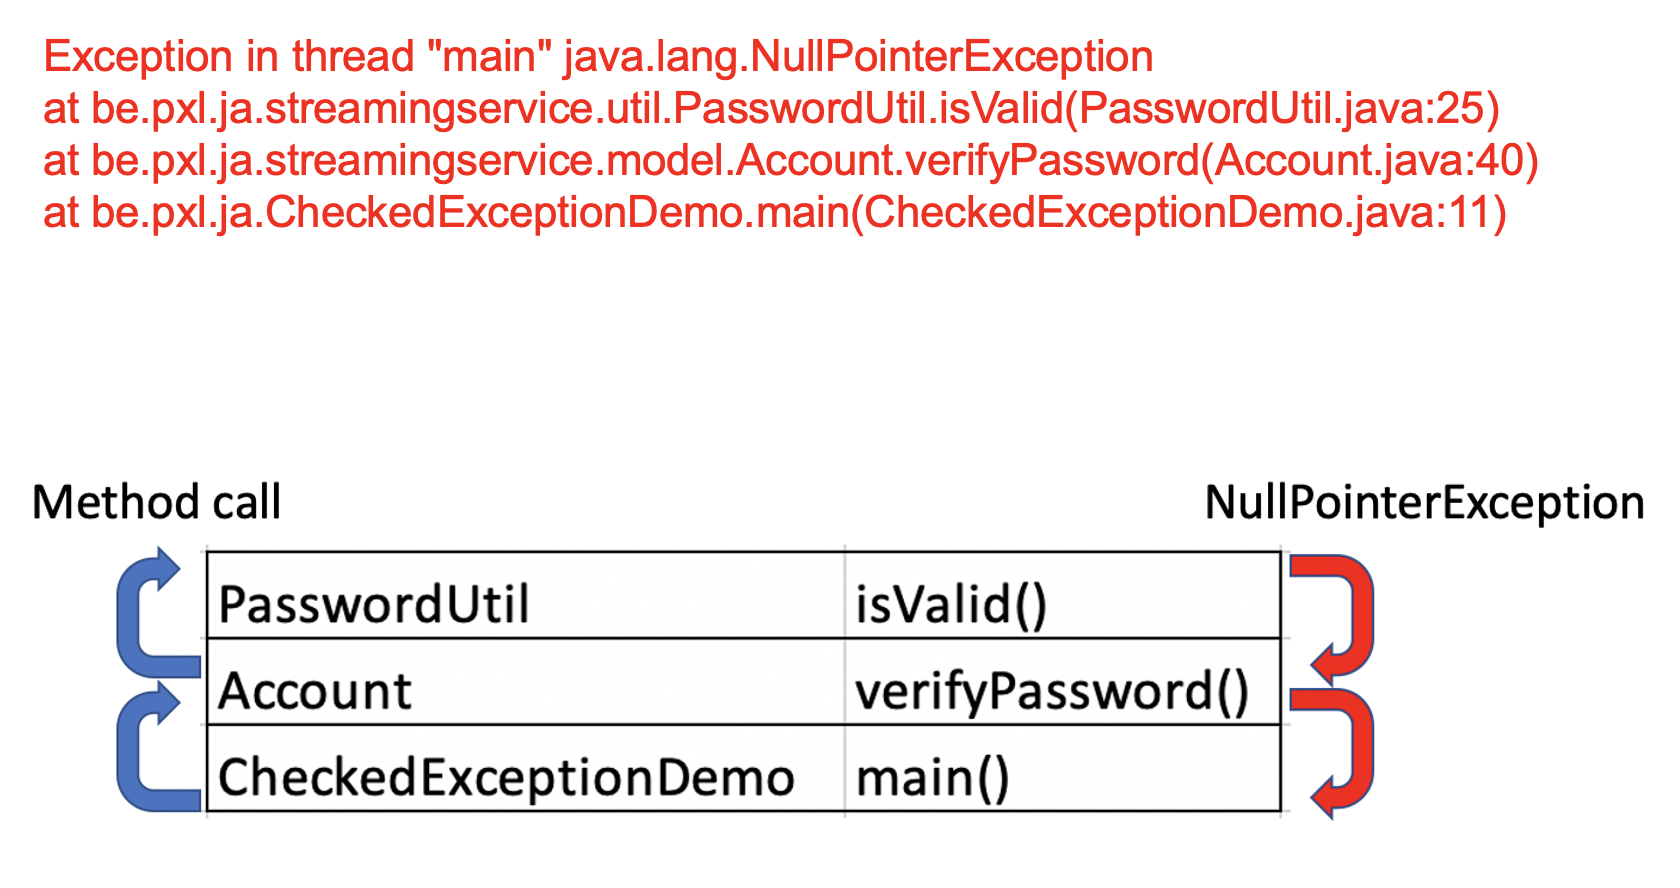
\includegraphics[width=\linewidth]{images/h2/exception_call_stack.png}
\caption{Method call stack}
\label{fig:method_call_stack}
\end{figure}

De NoSuchAlgorithmException wordt afgehandeld door null te geven als returnwaarde van de methode encodePassword.  Hierdoor wordt het probleem pas opgemerkt op het ogenblik dat we de methode isValid van de klasse PasswordUtil gebruiken. De informatie dat het foute algoritme werd meegegeven is momenteel volledig verloren gegaan. Daarom wordt altijd aangeraden om exceptions die zich voordoen in je programma bij te houden in logbestanden. Het gebruik van logbestanden valt buiten de scope van deze cursus. Als alternatief voor het loggen van exceptions zullen we in deze cursus de stacktrace van de exception tonen in de console.

\begin{lstlisting}
import java.math.BigInteger;
import java.security.MessageDigest;
import java.security.NoSuchAlgorithmException;

public class PasswordUtil {

	private static final String ALGORITHM = "MD4";

	public static String encodePassword(String password) {
		MessageDigest messageDigest = null;
		try {
			messageDigest = MessageDigest.getInstance(ALGORITHM);
		} catch (NoSuchAlgorithmException e) {
			e.printStackTrace();
			return null;
		}
		messageDigest.update(password.getBytes(), 0, password.length());
		return new BigInteger(1, messageDigest.digest()).toString(16);
	}

	public static boolean isValid(String providedPassword, String securedPassword) {
		return encodePassword(providedPassword).equals(securedPassword);
	}
}
\end{lstlisting}
 
Door de stacktrace te tonen in de console raken we geen cruciale informatie kwijt.

\begin{verbatim}
java.security.NoSuchAlgorithmException: MD4 MessageDigest not available
	at java.base/sun.security.jca.GetInstance.getInstance(GetInstance.java:159)
	at java.base/java.security.Security.getImpl(Security.java:700)
	at java.base/java.security.MessageDigest.getInstance(MessageDigest.java:177)
	at be.pxl.ja.streamingservice.util.PasswordUtil.encodePassword(PasswordUtil.java:15)
	at be.pxl.ja.streamingservice.model.Account.setPassword(Account.java:45)
	at be.pxl.ja.streamingservice.model.Account.<init>(Account.java:16)
	at be.pxl.ja.streamingservice.CheckedExceptionDemo.main(CheckedExceptionDemo.java:8)
java.security.NoSuchAlgorithmException: md4 MessageDigest not available
	at java.base/sun.security.jca.GetInstance.getInstance(GetInstance.java:159)
	at java.base/java.security.Security.getImpl(Security.java:700)
	at java.base/java.security.MessageDigest.getInstance(MessageDigest.java:177)
	at be.pxl.ja.streamingservice.util.PasswordUtil.encodePassword(PasswordUtil.java:15)
	at be.pxl.ja.streamingservice.util.PasswordUtil.isValid(PasswordUtil.java:25)
	at be.pxl.ja.streamingservice.model.Account.verifyPassword(Account.java:37)
	at be.pxl.ja.streamingservice.CheckedExceptionDemo.main(CheckedExceptionDemo.java:9)
Exception in thread "main" java.lang.NullPointerException
	at be.pxl.ja.streamingservice.util.PasswordUtil.isValid(PasswordUtil.java:25)
	at be.pxl.ja.streamingservice.model.Account.verifyPassword(Account.java:37)
	at be.pxl.ja.streamingservice.CheckedExceptionDemo.main(CheckedExceptionDemo.java:9)
\end{verbatim}

Opnieuw zie je het belang van unit testen. Een foute waarde voor het gekozen algoritme ga je al heel snel opmerken en herstellen als je unit testen schrijft voor de methoden encodePassword() en isValid().

In dit voorbeeld is het eigenlijk aangewezen om de exception niet af te handelen. Een alternatief is dat we de methode encodePassword() toelaten om de exception, als die zich voordoet, gewoon verder door te geven (gooien).
Hierdoor komt de exception dus terecht op de plaatsen waar je de methode encodePassword() gaat aanroepen en moet je op die plaatsen afhandeling voorzien. Je kan er dus voor kiezen om de checked exception NoSuchAlgorithmException helemaal mee te sleuren doorheen je applicatie tot aan de main()-methode.

\begin{lstlisting}
import java.math.BigInteger;
import java.security.MessageDigest;
import java.security.NoSuchAlgorithmException;

public class PasswordUtil {

	private static final String ALGORITHM = "MD5";

	public static String encodePassword(String password) throws NoSuchAlgorithmException {
		MessageDigest messageDigest = MessageDigest.getInstance(ALGORITHM);
		messageDigest.update(password.getBytes(), 0, password.length());
		return new BigInteger(1, messageDigest.digest()).toString(16);
	}

	public static boolean isValid(String providedPassword, String securedPassword) throws NoSuchAlgorithmException {
		return encodePassword(providedPassword).equals(securedPassword);
	}
}
\end{lstlisting}

\begin{lstlisting}
import java.security.NoSuchAlgorithmException;
import java.util.ArrayList;
import java.util.List;

public class Account {
	private String email;
	private String password;

	public Account(String email, String password) throws NoSuchAlgorithmException {
		this.email = email;
		setPassword(password);
	}

	public String getEmail() {
		return email;
	}

	public void setEmail(String email) {
		this.email = email;
	}

	public boolean verifyPassword(String password) throws NoSuchAlgorithmException {
		return PasswordUtil.isValid(password, this.password);
	}

	public void setPassword(String password) throws NoSuchAlgorithmException {
		this.password = PasswordUtil.encodePassword(password);
	}
}
\end{lstlisting}

\begin{lstlisting}
import be.pxl.ja.streamingservice.model.Account;
import java.security.NoSuchAlgorithmException;

public class CheckedExceptionDemo {

	public static void main(String[] args) throws NoSuchAlgorithmException {
		Account newAccount = new Account("daffy@duckstad.be", "daffy123!");
		System.out.println(newAccount.verifyPassword("daffy123"));
		System.out.println(newAccount.verifyPassword("daffy123!"));
	}
}
\end{lstlisting}

Je ziet dat nu bij de signatuur van verschillende methoden ``throws NoSuchAlgorithmException'' verschijnt.
Regelmatig verschijnen er artikels met titels als ``Checked exceptions: Java’s biggest mistake'' en ``Checked Exceptions are Evil'' om het gebruik van checked exceptions te ontmoedigen. 

Een laatste en nette oplossing is om de NoSuchAlgorithmException the \textbf{wrappen}  in een runtime exception bijv. een IllegalArgumentException.

\begin{lstlisting}
import java.math.BigInteger;
import java.security.MessageDigest;
import java.security.NoSuchAlgorithmException;

public class PasswordUtil {

	private static final String ALGORITHM = "MD4";

	public static String encodePassword(String password) {
		MessageDigest messageDigest = null;
		try {
			messageDigest = MessageDigest.getInstance(ALGORITHM);
		} catch (NoSuchAlgorithmException e) {
			throw new IllegalArgumentException(e);
		}
		messageDigest.update(password.getBytes(), 0, password.length());
		return new BigInteger(1, messageDigest.digest()).toString(16);
	}

	public static boolean isValid(String providedPassword, String securedPassword) {
		return encodePassword(providedPassword).equals(securedPassword);
	}
}
\end{lstlisting}

Bij het uitvoeren van de methode encodePassword() met een foutief algoritme krijg je dan een runtime exception.

\begin{verbatim}
Exception in thread "main" java.lang.IllegalArgumentException: java.security.NoSuchAlgorithmException: MD4 MessageDigest not available
	at be.pxl.ja.streamingservice.util.PasswordUtil.encodePassword(PasswordUtil.java:17)
	at be.pxl.ja.streamingservice.model.Account.setPassword(Account.java:48)
	at be.pxl.ja.streamingservice.model.Account.<init>(Account.java:18)
	at be.pxl.ja.CheckedExceptionDemo.main(CheckedExceptionDemo.java:10)
	at java.base/jdk.internal.reflect.NativeMethodAccessorImpl.invoke0(Native Method)
	at java.base/jdk.internal.reflect.NativeMethodAccessorImpl.invoke(NativeMethodAccessorImpl.java:62)
	at java.base/jdk.internal.reflect.DelegatingMethodAccessorImpl.invoke(DelegatingMethodAccessorImpl.java:43)
	at java.base/java.lang.reflect.Method.invoke(Method.java:564)
	at com.intellij.rt.execution.application.AppMainV2.main(AppMainV2.java:131)
Caused by: java.security.NoSuchAlgorithmException: MD4 MessageDigest not available
	at java.base/sun.security.jca.GetInstance.getInstance(GetInstance.java:159)
	at java.base/java.security.Security.getImpl(Security.java:700)
	at java.base/java.security.MessageDigest.getInstance(MessageDigest.java:177)
	at be.pxl.ja.streamingservice.util.PasswordUtil.encodePassword(PasswordUtil.java:15)
	... 8 more
\end{verbatim}

\section{Multi-catch blok en finally}

\begin{lstlisting}
import java.util.Scanner;

public class MultiCatchBlockDemo {

	public static void main(String[] args) {
		Scanner scanner = new Scanner(System.in);
		System.out.println("Kies een positie: ");
		int positie = scanner.nextInt();
		System.out.println("Kies een deler: ");
		int deler = scanner.nextInt();
		try {
			int getallen[] = new int[10];
			getallen[positie] = 30 / deler;
		} catch (ArrayIndexOutOfBoundsException e) {
			System.out.println("Je moet een positie kiezen tussen 0 en 9.");
		} catch (Exception e) {
			System.out.println(e.getMessage());
		} finally {
			System.out.println("Je koos positie " + positie);
		}
		System.out.println("Start je het programma nog een keer.");
	}
}
\end{lstlisting}

Een try-blok kan gevolgd worden door \'e\'en of meerder catch-blokken.
Wanneer een exception optreedt zal bij het eerste catch-blok gestart worden. Indien onze exception een instantie is van de opgevangen exception  (instanceof) dan zal dat catch-blok uitgevoerd worden en worden de volgende catch-blokken niet meer bekeken. Indien de exception geen instantie is van de opgevangen exception dan wordt er verder gekeken naar de volgende catch-blokken tot een overeenkomstig catch-blok worden gevonden. Indien er geen catch-blok wordt gevonden zal de runtime-exception doorstromen naar de aanroepende methode.

De volgorde van de catch-blokken is van belang. ArrayIndexOutOfBoundsException is een subklasse van Exception. Als we eerst een catch-blok aanmaken voor de superklasse en pas daarna een catch-blok voor de subklasse zou het tweede catch-blok ``onbereikbaar'' zijn. Het eerste catch-blok gaat de exception reeds kunnen afhandelen. Code die onbereikbaar is (unreachable code) wordt opgemerkt door de compiler wat resulteert in een compileerfout van je code.

\begin{oefening}
Wissel beide catch-blokken eens van plaats in bovenstaande code.
\end{oefening}

Het finally-blok tenslotte is een codeblok dat altijd wordt uitgevoerd: of er nu een exception optreedt of niet. Zelfs als er een exception optreedt en die niet kan worden afgehandeld door een catch-blok, zal toch het finally-blok uitgevoerd worden.

\begin{oefening}
Test de werking van het finally-blok eens uit met bovenstaand programma MultiCatchBlockDemo. Verwijder het tweede catch-blok eens en veroorzaak een deling door 0. Wat gebeurt er?
\end{oefening}

Indien je dezelfde code hebt om verschillende exceptions af te handelen, mag je exceptions combineren in een catch-block. Zo zal het catch-blok in onderstaand voorbeeld zowel ArrayIndexOutOfBoundsExceptions als ArithmeticExceptions afhandelen.

\begin{lstlisting}
public class MultipleCatches {

	public static void main(String[] args) {
		Scanner scanner = new Scanner(System.in);
		System.out.println("Kies een positie: ");
		int positie = scanner.nextInt();
		System.out.println("Kies een deler: ");
		int deler = scanner.nextInt();
		try {
			int getallen[] = new int[10];
			getallen[positie] = 30 / deler;
		} catch (ArrayIndexOutOfBoundsException | ArithmeticException e) {
			System.out.println(e.getMessage());
		}
		System.out.println("Start je het programma nog een keer.");
	}
}
\end{lstlisting}

\section{Zelf exceptions opgooien}
We willen gaan controleren dat de gebruikers van onze streaming service enkel geldige kredietkaartnummers invullen. Daarom maken we een aparte klasse CreditCardNumber. We gaan ervoor zorgen dat objecten van de klasse CreditCardNumber nooit ongeldige gegevens bevatten. Wanneer je een object van de klasse CreditCardNumber probeert aan te maken met ongeldige gegevens zal er een IllegalArgumentException gegooid worden.

We laten 2 types van kredietkaarten toe: VISA en MASTERCARD. Kaartnummers van VISA-kaarten starten altijd met het nummer 5, kaartnummers van MASTERCARD-kaarten starten altijd met 4.
Verder wordt ook gecontroleerd dat de kaartnummers bestaan uit 16 cijfers. Bestudeer de klasse CreditCardNumber.

\begin{lstlisting}
public class CreditCardNumber {
	private static final int LENGTH = 16;
	private static final int CVC_LENGTH = 3;

	private CreditCardType creditCardType;
	private String number;
	private String cvc;

	public CreditCardNumber(String number, String cvc) {
		if (!isNumeric(number) || number.length() != LENGTH) {
			throw new IllegalArgumentException("A card number must have " + LENGTH + " digits.");
		}
		creditCardType = getCreditCardType(number);
		if (creditCardType == null) {
			throw new IllegalArgumentException("This is not a valid credit card.");
		}
	}

	private boolean isNumeric(String text) {
		if (text == null || text.length() == 0) {
			return false;
		}
		try {
			Long.parseLong(text);
			return true;
		} catch (NumberFormatException e) {
			return false;
		}
	}

	private CreditCardType getCreditCardType(String number) {
		for (CreditCardType cardType : CreditCardType.values()) {
			if (cardType.getFirstNumber() == Integer.parseInt(number.substring(0, 1))) {
				return cardType;
			}
		}
		return null;
	}
}
\end{lstlisting} 

Natuurlijk gaan we de constructor van onze nieuwe klasse CreditCardNumber ook grondig testen.  Wanneer we dus foutieve waarden meegeven aan de constructor gaan we moeten verifi\"eren dat de IllegalArgumentException wordt opgegooid.

Hier is alvast een eenvoudig voorbeeld om te tonen hoe de methode assertThrows van de klasse Assertions in junit werkt.

\begin{lstlisting}
@Test
void testExpectedException() {
  Assertions.assertThrows(NumberFormatException.class, () -> {
    Integer.parseInt("One");
  });
}
\end{lstlisting}

De assertThrows() verwacht dat een NumberFormatException zal worden opgegooid. Omdat de string ``One'' een ongeldige waarde is zal de NumberFormatException ook effectief gegooid worden en zal de test dus slagen.

Nu zie je een aantal testen om onze constructor van de klasse CreditCardNumber te testen. Bestudeer de testen grondig.


\begin{lstlisting}
import org.junit.jupiter.api.Test;

import static org.junit.jupiter.api.Assertions.assertEquals;
import static org.junit.jupiter.api.Assertions.assertThrows;

public class CreditCardNumberTest {

	@Test
	public void validVisaCard() {
		CreditCardNumber creditCardNumber = new CreditCardNumber("4321876532147654", "123");

		assertEquals(CreditCardType.VISA, creditCardNumber.getType());
		assertEquals("123", creditCardNumber.getCvc());
		assertEquals("4321876532147654", creditCardNumber.getNumber());
	}

	@Test
	public void validVisaCardWithBlanks() {
		CreditCardNumber creditCardNumber = new CreditCardNumber("  43218 76532 1476 54  ", " 1 2 3 ");

		assertEquals(CreditCardType.VISA, creditCardNumber.getType());
		assertEquals("123", creditCardNumber.getCvc());
		assertEquals("4321876532147654", creditCardNumber.getNumber());
	}

	@Test
	public void validMasterCard() {
		CreditCardNumber creditCardNumber = new CreditCardNumber("5321876532147654", "123");

		assertEquals(CreditCardType.MASTERCARD, creditCardNumber.getType());
		assertEquals("123", creditCardNumber.getCvc());
		assertEquals("5321876532147654", creditCardNumber.getNumber());
	}

	@Test
	public void validMasterCardWithBlanks() {
		CreditCardNumber creditCardNumber = new CreditCardNumber("  53218 76532 1476 54  ", " 1 2 3 ");

		assertEquals(CreditCardType.MASTERCARD, creditCardNumber.getType());
		assertEquals("123", creditCardNumber.getCvc());
		assertEquals("5321876532147654", creditCardNumber.getNumber());
	}

	@Test
	public void throwsInvalidArgumentExceptionWhenNumberTooShort() {
		assertThrows(IllegalArgumentException.class, () -> {
			new CreditCardNumber("  53218 76532 1476  ", " 1 2 3 ");
		});
	}

	@Test
	public void throwsInvalidArgumentExceptionWhenNumberTooLong() {
		assertThrows(IllegalArgumentException.class, () -> {
			new CreditCardNumber("  53218 76532 1476 4445  ", " 1 2 3 ");
		});
	}

	@Test
	public void throwsInvalidArgumentExceptionWhenInvalidCardType() {
		assertThrows(IllegalArgumentException.class, () -> {
			new CreditCardNumber("7321876532147654", "123");
		});
	}
}
\end{lstlisting}

\begin{oefening}
Voeg in de constructor van de klasse CreditCardNumber een extra validatie toe voor de CVC (card validation code). De CVC is een getal bestaande uit 3 cijfers.
Pas je unit testen aan. Waarschijnlijk moet je extra unit testen toevoegen om de constructor van de klasse CreditCardNumber te testen.
\end{oefening}


\section{Zelf exception-klassen schrijven}

In de klasse CreditCardNumber hebben we gebruikgemaakt van een bestaande exception uit de JDK. We kunnen ook onze eigen Exception-klassen voorzien.

De klasse PaymentInfo gaan we nu grondig aanpassen door o.a. gebruik te maken van de klasse CreditCardNumber. Daarnaast willen we ook de vervaldatum van de kredietkaart gaan controleren. We willen namelijk dat de kredietkaart nog minstens 1 maand geldig is op het ogenblik dat de betaalgegevens worden ingegeven. Indien de vervaldatum binnen de maand valt, gaan we een InvalidDateException opgooien.

Deze InvalidDateException-klasse bestaat niet in de JDK, dus gaan we hem zelf voorzien. Wanneer je een \textbf{checked exception} wil maken gebruik je de klasse Exception als superklasse van je nieuwe exception. Wanneer je een \textbf{unchecked exception} wil maken gebruik je de klasse RuntimeException als superklasse.

Hier is alvast onze nieuwe exception klasse InvalidDateException. Als je zelf een exception klasse aanmaakt kan je zelf beslissen welke parameters en extra eigenschappen je voorziet in de constructor. Regelmatig wordt ook de afspraak gehanteerd dat er pas een nieuwe exception klasse wordt toegevoegd, indien \'e\'en van de reeds bestaande exception klassen niet eenvoudig hergebruikt kan worden. In ons geval, gaan we de ongeldige datum willen tonen. Om het samenstellen van de foutboodschap te kunnen hergebruiken is het dus zinvol om een InvalidDateException te maken met o.a. de ongeldige datum (LocalDate) als parameter.

\begin{lstlisting}
public class InvalidDateException extends RuntimeException {

	public static final DateTimeFormatter FORMATTER = DateTimeFormatter.ofPattern("dd/MM/yyyy");

	public InvalidDateException(LocalDate incorrectDate, String type, String description) {
		super(FORMATTER.format(incorrectDate) + " is not a valid " + type + ". " + description);
	}
}
\end{lstlisting}

\begin{lstlisting}
import java.time.LocalDate;

public class PaymentInfo {

	private String firstName;
	private String lastName;
	private CreditCardNumber cardNumer;
	private LocalDate expirationDate;

	public String getFirstName() {
		return firstName;
	}

	public void setFirstName(String firstName) {
		this.firstName = firstName;
	}

	public String getLastName() {
		return lastName;
	}

	public void setLastName(String lastName) {
		this.lastName = lastName;
	}

	public void setCardNumer(CreditCardNumber cardNumer) {
		this.cardNumer = cardNumer;
	}

	public LocalDate getExpirationDate() {
		return expirationDate;
	}

	public void setExpirationDate(LocalDate expirationDate) {
		if (LocalDate.now().plusMonths(1).isAfter(expirationDate)) {
			throw new InvalidDateException(expirationDate, "expirationDate", "Must be valid for at least 1 month.");
		}
		this.expirationDate = expirationDate;
	}
}
\end{lstlisting}

We gaan deze  methode setExpirationDate nu ook grondig testen.

\begin{lstlisting}
import org.junit.jupiter.api.BeforeEach;
import org.junit.jupiter.api.Test;

import java.time.LocalDate;

import static org.junit.jupiter.api.Assertions.assertEquals;
import static org.junit.jupiter.api.Assertions.assertNotNull;
import static org.junit.jupiter.api.Assertions.assertThrows;

public class PaymentInfoSetExpirationDateTest {

	private PaymentInfo paymentInfo;

	@BeforeEach
	public void init() {
		paymentInfo = new PaymentInfo();
	}

	@Test
	public void throwsInvalidDateExceptionWhenExpirationDayWithinOneMonth() {
		LocalDate withinOneMonth = LocalDate.now().plusMonths(1).minusDays(1);
		assertThrows(InvalidDateException.class, () -> paymentInfo.setExpirationDate(withinOneMonth));
	}

	@Test
	public void expirationDayWithinExactlyOneMonthIsAllowed() {
		LocalDate exactlyOneMonth = LocalDate.now().plusMonths(1);
		paymentInfo.setExpirationDate(exactlyOneMonth);

		assertNotNull(paymentInfo.getExpirationDate());
		assertEquals(exactlyOneMonth, paymentInfo.getExpirationDate());
	}

	@Test
	public void expirationDayOverOneMonthIsAllowed() {
		LocalDate overOneMonth = LocalDate.now().plusMonths(1).plusDays(1);
		paymentInfo.setExpirationDate(overOneMonth);

		assertNotNull(paymentInfo.getExpirationDate());
		assertEquals(overOneMonth, paymentInfo.getExpirationDate());
	}

}
\end{lstlisting} 

\begin{oefening}
Schrijf ook een kort programma waarin je de InvalidDateException veroorzaakt. Vang de exception op en toon de foutboodschap (message)?
\end{oefening}

\begin{oefening}
In de klasse Profile willen we ook de waarde van de geboortedatum controleren. Zorg ervoor dat er nooit een waarde die in de toekomst ligt als geboortedatum wordt ingevuld via de setter (setDateOfBirth). Indien dit wel gebeurt gooi een een InvalidDateException op. Schrijf unit testen om de methode setDateOfBirth uit de klasse Profile grondig te testen.
\end{oefening}
 
 \begin{figure}[H]
  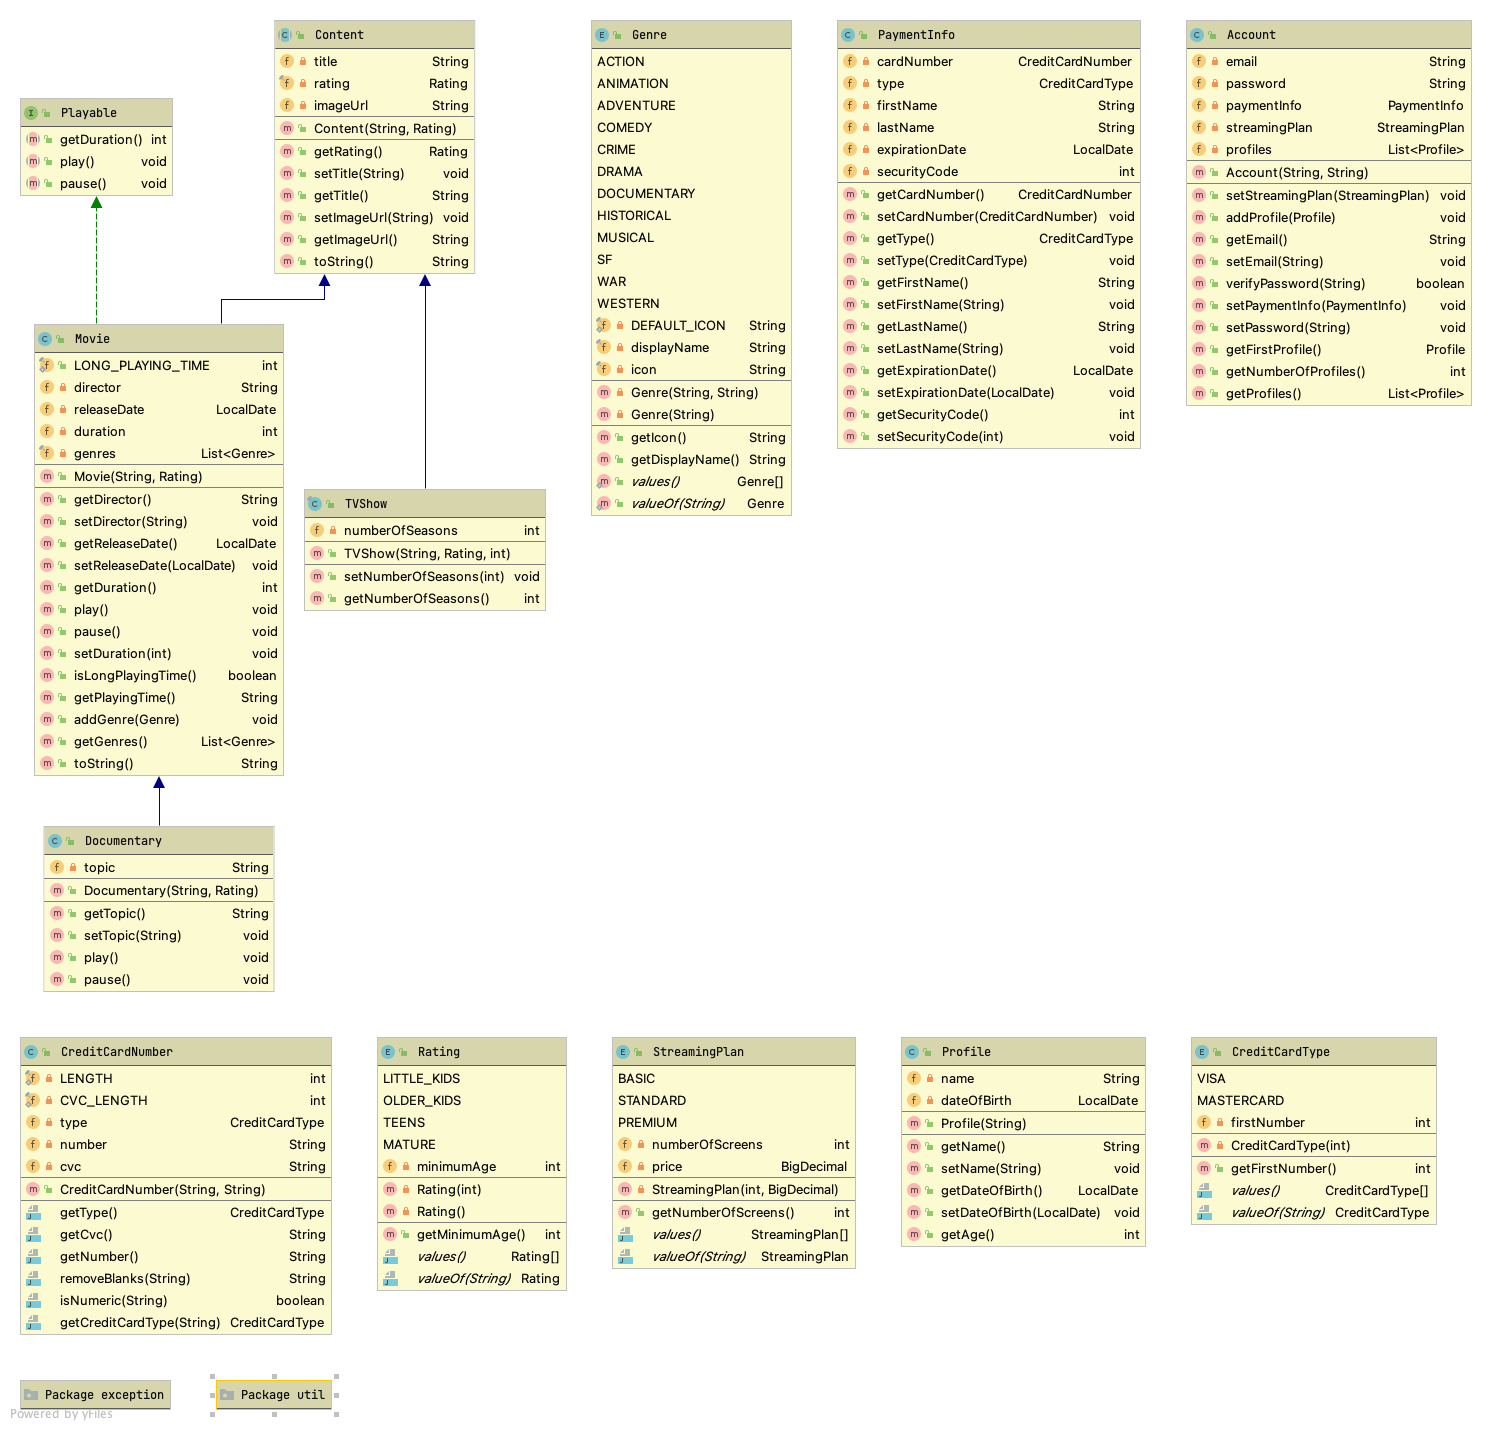
\includegraphics[width=\linewidth]{images/klassendiagram/diagram_H3.png}
  \caption{Klassendiagram}
  \label{fig:klassendiagram}
\end{figure}
 
\begin{remark}
  Meer weten over exception handling, kijk op pluralsight: \url{https://app.pluralsight.com/library/courses/java-fundamentals-exception-handling}
\end{remark}


\chapter{Collections}

\begin{summary}
De programma's die we ontwikkelen hebben gegevens nodig. Denk bijvoorbeeld aan de deelnemers van een wedstrijd, temperaturen voor plaatsen en tijdstippen, uurrooster van een klasgroep,... Deze gegevens moeten door het programma worden onthouden. Om dit mogelijk te maken gebruiken we datastructuren. Je hebt reeds kennisgemaakt met arrays en de klasse ArrayList. Je merkte ongetwijfeld dat de ArrayList flexibeler is dan de array, omdat je geen maximale grootte moet meegeven bij creatie. 

Java groepeert zijn belangrijkste datastructuren in het Java Collections framework. Daarnaast voorziet de API handige functionaliteit zoals het opzoeken, sorteren, toevoegen en andere manipulaties van de gegevens.
\end{summary}


\section{Het Java Collections Framework}

Het Java Collections framework voorziet functionaliteit om verzamelingen van objecten te maken en om handelingen of manipulaties op deze verzamelingen uit te voeren. 
Het Java Collections framework bevat:
\begin{itemize}
\item \textbf{Interfaces}: Door gebruik te maken van interfaces kunnen we onze verzamelingen op een uniforme manier manipuleren zonder ons te bekommeren welke concrete implementatie er gebruikt wordt. \textit{java.util.Collection} is de top-interface van het Java Collections framework. Deze interface bevat enkele belangrijke methoden zoals \textit{size()},\textit{add()}, \textit{remove()}, \textit{clear()}. Hierdoor kan je dus bij iedere verzameling objecten toevoegen en verwijderen. Je kan steeds te weten komen hoeveel objecten er in de verzameling zitten. Iedere verzameling kan ook weer leeggemaakt worden.
\item \textbf{Klassen of implementaties}: Voor iedere interface zijn er \'e\'en of meerdere concrete klassen die je in jouw eigen programma's kan gebruiken. De klasse ArrayList is een voorbeeld van zo een klasse.
\item \textbf{Algoritmen}: Zoeken en sorteren zijn 2 belangrijke bewerkingen die je op een verzameling kan uitvoeren. Het Java Collections framework bevat effici\"ente implementaties voor deze algoritmen.
\end{itemize}

\section{Interfaces}

Het Java Collections framework voorziet een beperkt aantal interfaces waarbij iedere interface typische functionaliteit aanbiedt. Zo zal bijvoorbeeld de List interface de methode \textit{E get(int index)} aanbieden die je niet zult terugvinden in de Set of SortedSet interface. De interfaces zijn ook allemaal generiek. Als jij kiest om een List te maken voor String-objecten dan zal de E in de methode \textit{E get(int index)} als String worden ingevuld, als je Integer-object in de List opslaat wordt de E vervangen door Integer. Generics in Java zullen we uitgebreid bestuderen in het volgende hoofdstuk.

\begin{figure}[H]
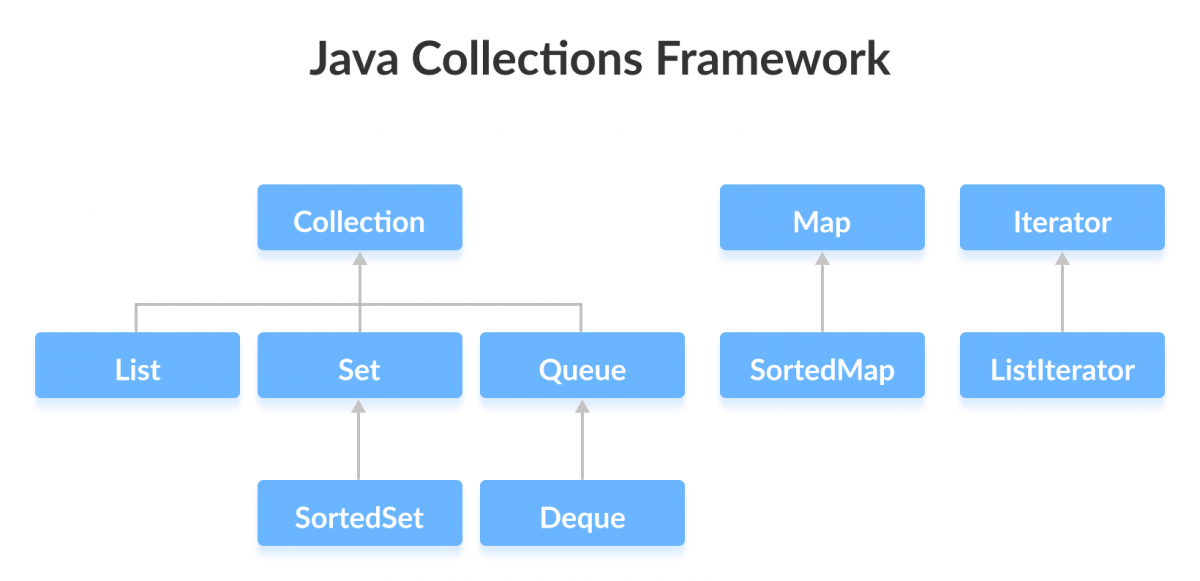
\includegraphics[width=\linewidth]{images/h3/colls-coreInterfaces.png}
\caption{Belangrijkste interfaces}
\label{fig:core_interfaces}
\end{figure}

Om het aantal interfaces in het Java Collections framework eerder beperkt te houden, kan het soms gebeuren dat een concrete klasse er toch voor kiest om een methode uit de interface niet te implementeren. In de plaats zal er dan een UnsupportedOperationException opgegooid worden.

\subsection{Collection}

De interface Collection bevat de essenti\"ele methoden die iedere concrete collection-klasse zal aanbieden.

\begin{oefening}
Neem de documentatie van de interface Collection er even bij en overloop welke methoden je hierin aantreft.
\end{oefening}

\subsection{Set}
In een Set moet ieder element uniek zijn. Dubbele elementen worden niet toegelaten. Een element met de waarde \textit{null} kan je dus maximaal 1 keer in een Set toevoegen.
Enkele voorbeelden voor het gebruik van Sets zijn: de vakken waarvoor je ben ingeschreven aan PXL, een pokerhand, de processen die door je laptop worden uitgevoerd,...
Bij een Set kan je er niet zeker van zijn in welke volgorde de elementen intern worden bijgehouden.

\subsection{List}
In een List moeten de elementen niet uniek zijn. De elementen hebben er wel een vaste volgorde en je kan dan ook kiezen op welke positie in de lijst je iets toevoegt of verwijdert. Je kan ook aan de hand van een positie (index) een element uit de List benaderen.
De temperatuur van een aantal opeenvolgende dagen kan je bijvoorbeeld bijhouden in een List.

\subsection{Queue}
Een Queue is een verzameling waarbij er een rangschikking is waarin de elementen verwerkt moeten worden. De methoden uit de Collection interface worden uitgebreid met extra mogelijkheden om elementen toe te voegen, te verwijderen en op te vragen. Voor elke van deze 3 operaties zijn er 2 methoden voorzien: \'e\'en die een exception zal opwerpen indien de operatie mislukt en een tweede die altijd een return-waarde heeft (bijv. null of false )indien de operatie mislukt. 

\vspace{4mm}
\begin{tabular}{| c | c |  c |} 
\hline
\textbf{Functionaliteit} & \textbf{Met exception} & \textbf{Met return-waarde}\\
\hline
Insert & add(e) & offer(e)\\
Remove & remove() & poll()\\
Examine & element() & peek()\\
\hline
\end{tabular}
\vspace{4mm}

\noindent Bij typsiche Queues zijn de elementen gerangschikt in een FIFO-manier. 
FIFO betekent first-in-first-out en het element dat als eerste werd toegevoegd (met add() of offer()) zal dus ook als eerste verwijderd worden (met remove() of poll()).
Er zijn natuurlijk ook andere implementaties die ervoor kiezen om deze FIFO-regel niet te volgen maar een andere rangschikking te voorzien zoals de PriorityQueue. De spoeddienst van een ziekenhuis zal de pati\"enten niet in een FIFO-volgorde behandelen, maar in een PriorityQueue naargelang de ernst van hun verwondingen.

\subsection{Deque (lees als deck)}

Deque is een verder uitbreiding van Queue en kan daarom eenvoudig gebruikt worden als een FIFO of een LIFO (last-in-first-out) verzameling. Deque staat voor ``double ended queue''.

\vspace{4mm}
\begin{tabular}{| c | c |  c  | c | c |} 
\hline 
 &  \multicolumn{2}{c|}{First element (Head)} &  \multicolumn{2}{c|}{Last element (tail)} \\
\hline
\textbf{Functionaliteit} & \textbf{Met exception} & \textbf{Met return-waarde} & \textbf{Met exception} & \textbf{Met return-waarde} \\
\hline
Insert & addFirst(e)	 & offerFirst(e) &	addLast(e) &	offerLast(e)\\
Remove & removeFirst()	& pollFirst()	& removeLast()	& pollLast() \\
Examine &	getFirst()	& peekFirst()	& getLast() &	peekLast()\\
\hline
\end{tabular}
\vspace{4mm}

\begin{figure}[H]
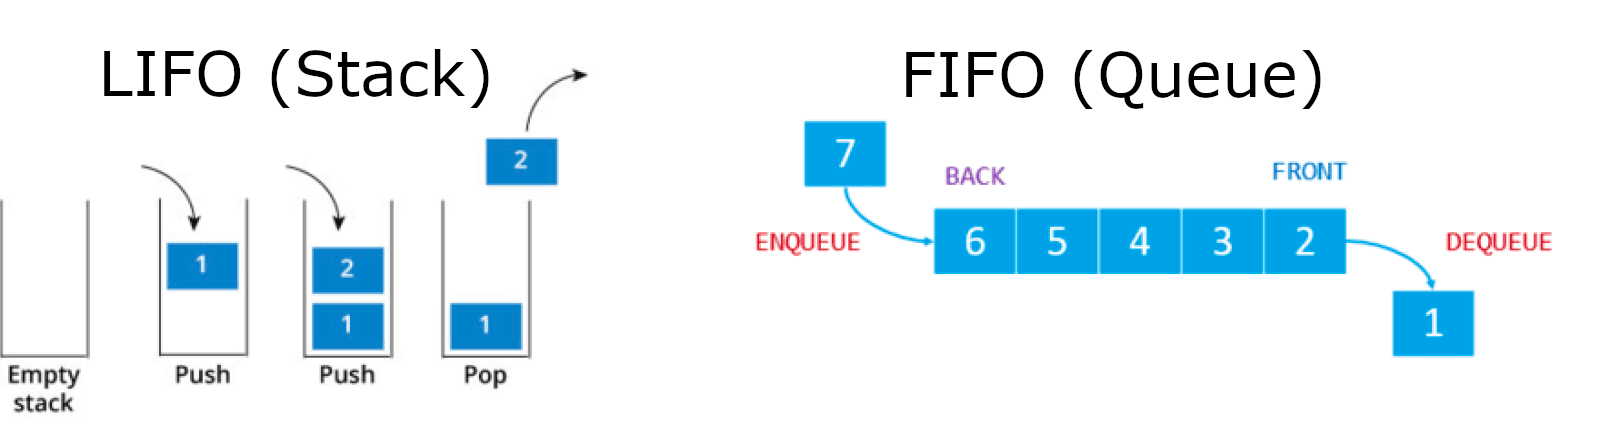
\includegraphics[width=\linewidth]{images/h3/fifo_lifo.png}
\caption{LIFO en FIFO}
\label{fig:fifo_lifo}
\end{figure}

\subsection{Map}

Alle subklassen van Map zijn datastructuren die een key mappen (linken) met een value. Iedere key moet uniek zijn en bij iedere key is er hoogstens \'e\'en value.

\begin{figure}[H]
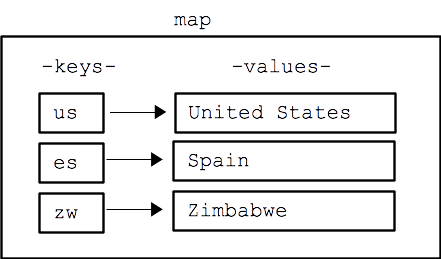
\includegraphics{images/h3/key_value_map1.png}
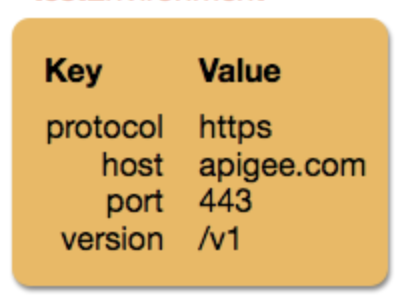
\includegraphics{images/h3/key_value_map2.png}
\caption{Voorbeelden van key-value mappings}
\label{fig:key_value_mappings}
\end{figure}

\section{Concrete klassen}

\begin{figure}[H]
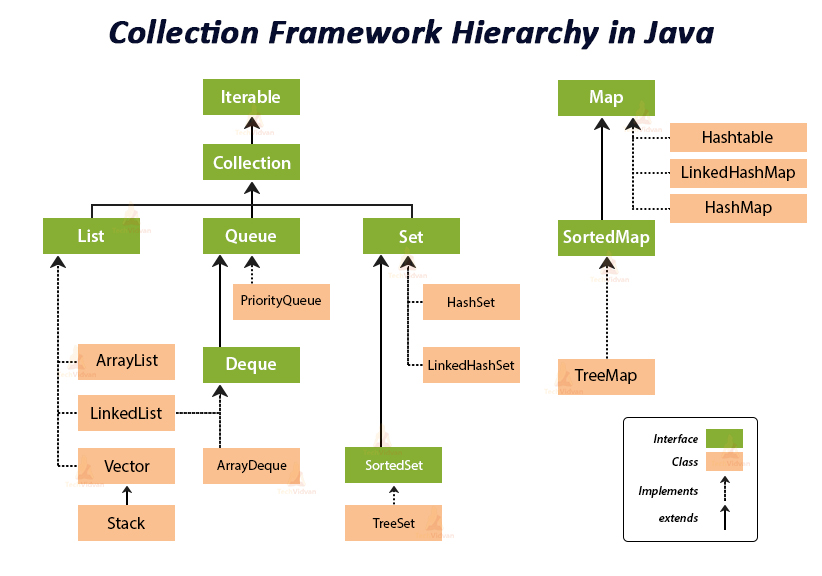
\includegraphics[width=\linewidth]{images/h3/collection-framework-hierarchy-in-java.jpg}
\caption{Java Collection hi\"erarch}
\label{fig:core_classes}
\end{figure}

\begin{figure}[H]
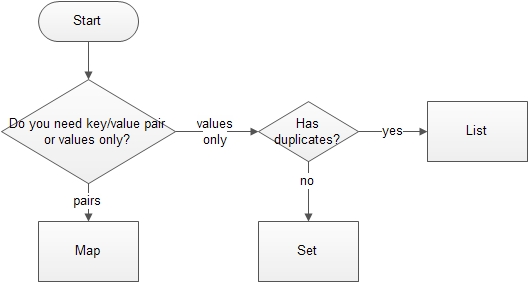
\includegraphics{images/h3/choose-java-collection-interface.jpg}
\caption{Kies een interface}
\label{fig:key_value_mappings}
\end{figure}

\vspace{4mm}
\begin{tabular}{| c | c |  c | c  || c | c |} 
\hline 
\textbf{Interface} & Hash Table & 	Resizable Array	 &	Linked List &	Hash Table + Linked List & Balanced Tree\\
\hline
Set	& HashSet	 	& &	 	&LinkedHashSet & TreeSet \\
List	 & &	ArrayList & 	 	LinkedList	 & & \\
Deque	& &	ArrayDeque	& 	LinkedList	  & &\\
Map	& HashMap	& & 	&	 	LinkedHashMap &TreeMap\\
\hline
\end{tabular}
\vspace{4mm}

\begin{tabular}{|c|c|c|c|c|c|}
\hline
Class & Duplicates? & Null? & Inserted order & Sorted order & Default capacity \\
\hline
ArrayList & \textcolor{green}{Yes} & \textcolor{green}{Yes} &\textcolor{green}{Yes} & \textcolor{red}{No} & 10 \\
LinkedList & \textcolor{green}{Yes} & \textcolor{green}{Yes} &\textcolor{green}{Yes} & \textcolor{red}{No} & 0 \\
HashSet & \textcolor{red}{No} & \textcolor{green}{Yes} &\textcolor{red}{No} & \textcolor{red}{No} & 16 \\
LinkedHashSet & \textcolor{red}{No} & \textcolor{green}{Yes} & \textcolor{green}{Yes}& \textcolor{red}{No} & 16 \\
TreeSet & \textcolor{red}{No} & \textcolor{red}{No} & \textcolor{red}{No} & \textcolor{green}{Yes} & 16 \\
PriorityQueue & \textcolor{green}{Yes} & \textcolor{red}{No} & \textcolor{red}{No} & \textcolor{green}{Yes} & 11 \\
ArrayDeque & \textcolor{green}{Yes} & \textcolor{red}{No} & \textcolor{green}{Yes} & \textcolor{red}{No} & 11 \\
\hline
\end{tabular}
\vspace{4mm}

In Java documentatie en tutorials komen vaak de termen ordered en sorted voor wanneer het gaat over collections. Een collection is ``ordered'' wanneer de elementen een rangschikking hebben. De rangschikking is onafhankelijk van de waarde van de elementen. Een collection is ``sorted'' wanneer de rangschikking ook nog eens afhankelijk is van de waarde van de elementen. 

\section{De klasse ArrayList}

\subsection{Constructor}

De klasse ArrayList heb je al vaak gebruikt. Hier is nog eens een voorbeeld.
We voorzien een klasse ContentRepository: een opslagplaats voor onze Content-objecten. Een object van deze klasse kunnen we gebruiken om een List van Content-objecten aan op te vragen.

\begin{lstlisting}
import java.time.LocalDate;
import java.util.ArrayList;
import java.util.List;

public class ContentRepository {

	private List<Content> contentList;

	public ContentRepository() {
		init();
	}

	private void init() {
		contentList = new ArrayList<>();

		// add initial content to contentList
		Movie theIncredibles = new Movie("The Incredibles", Rating.LITTLE_KIDS);
		theIncredibles.setReleaseDate(LocalDate.of(2004, 10, 27));
		theIncredibles.setImageUrl("the_incredibles.jpeg");
		contentList.add(theIncredibles);

		Documentary planetEarth = new Documentary("Planet Earth", Rating.LITTLE_KIDS);
		planetEarth.setReleaseDate(LocalDate.of(2006, 3, 5));
		planetEarth.setImageUrl("planet_earth.jpeg");
		contentList.add(planetEarth);

		Movie jackRyan = new Movie("Jack Ryan: Shadow Recruit", Rating.TEENS);
		jackRyan.setReleaseDate(LocalDate.of(2004, 10, 27));
		jackRyan.setImageUrl("jack_ryan.jpeg");
		contentList.add(jackRyan);

		Movie mi = new Movie("Mission Impossible: Fall Out", Rating.TEENS);
		contentList.add(mi);

		Movie ironFist = new Movie("Iron Fist", Rating.MATURE);
		ironFist.setReleaseDate(LocalDate.of(2004, 10, 27));
		ironFist.setImageUrl("iron_fist.jpeg");
		contentList.add(ironFist);

		TVShow eigenKweek = new TVShow("Eigen kweek", Rating.TEENS, 3);
		eigenKweek.setImageUrl("eigen_kweek.jpeg");
		contentList.add(eigenKweek);
	}


	public List<Content> getContentList() {
		return contentList;
	}
}
\end{lstlisting}

\begin{lstlisting}
import java.util.List;

public class ArrayListDemo {
    public static void main(String[] args) {
		List<Content> contentList = new ContentRepository().getContentList();
		System.out.println("Items in contentList: " + contentList.size());
	}
}
\end{lstlisting}

De klasse ArrayList heeft 3 constructoren:
\begin{itemize}
\item ArrayList( ): deze constructor maakt een lege ArrayList aan.
\item ArrayList(Collection): deze constructor maakt een ArrayList aan die alle elementen uit de opgegeven verzameling bevat. Op die manier is het mogelijk om gegevens uit \'e\'en datastructuur over te brengen naar een andere datastructuur.
\item ArrayList(int capacity): Deze constructor maakt een ArrayList aan waarbij er reeds voldoende plaats wordt voorzien om het opgegeven aantal (capacity) elementen op te slaan. 
\end{itemize}

Een ArrayList waarbij je de capaciteit niet opgeeft heeft grootte 10. Als je dus meer dan 10 elementen gaat toevoegen zal Java regelmatig de onderliggende array moeten laten groeien. Dat komt natuurlijk met een kost. Als je dus op voorhand het aantal elementen van de ArrayList  kan schatten, kan je dus best direct je ArrayList voldoende groot maken.

\subsection{contains en equals}

\begin{lstlisting}
public class DemoArrayListContains {

	public static void main(String[] args) {
		List<Content> contentList = new ContentRepository().getContentList();

		System.out.println("Eigen kweek: " + contentList.contains(new TVShow("Eigen kweek", Rating.TEENS, 0)));
		System.out.println("Iron fist: " + contentList.contains(new Movie("Iron fist", Rating.MATURE)));
		System.out.println("Rambo: " + contentList.contains(new Movie("Rambo", Rating.TEENS)));

	}
}
\end{lstlisting}

De output van dit programma is afhankelijk van de implementatie van de equals-methode van de klasse Content. 
In de Java documentatie vind je het volgende uitleg terug bij de methode contains:
\begin{verbatim}
Returns true if this list contains the specified element.
More formally, returns true if and only if this list contains at least one
element e such that (o == null ? e == null : o.equals(e)).
\end{verbatim}

De default implementatie van de equals-methode in de klasse Object zegt dat 2 objecten x en y die niet null zijn, gelijk zijn enkel en alleen als ze naar hetzelfde object verwijzen (dus x == y). 

Indien je dus de equals-methode overschrijft in de abstracte klasse Content en implementeert dat 2 Content-objecten gelijk zijn als hun title en rating gelijk zijn, dan zal het programma de volgende output geven:

\begin{verbatim}
Eigen kweek: true
Iron fist: true
Rocky: false
\end{verbatim}

\begin{lstlisting}
public abstract class Content {
	private String title;
	private Rating rating;
	private String imageUrl;

	public Content(String title, Rating rating) {
		this.title = title;
		this.rating = rating;
	}

	public Rating getRating() {
		return rating;
	}

	public String getTitle() {
		return title;
	}

	public void setImageUrl(String imageUrl) {
		this.imageUrl = imageUrl;
	}

	public String getImageUrl() {
		return imageUrl;
	}

	@Override
	public String toString() {
		return title;
	}

	@Override
	public boolean equals(Object o) {
		if (this == o) {
			return true;
		}
		if (o == null || getClass() != o.getClass()) {
			return false;
		}

		Content content = (Content) o;

		if (getTitle() != null ? !getTitle().equals(content.getTitle()) : content.getTitle() != null) {
			return false;
		}
		return getRating() == content.getRating();
	}

	@Override
	public int hashCode() {
		int result = getTitle() != null ? getTitle().hashCode() : 0;
		result = 31 * result + (getRating() != null ? getRating().hashCode() : 0);
		return result;
	}
}
\end{lstlisting}

\subsection{Iterator}

Indien we alle Content-objecten waarbij er geen imageUrl is ingevuld uit de ArrayList willen verwijderen, zouden we onderstaande na\"ieve code kunnen schrijven.

\begin{lstlisting}
public class ArrayListDemo {

	public static void main(String[] args) {
		List<Content> contentList = new ContentRepository().getContentList();

		System.out.println("Size before: " + contentList.size());
		List<Content> toRemove = new ArrayList<>();
		for (Content someContent : contentList) {
			if (someContent.getImageUrl() == null) {
				contentList.remove(someContent);
			}
		}
		System.out.println("Size after: " + contentList.size());
	}
}
\end{lstlisting}

Wanneer je echter deze code uitvoert krijg je een ConcurrentModificationException. Je kan geen elementen uit een collection verwijderen terwijl je er met een foreach-loop doorheen loopt.

\begin{verbatim}
Size before: 6
Exception in thread "main" java.util.ConcurrentModificationException
	at java.base/java.util.ArrayList$Itr.checkForComodification(ArrayList.java:1013)
	at java.base/java.util.ArrayList$Itr.next(ArrayList.java:967)
	at be.pxl.ja.ArrayListDemo.main(ArrayListDemo.java:20)
\end{verbatim}

Hier zijn twee mogelijke oplossingen. Bij de eerste oplossing maak je een nieuwe lijst waarin je alle objecten plaatst die je wilt verwijderen. Als je de originele lijst volledig hebt doorloppen kan je vervolgens met removeAll() alle te verwijderen objecten ook effectief uit de originele lijst verwijderen.

\begin{lstlisting}
	public static void main(String[] args) {
		List<Content> contentList = new ContentRepository().getContentList();

		System.out.println("Size before: " + contentList.size());
		List<Content> toRemove = new ArrayList<>();
		for (Content someContent : contentList) {
			if (someContent.getImageUrl() == null) {
				toRemove.add(someContent);
			}
		}
		contentList.removeAll(toRemove);
		System.out.println("Size after: " + contentList.size());
	}
\end{lstlisting}

Een tweede oplossing bestaat erin gebruik te maken van een Iterator.

De iterator interface voorziet de volgende methoden:

\vspace{2mm}
\begin{tabular}{| c | c |  c |} 
 \hline
Modifier and Type & Method	& Description \\
\hline
boolean & 	hasNext()	 &  Returns true if the iteration has more elements.\\
\hline
E & next() & Returns the next element in the iteration.\\
\hline
default void	& remove() & Removes from the underlying collection \\
 & & the last element returned by this iterator. \\
\hline
\end{tabular}
\vspace{4mm}

\begin{lstlisting}
	public static void main(String[] args) {
		List<Content> contentList = new ContentRepository().getContentList();

		System.out.println("Size before: " + contentList.size());
		Iterator<Content> contentIterator = contentList.iterator();
		while (contentIterator.hasNext()) {
			Content content = contentIterator.next();
			if (content.getImageUrl() == null) {
				contentIterator.remove();
			}
		}
		System.out.println("Size after: " + contentList.size());
	}
\end{lstlisting}

\subsection{Klasse Collection\textbf{s}}

De Collections-klasse in Java bevat handige, static methoden om bewerkingen te doen op collections. Er zijn ook een aantal methoden die een collection als return-waarde hebben. 

\begin{oefening}
Bekijk de documentatie van de Collections klasse. Vooral de method sort, shuffle, reverse,... zijn interessant.
\end{oefening}

Wanneer je elementen in een verzameling hebt waarbij er een natuurlijke sortering is, zal deze natuurlijke sortering gebruikt worden.

De methode Collections.sort() kunnen we niet aanroepen met onze contentList. We hebben namelijk niet ge\"implementeerd volgens welke regel de Content-objecten gesorteerd moeten worden.
In het hoofdstuk Generics wordt getoond hoe je Content-objecten kan sorteren.

\section{De klasse LinkedList}

Omdat de klasse LinkedList ook een implementatie is van de interface List, biedt ze dezelfde mogelijkheden als de ArrayList.
Ondanks het feit dat ze dezelfde mogelijkheden bieden, hebben ze toch een heel verschillende interne werking.

De ArrayList werkt intern met een gewone array. LinkedList werkt met containers waarbij iedere container een referentie (link) heeft naar de volgende container.

\begin{figure}[H]
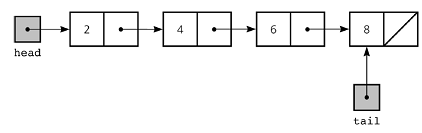
\includegraphics[width=\linewidth]{images/h3/linkedlist-in-java.png}
\caption{LinkedList}
\label{fig:core_classes}
\end{figure}
 
Gebruik een ArrayList:
\begin{itemize}
\item als je willekeurig elementen uit de lijst nodig hebt (E get(int index))
\item als je enkel element aan het einde van de lijst toevoegt en verwijdert
\end{itemize}

Gebruik een LinkedList:
\begin{itemize}
\item als je vaak doorheen alle elementen van de lijst itereert
\item als je regelmatig element vooraan of in het midden van de lijst moet toevoegen
\end{itemize}

\subsection{LinkedList als FIFO}
In het dit voorbeeld illustreren we hoe je de LinkedList kan gebruiken als een FIFO.

\begin{lstlisting}
import java.util.LinkedList;
import java.util.Queue;

public class LinkedListFIFO {

	public static void main(String[] args) {
		Queue<String> elements = new LinkedList<>();
		elements.offer("One");
		elements.offer("One");
		elements.offer("Two");
		elements.offer(null);
		elements.offer("Three");

		while (!elements.isEmpty()) {
			System.out.println(elements.remove());
		}
	}
}
\end{lstlisting}

\begin{verbatim}
One
One
Two
null
Three
\end{verbatim}


\subsection{LinkedList als LIFO}
In het volgende voorbeeld wordt de LinkedList als LIFO gebruikt.

\begin{lstlisting}
import java.util.Deque;
import java.util.LinkedList;
import java.util.Queue;

public class LinkedListLIFO {

	public static void main(String[] args) {
		Deque<String> elements = new LinkedList<>();
		elements.push("One");
		elements.push("One");
		elements.push("Two");
		elements.push(null);
		elements.push("Three");

		while (!elements.isEmpty()) {
			System.out.println(elements.pop());
		}
	}
}
\end{lstlisting}

\begin{verbatim}
Three
null
Two
One
One
\end{verbatim}

\subsection{LinkedList en ArrayDeque}

De ArrayDeque klasse is nog een alternatief voor LinkedList die minder geheugen nodig heeft.
\textit{null} kan je niet toevoegen in een ArrayDeque. ArrayDeque is verder ook 
effici\"enter als er elementen vooraan of aan het einde van de verzameling toegevoegd of verwijderd moeten worden. Als er elementen verwijderd moeten worden tijdens het doorlopen van de verzameling, dan kies je best voor LinkedList.

\begin{oefening}
We willen voor ieder kijkersprofiel in onze streaming service 2 verzamelingen bijhouden nl. ``recently watched'' en ``currently watching''. De eerste verzameling bevat de Content-objecten die we recent hebben uitgekeken. De tweede lijst bevat de Content die we momenteel kijken maar nog niet be\"eindigd hebben. 
Welke collection klasse ga je gebruiken? Voorzie in de klasse Profile de methoden \textit{startWatching(Content content)} en \textit{finishWatching(Content content)}.
Wanneer je de methode \textit{startWatching(Content content)} aanroept, voeg je de Content vooraan de verzameling ``recently watched'' toe. Zorg dat het Content-object maar 1 keer in de lijst voorkomt. De methode  \textit{finishWatching(Content content)} zorgt ervoor dat het Content-object niet langer voorkomt in de verzameling ``currently watching'' maar wel in de verzameling ``recently watched''. Test alles grondig!
\end{oefening}

\begin{figure}[H]
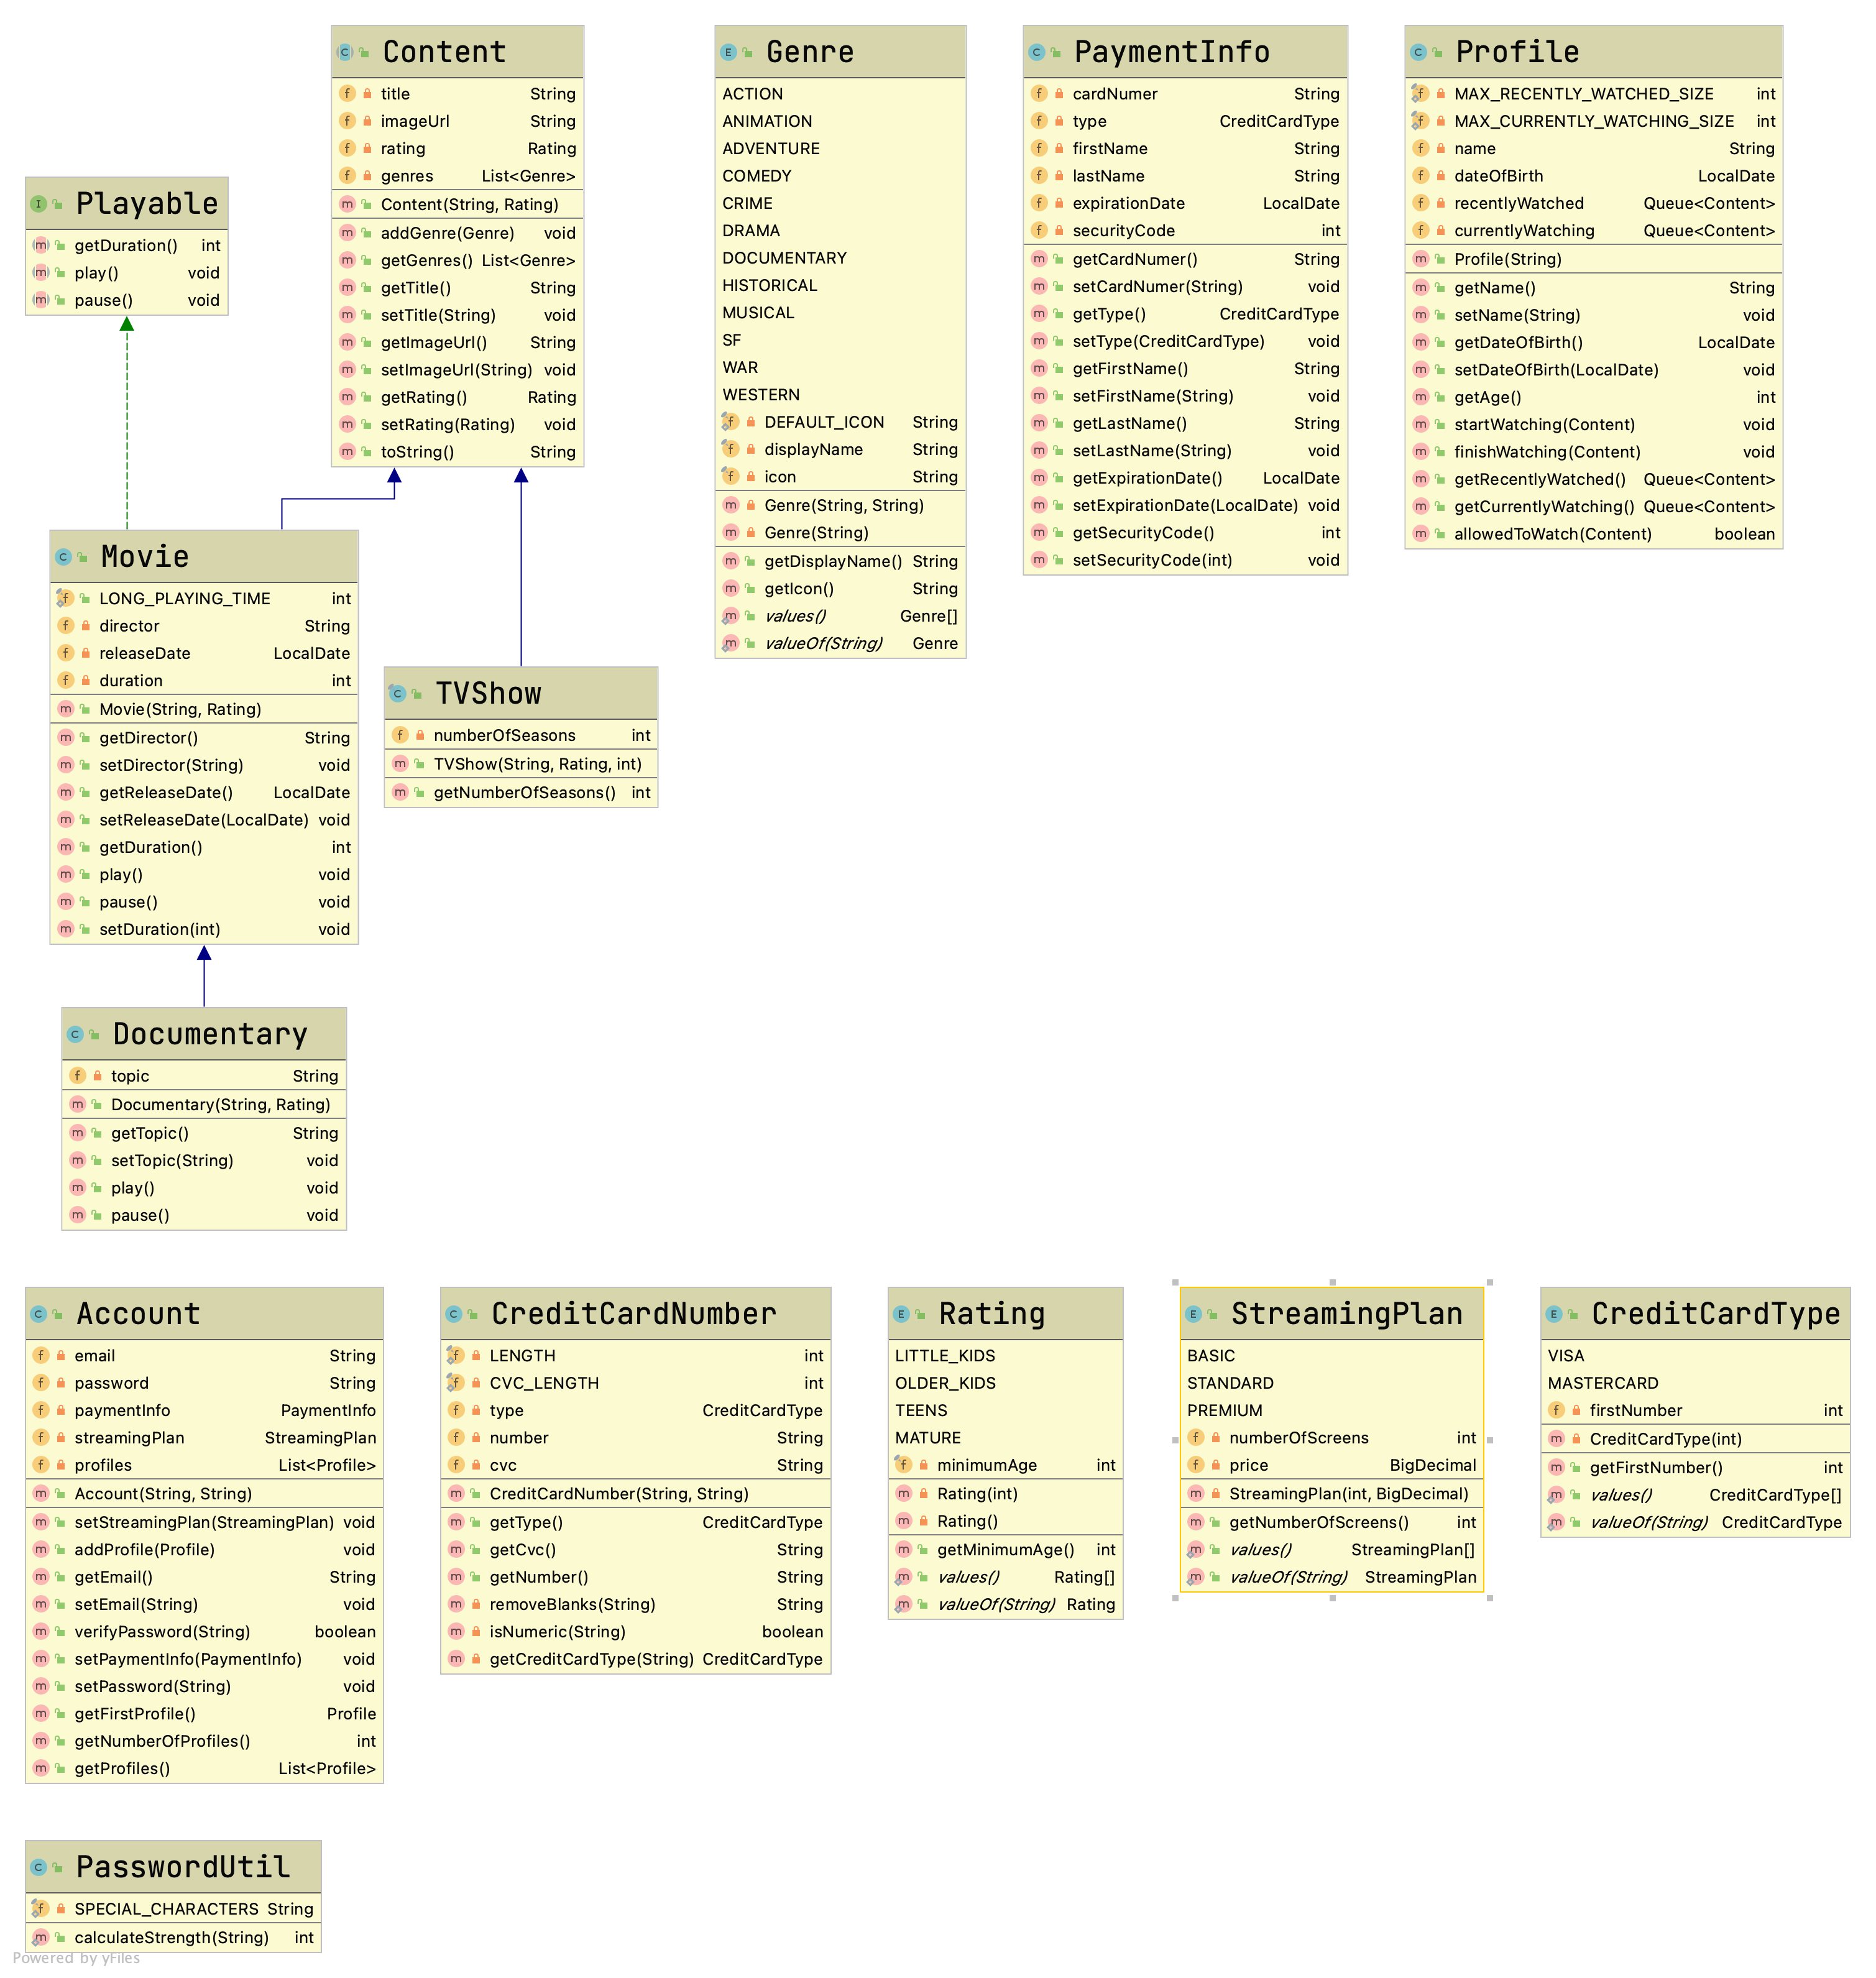
\includegraphics[width=\linewidth]{images/klassendiagram/diagram_H4.png}
\caption{Klassendiagram}
\label{fig:klassendiagram}
\end{figure}

\subsection{Performantie van ArrayList en LinkedList}

Door de uitvoer van het programma ArrayListVsLinkedList te bestuderen, krijg je een beetje inzicht in het verschil van performantie tussen ArrayList en LinkedList.
Bekijk bijvoorbeeld eens hoeveel tijd het kost om in beide verzamelingen het element op de middelste positie op te vragen en om de hele verzameling te doorlopen en alle String-objecten die starten met een 'a' te verwijderen.

\begin{lstlisting}
import java.util.ArrayList;
import java.util.Iterator;
import java.util.LinkedList;
import java.util.List;
import java.util.Random;

public class ArrayListVsLinkedList {

	private static final int ITEMS = 9999999;

	public static void main(String[] args) {
		List<String> data1 = new ArrayList<>();
		List<String> data2 = new LinkedList<>();

		for (int i = 0; i < ITEMS; i++) {
			String e = generateString(8);
			data1.add(e);
			data2.add(e);
		}

		add(data1, 0, "first");
		add(data2, 0, "first");
		add(data1, ITEMS/2, "middle");
		add(data2, ITEMS/2, "middle");
		add(data1, ITEMS, "last");
		add(data2, ITEMS, "last");

		indexOf(data1, "first");
		indexOf(data2, "first");
		indexOf(data1, "middle");
		indexOf(data2, "middle");
		indexOf(data1, "last");
		indexOf(data2, "last");

		get(data1, 0);
		get(data2, 0);
		get(data1, data1.size() / 2);
		get(data2, data2.size() / 2);
		get(data1, data1.size() - 1);
		get(data2, data2.size() - 1);

		remove(data1, "first");
		remove(data2, "first");
		remove(data1, "middle");
		remove(data2, "middle");
		remove(data1, "last");
		remove(data2, "last");

		remove(data1, 0);
		remove(data2, 0);
		remove(data1, data1.size() / 2);
		remove(data2, data2.size() / 2);
		remove(data1, data1.size() - 1);
		remove(data2, data2.size() - 1);
		
		data1 = new ArrayList<>(data1.subList(0, ITEMS / 10));
		data2 = new LinkedList<>(data2.subList(0, ITEMS / 10));
		removeAllStartingWithA(data1);
		removeAllStartingWithA(data2);
	}

	public static void remove(List<String> data, String value) {
		long start = System.currentTimeMillis();
		boolean removed = data.remove(value);
		long time = System.currentTimeMillis() - start;
		System.out.println(data.getClass().getSimpleName() + ": " + value + " removed in " + time + "ms");
	}

	public static void get(List<String> data, int index) {
		long start = System.currentTimeMillis();
		String result = data.get(index);
		long time = System.currentTimeMillis() - start;
		System.out.println(data.getClass().getSimpleName() + ": " + result + " at index " + index + " found  in " + time + "ms");
	}

	public static void remove(List<String> data, int index) {
		long start = System.currentTimeMillis();
		String remove = data.remove(index);
		long time = System.currentTimeMillis() - start;
		System.out.println(data.getClass().getSimpleName() + ": " + remove + " removed from index " + index + " in " + time + "ms");
	}

	public static void removeAllStartingWithA(List<String> data) {
		long start = System.currentTimeMillis();
		Iterator<String> iterator = data.iterator();
		while (iterator.hasNext()) {
			if (iterator.next().startsWith("a")) {
				iterator.remove();
			}
		}
		long time = System.currentTimeMillis() - start;
		System.out.println(data.getClass().getSimpleName() + ": remove starting with a in " + time + "ms");
	}

	public static void add(List<String> data, int index, String value) {
		long start = System.currentTimeMillis();
		data.add(index, value);
		long time = System.currentTimeMillis() - start;
		System.out.println(data.getClass().getSimpleName() + ": " + value + " added at  " + index + " in " + time + "ms");
	}

	public static void indexOf(List<String> data, String value) {
		long start = System.currentTimeMillis();
		int i = data.indexOf(value);
		long time = System.currentTimeMillis() - start;
		System.out.println(data.getClass().getSimpleName() + ": " + value + " found at index " + i + " in " + time + "ms");
	}


	public static String generateString(int length) {
		int leftLimit = 97; // letter 'a'
		int rightLimit = 122; // letter 'z'
		Random random = new Random();
		StringBuilder buffer = new StringBuilder(length);
		for (int i = 0; i < length; i++) {
			int randomLimitedInt = leftLimit + (int)
					(random.nextFloat() * (rightLimit - leftLimit + 1));
			buffer.append((char) randomLimitedInt);
		}
		return buffer.toString();
	}

}
\end{lstlisting}

\section{De klasse HashSet}

De HashSet is een verzameling waarin ieder element uniek is. 
Het is aan de hand van de implementatie van equals() en hashCode() van de klasse van de elementen van de HashSet dat beslist wordt of een element uniek is of niet.

\begin{lstlisting}
import java.util.HashSet;
import java.util.Set;

public class HashSetDemo {

	public static void main(String[] args) {
		Set<String> daysOfWeek = new HashSet<>();

		// Adding new elements to the HashSet
		daysOfWeek.add("Monday");
		daysOfWeek.add("Tuesday");
		daysOfWeek.add("Wednesday");
		daysOfWeek.add("Thursday");
		daysOfWeek.add("Friday");
		daysOfWeek.add("Saturday");
		daysOfWeek.add("Sunday");

		// Adding null is allowed
		daysOfWeek.add(null);

		// Adding duplicate elements will be ignored
		daysOfWeek.add("Monday");

		System.out.println(daysOfWeek);
	}

}
\end{lstlisting}


\section{De klasse PriorityQueue}

In een PriorityQueue worden alle elementen gerangschikt volgens hun natuurlijke volgorde. Voor integers is dit van klein naar groot, voor String is dit alfabetisch volgens de volgorde in de ASCII-tabel. Sorteren van objecten van eigen klassen, zonder een natuurlijke volgorde, komt aan bod in het hoofdstuk Generics.

\begin{lstlisting}
public class CreatePriorityQueueExample {
    public static void main(String[] args) {
        // Create a Priority Queue
        PriorityQueue<Integer> numbers = new PriorityQueue<>();

        // Add items to a Priority Queue (ENQUEUE)
        numbers.add(750);
        numbers.add(500);
        numbers.add(900);
        numbers.add(100);

        // Remove items from the Priority Queue (DEQUEUE)
        while (!numbers.isEmpty()) {
            System.out.println(numbers.remove());
        }

    }
}
\end{lstlisting}

\begin{lstlisting}
import java.util.PriorityQueue;

public class PriorityQueueDemo {

	public static void main(String[] args) {

		PriorityQueue<String> namePriorityQueue = new PriorityQueue<>();

		namePriorityQueue.offer("Lisa");
		namePriorityQueue.add("Robert");
		namePriorityQueue.offer("John");
		namePriorityQueue.add("Chris");
		namePriorityQueue.add("Angelina");
		namePriorityQueue.add("Joe");

		while (!namePriorityQueue.isEmpty()) {
			System.out.println(namePriorityQueue.peek());
			System.out.println(namePriorityQueue.poll());
		}

	}
}
\end{lstlisting}


\section{De klasse HashMap}

\subsection{Gebruik}

De klasse HashMap wordt gebruikt om key-value-koppels op te slaan. Bij het aanmaken van een HashMap geef je het datatype van je key en het datatype van je values op.
Zo kan je bijvoorbeeld de HashMap\textless String, Person\textgreater gebruiken om Persoon-objecten op te slaan met bijvoorbeeld hun rijksregisternummer als opzoekwaarde (key). De elementen in de HashMap zijn niet geordend, dit betekent dat de keys noch de values opgeslaan zijn in de volgorde dat je ze hebt toegevoegd.

\begin{lstlisting}
public class PhonebookDemo {

	public static void main(String[] args) {
		Map<String,String> phoneBook = new HashMap<>();
		phoneBook.put("Ben", "+32 11 77 55 10");
		phoneBook.put("Gerrit", "+32 11 77 55 16");
		phoneBook.put("Rudy", "+ 32 11 77 56 91");
		phoneBook.put("Heidi", "+32 11 77 58 01");

		System.out.println(phoneBook.get("Ben"));
		System.out.println(phoneBook.containsKey("Els"));
		System.out.println(phoneBook.values());
	}
}
\end{lstlisting}

\begin{oefening}
Breid bovenstaand programma uit en doorloop eens alle key-value-koppels in de HashMap en toon ze in de console. Wat kan je vertellen over de volgorde waarin ze worden getoond?
\end{oefening}

\subsection{Hashmap for caching}

Het duurt eventjes om de faculteit van 125000 te berekenen (er verschijnen heel wat cijfertjes op het scherm :-)). Maar vraag dit nog een tweede keer. Omdat het antwoord na de eerste berekening werd opgeslaan, verschijnt het onmiddelijk op het scherm. 

\begin{lstlisting}
import java.math.BigDecimal;
import java.util.HashMap;
import java.util.Map;
import java.util.Scanner;

public class HashmapCachingDemo {
	private Map<Integer, BigDecimal> cache = new HashMap<>();

	public static void main(String[] args) {
		HashmapCachingDemo hashmapCachingDemo = new HashmapCachingDemo();
		System.out.println("Van welk getal wil je de faculteit berekenen?");
		System.out.println("Geef 0 of een negatief getal om te stoppen.");
		Scanner scanner = new Scanner(System.in);
		int number = scanner.nextInt();
		while (number > 0) {
			BigDecimal faculty = hashmapCachingDemo.calculateFaculty(number);
			System.out.println(faculty);
			System.out.println("Van welk getal wil je de faculteit berekenen?");
			number = scanner.nextInt();
		}
	}

	public BigDecimal calculateFaculty(int number) {
		if (cache.containsKey(number)) {
			return cache.get(number);
		}
		BigDecimal result = BigDecimal.ONE;
		BigDecimal multiplier = BigDecimal.valueOf(2);
		while (multiplier.compareTo(BigDecimal.valueOf(number)) <= 0) {
			result = result.multiply(multiplier);
			multiplier = multiplier.add(BigDecimal.ONE);
		}
		cache.put(number, result);
		return result;
	}
}
\end{lstlisting}

\begin{oefening}
Voorzie de klasse Book.  In de klasse Book voorzien we 3 eigenschappen: naam, beschrijving en jaar van publicatie. Voorzie een constructor met 3 parameters, getters en setters en een toString() methode. De output van de toString mag je zelf kiezen.

Maak nu een interface Library met de volgende methoden: addBook en getBookByName.  Je voorziet 2 implementaties LibraryWithHashMap en LibraryWithArrayList. In de implementatie LibraryWithHashMap maak je gebruik van een HashMap om de boeken op te slaan. De naam van het boek gebruik je als key in de HashMap, het Book-object is de value. Implementeer beide methoden uit de interface. In de andere klasse, LibraryWithArrayList gebruik je een ArrayList om de toegevoegde boeken bij te houden. 
Maak nu een hoofdprogramma waarin je een aantal random gegenereerde boeken in zowel een instantie van de LibraryWithHashMap als LibraryWithArrayList toevoegt.  Zorg dat je ook 1 boek toevoegt waarvan je de naam kent. Hoe lang duurt het om dit boek op te vragen met behulp van de methode getBookByName? Voer je programma enkele keren uit met telkens een verschillend aantal random gegenereerde boeken.
\end{oefening}

\begin{remark}
  Meer weten over collections in java, kijk op pluralsight: \url{https://app.pluralsight.com/library/courses/java-collections-fundamentals}.
  Het onderwerp Java Streams komt later in de cursus aan bod.
\end{remark}

\chapter{Generics}

\begin{summary}
Generics biedt de mogelijkheid om generieke code te schrijven die onafhankelijk is van een datatype. Op het moment dat een ontwikkelaar een generieke klasse, interface of methode gaat gebruiken, zal hij aangeven welk datatype hij wenst te gebruiken. Je hebt generics al toegepast in het vorige hoofdstuk. Het Java Collections framework is volledig generiek geschreven. Op het ogenblik dat je een ArrayList gebruikt, geef je aan welk datatype de elementen van jouw ArrayList zullen hebben.
\end{summary}

\section{V\'o\'or generics}
Java is een streng getypeerde programmeertaal. Tijdens het compileren van een programma, zal je er al op gewezen worden als je een verkeerd datatype gebruikt.

\begin{lstlisting}
Content aReference = new Movie("Brother Bear", Rating.LITTLE_KIDS);
Integer luckyNumber = aReference;
\end{lstlisting}

De tweede lijn code geeft een compileerfout. 

Toen Java werd ge\"introduceerd, was deze controle niet aanwezig in het Java Collections framework. 

De volgende code zal geen enkel probleem opleveren tijdens het compileren.

\begin{lstlisting}
import java.util.ArrayList;
import java.util.Iterator;

public class BeforeGenerics {

	public static void main(String[] args) {
		ArrayList objecten = new ArrayList();
		objecten.add(1);
		objecten.add(5.4);
		objecten.add(new Movie("Inception", Rating.MATURE));

		Iterator iterator = objecten.iterator();
		double total = 0;
		while (iterator.hasNext()) {
			total += (Double) iterator.next();
		}
		System.out.println(total);
	}
}
\end{lstlisting}

Het loopt echter mis zodra je de code gaat uitvoeren.

\begin{verbatim}
Exception in thread "main" java.lang.ClassCastException: class java.lang.Integer 
cannot be cast to class java.lang.Double (java.lang.Integer and java.lang.Double 
are in module java.base of loader 'bootstrap')
	at be.pxl.ja.BeforeGenerics.main(BeforeGenerics.java:24)
\end{verbatim}

V\'o\'or Java 5 was er dus geen type-safety wanneer je klassen uit het Java Collections framework gebruikte. Sinds Java 5 is dit gelukkig veranderd.
Wanneer je de huidige implementatie van de klasse java.util.ArrayList er even bijneemt, ontdekt je hier een parameter  $<E>$. 
Deze E is de type-parameter en laat je toe om de ArrayList te typeren. Je kan dus duidelijk maken van welk datatype je objecten toelaat in je ArrayList.

\begin{lstlisting}
/**
 * Resizable-array implementation of the {@code List} interface.  Implements
 * all optional list operations, and permits all elements, including
 * {@code null}. 
 * ...
 * @param <E> the type of elements in this list
 *
 * @author  Josh Bloch
 * @author  Neal Gafter
 * @see     Collection
 * @see     List
 * @see     LinkedList
 * @see     Vector
 * @since   1.2
 */
public class ArrayList<E> extends AbstractList<E>
        implements List<E>, RandomAccess, Cloneable, java.io.Serializable {
        
    transient Object[] elementData;
    
    /**
     * Returns the element at the specified position in this list.
     *
     * @param  index index of the element to return
     * @return the element at the specified position in this list
     * @throws IndexOutOfBoundsException {@inheritDoc}
     */
    public E get(int index) {
        Objects.checkIndex(index, size);
        return elementData(index);
    }
    
    E elementData(int index) {
        return (E) elementData[index];
    }
    
    ...
}
\end{lstlisting}

\begin{lstlisting}
import java.util.ArrayList;
import java.util.Iterator;

public class SinceGenerics {

	public static void main(String[] args) {

		ArrayList<Double> objecten = new ArrayList<>();
		objecten.add((double) 1);
		objecten.add(5.4);
		//objecten.add(new Movie("Inception", Rating.MATURE));

		Iterator<Double> iterator = objecten.iterator();
		double total = 0;
		while (iterator.hasNext()) {
			total += iterator.next();
		}
		System.out.println(total);
	}
}
\end{lstlisting}

Bij het aanroepen van de constructor van een generieke klasse gebruiken we de diamond-operator $<>$.
De compiler kan namelijk het datatype van de objecten in onze ArrayList afleiden (dit noemen we type inference). Daarom hoeven we datatype niet te herhalen bij het aanroepen van de constructor en kunnen we hier de diamond-operator gebruiken.

Wanneer je toch een Movie-object zou toevoegen aan een ArrayList die enkel Double-ojecten toelaat, krijg je een compileerfout.
\begin{verbatim}
Error:(16, 30) java: incompatible types: be.pxl.ja.streamingservice.model.Movie 
cannot be converted to java.lang.Double
\end{verbatim}

\section{Zelf generieke klassen schrijven}

De klasse Duo bevat een koppel objecten van het generieke datatype T. Dat het om een generieke klasse gaat heb je in de definitie van de klasse al aangegeven door de type-parameter T te gebruiken ($<T>$). In de klasse Duo mag je nu T gebruiken als datatype.

\begin{lstlisting}
public class Duo<T> {
	private T first;
	private T second;

	public Duo(T first, T second) {
		this.first = first;
		this.second = second;
	}

	public T getFirst() {
		return first;
	}

	public T getSecond() {
		return second;
	}
}
\end{lstlisting}

Op het ogenblik dat je objecten van de klasse Duo gaat maken, ga je aangeven door welk echte datatype de type-parameter T vervangen moet worden. Voor de ontwikkelaar lijkt het er dan op dat in de klasse de type-parameter T vervangen wordt door het gekozen datatype.


\begin{lstlisting}
public class DifferentDuos {

	public static void main(String[] args) {
		Duo<String> cocktail = new Duo<>("gin", "tonic");
		System.out.println(cocktail.getFirst());
		Duo<Actor> famousDuo = new Duo<>(new Actor("Ben","Stiller"), new Actor("Owen", "Wilson"));
		Duo<Integer> numbers = new Duo<>(5, 12);
	}

}
\end{lstlisting}

\subsection{Naamgeving}

Om verwarring te vermijden tussen echte klassen en generieke  type-parameters in Java is het belangrijk dat je de correcte naamgeving gebruikt. Zo zullen we altijd \'e\'en enkele hoofdletter gebruiken om een type-parameter te benoemen.
Volgens de code conventies mag je een enkele hoofdletter nooit gebruiken als naam voor een klasse, je moet altijd zinvolle klassenamen gebruiken.
Wanneer je dus een enkele hoofdletter ziet staan in Java code, mag je ervan uitgaan dat het om een generieke parameter gaat. 

Verder houden we ons nog aan de volgende richtlijnen:

\begin{itemize}
\item E – Element (gebruikt in het Java Collections Framework)
\item K – Key (gebruikt in Map)
\item N – Number
\item T – Type
\item V – Value (gebruikt in Map)
\item S,U,V etc. – Type te gebruiken indien T reeds in gebruik is
\end{itemize}

\section{Generieke interfaces}

\subsection{Interface $Comparable<T>$}

De generieke interface $Comparable<T>$ maakt het mogelijk om de objecten, van een klasse die de $Comparable<T>$ interface implementeert, te rangschikken. We zeggen dan dat die klasse een natuurlijke volgorde heeft.
Zodra een klasse deze interface implementeert, kan je bijvoorbeeld de methode Collections.sort(...) gebruiken om een Collection met objecten van deze klasse te sorteren. 

Als een klasse de interface $Comparable<T>$ implementeert, dan vul je de type-parameter T in met de klasse zelf. Je bent dan verplicht om de methode \textit{int compareTo(T e)}  te implementeren. Door de implementatie van deze methode kan je ieder object van de klasse vergelijken met een ander object van dezelfde klasse. 
De methode \textit{int compareTo(T e)} geeft volgende return-waarde:
\begin{itemize}
\item 0 indien beide objecten gelijk zijn.
\item -1 of een negatief getal als \textit{this} kleiner is dan het argument.
\item 1 of een positief getal indien \textit{this} groter is dan het argument.
\end{itemize}

Probeer steeds de natuurlijke volgorde van een klasse consistent te houden met de implementatie van equals. Dus wanneer e1.compareTo(e2) == 0 dan geeft ook e1.equals(e2) en e2.equals(e1) true. Null behoort tot geen enkele klasse, dus e1.compareTo(null) moet steeds een NullPointerException opgooien.


\begin{figure}[H]
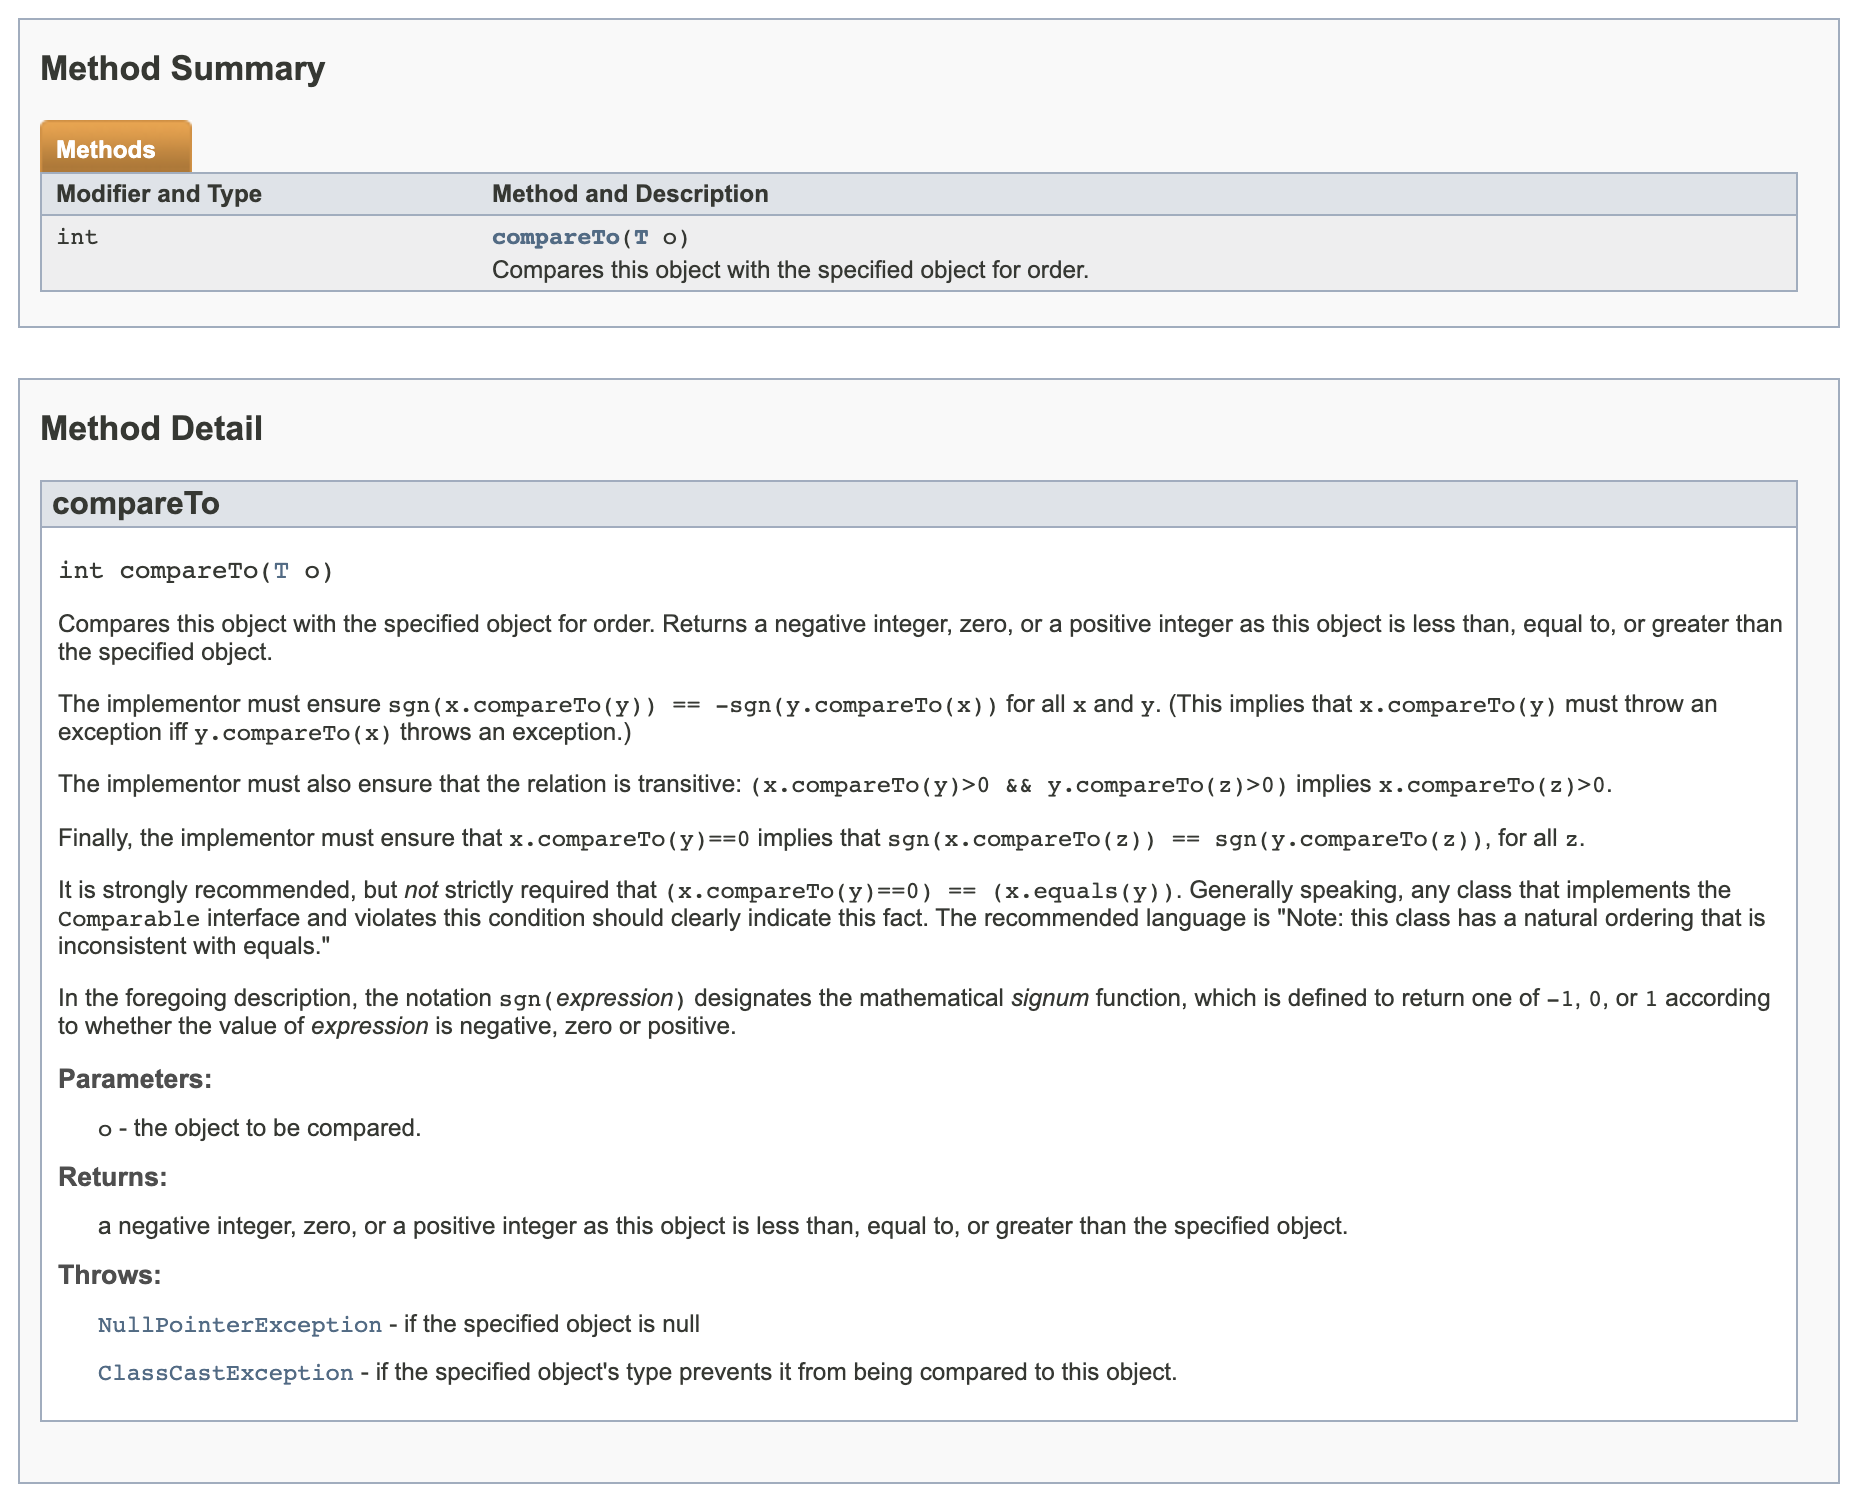
\includegraphics[width=\linewidth]{images/h4/javadoc_compareTo.png}
\caption{Java documentatie voor $Comparable<T>$}
\label{fig:core_classes}
\end{figure}

De klasse Profile krijgt een natuurlijke volgorde op basis van de naam (name) van het profiel. Profile-objecten kunnen dus steeds alfabetisch op naam gerangschikt worden.

\begin{lstlisting}
public class Profile implements Comparable<Profile> {
	private String name;
	private LocalDate dateOfBirth;

	public Profile(String name) {
		this.name = name;
	}
	
	public void setDateOfBirth(LocalDate dateOfBirth) {
		if (dateOfBirth.isAfter(LocalDate.now())) {
			throw new InvalidDateException(dateOfBirth, "date of birth", "No date of birth in future allowed.");
		}
		this.dateOfBirth = dateOfBirth;
	}
	
	public int getAge() {
		if (dateOfBirth == null) {
			return 0;
		}
		return (int) ChronoUnit.YEARS.between(dateOfBirth, LocalDateTime.now());
	}
	
	@Override
	public int compareTo(Profile other) {
		return this.name.compareTo(other.name);
	}
	
	@Override
	public boolean equals(Object o) {
		if (this == o) {
			return true;
		}
		if (o == null || getClass() != o.getClass()) {
			return false;
		}

		Profile profile = (Profile) o;

		return getName() != null ? getName().equals(profile.getName()) : profile.getName() == null;
	}

	@Override
	public String toString() {
		return "Profile{" +
				"name='" + name + '\'' +
				'}';
	}
}
\end{lstlisting}

\begin{lstlisting}
import java.util.ArrayList;
import java.util.Collections;
import java.util.List;

public class AlphabeticSortingProfiles {

	public static void main(String[] args) {
		List<Profile> profiles = new ArrayList<>();
		Profile profile1 = new Profile("Erik");
		Profile profile2 = new Profile("Sam");
		Profile profile3 = new Profile("Ann");
		Profile profile4 = new Profile("Ann");

		profiles.add(profile1);
		profiles.add(profile2);
		profiles.add(profile3);
		profiles.add(profile4);

		System.out.println(profile3.compareTo(profile4));
		System.out.println(profile4.compareTo(profile2));

		Collections.sort(profiles);
		
		System.out.println(profiles);
	}
}
\end{lstlisting}

Je zou er ook voor kunnen kiezen dat de natuurlijke sortering van Profile-objecten op leeftijd gebaseerd is, bijvoorbeeld van jong naar oud. In dat geval kan je de compareTo() methode als volgt implementeren.

\begin{lstlisting}
@Override
public int compareTo(Profile other) {
	return getAge() - other.getAge();
}
\end{lstlisting}

\subsection{Eigen generieke interface}

Naast generieke klassen kan je ook generieke interfaces en methoden ontwikkelen.
Hier is een voorbeeld van een generieke interface met 2 type-parameters T en U.

\begin{lstlisting}
public interface Service<T,U> {

	T execute(U arg);
}
\end{lstlisting}

Als je beslist om deze interface te implementeren ben je verplicht om de methode execute te implementeren, maar je ben vrij om het datatype voor de parameter en de return-waarde te kiezen.

Hier volgen 2 klassen die de interface Service implementeren.

\begin{lstlisting}
public class CountService implements Service<Integer, String> {

	@Override
	public Integer execute(String arg) {
		return arg.length();
	}
}
\end{lstlisting}

\begin{lstlisting}
import java.util.Random;

public class ProfileService implements Service<Profile, Integer> {

	private static final Random RANDOM = new Random();

  /**
	 * This method can be used to create a Profile-object with a random name and age 18.
	 *
	 * @param length length of the random name of the newly created Profile
	 * @return a newly created Profile-object with a random name of given length and age 18.
	 */
	public Profile execute(Integer length) {
		StringBuilder builder = new StringBuilder();
		for (int i = 0; i < length; i++) {
			int number = RANDOM.nextInt(26) + 97;
			builder.append((char) number);
		}
		Profile profile = new Profile(builder.toString());
		profile.setDateOfBirth(LocalDate.now().minusYears(18));
		return profile;
	}
}
\end{lstlisting}


\begin{lstlisting}
public class GenericServiceDemo {

	public static void main(String[] args) {

		CountService countService = new CountService();
		System.out.println(countService.execute("abcdefghijkl"));

		ProfileService profileService = new ProfileService();
		Profile profile1 = profileService.execute(8);
		System.out.println(profile1);
	}
}
\end{lstlisting}

De uitvoer van bovenstaand programma kan volgende output geven.
\begin{verbatim}
12
Profile{name='tsxjpsol',age=18}
\end{verbatim}


\section{Generieke functies}

Indien je geen nood hebt aan een volledige geparametrizeerde klasse, is het ook mogelijk om geparametrizeerde functies te maken. Zowel gewone als static functies kunnen \'e\'en of meerdere generieke types bevatten. Zelfs een constructor kan gebruikmaken van  generieke types.

Hier volgt een voorbeeld. 
Onderstaande static functie occursExactTimes geeft true indien het opgegeven item het exact opgegeven aantal keren voorkomt in de List. Indien dat niet het geval is, wordt false gegeven.
V\'o\'or het returntype van de functie plaats je eerst een opsomming van de generieke types die gebruikt worden. 
 
\begin{lstlisting}
import java.util.List;

public class OccurenceUtil {

	public static <T> boolean occursExactTimes(List<T> items, T item, int times) {
		int count = 0;
		for (T anItem : items) {
			if (anItem.equals(item)) {
				count++;
			}
		}
		return count == times;
	}

}
\end{lstlisting}

De functie occursExactTimes kan nu gebruikt worden voor elk gewenst datatype.

\begin{lstlisting}
import java.util.Arrays;
import java.util.List;

public class OccurenceUtilDemo {

	public static void main(String[] args) {
		
		List<Integer> numbers = Arrays.asList(7,15,23,12,8,7,23,13,32,7);
		System.out.println(OccurenceUtil.occursExactTimes(numbers, 7, 3));
		System.out.println(OccurenceUtil.occursExactTimes(numbers, 23, 5));

		List<Profile> profiles = Arrays.asList(
				new Profile("Ann"),
				new Profile("Mary"),
				new Profile("Henk"),
				new Profile("Thomas"),
				new Profile("Ann"));
		System.out.println(OccurenceUtil.occursExactTimes(profiles, new Profile("Ann"), 3));
		System.out.println(OccurenceUtil.occursExactTimes(profiles, new Profile("Tommy"), 0));
	}
}
\end{lstlisting}

Bestudeer de code. Welke uitvoer verwacht je?
Komt dat overeen met onze uitvoer? 

\begin{verbatim}
true
false
false
true
\end{verbatim}

\section{Wildcards en bounds}

\subsection{Bounded wildcards}

Bestudeer het volgende programma.

\begin{lstlisting}
import java.util.ArrayList;
import java.util.List;

public class WildcardDemo {


	public static void main(String[] args) {
		List<Movie> movies = new ArrayList<>();
		Movie brotherBear = new Movie("Brother Bear", Rating.LITTLE_KIDS);
		brotherBear.setDuration(125);
		Movie theLionKing = new Movie("The Lion King", Rating.LITTLE_KIDS);
		brotherBear.setDuration(135);
		movies.add(brotherBear);
		movies.add(theLionKing);
		System.out.println(totalDuration(movies));

		List<Documentary> documentaries = new ArrayList<>();
		Documentary planetEarth = new Documentary("Planet Earth", Rating.OLDER_KIDS);
		planetEarth.setDuration(200);
		Documentary ourOcean = new Documentary("Our Ocean", Rating.OLDER_KIDS);
		planetEarth.setDuration(140);
		
		System.out.println(totalDuration(documentaries));
	}


	public static int totalDuration(List<Movie> movies) {
		int totalDuration = 0;
		for (Movie movie: movies) {
			totalDuration += movie.getDuration();
		}
		return totalDuration;
	}
}
\end{lstlisting}

De methode totalDuration kan enkel aangeroepen worden met een List met Movie-objecten. Als je een List met Documentary-objecten hebt zoals in het voorbeeld, zal je een compileerfout krijgen. Eigenlijk is dat zonde. Zou het niet gemakkelijk zijn als de methode totalDuration ook zou werken voor een List met objecten van eender welke subklasse van Movie.

We vervangen nu de signatuur:
\begin{lstlisting}
public static int totalDuration(List<Movie> movies) { ... }
\end{lstlisting}

door: 

\begin{lstlisting}
public static int totalDuration(List<? extends Movie> movies) { ... }
\end{lstlisting}

In deze nieuwe signatuur van de methode totalDuration is een klein maar belangrijk verschil. We hebben het datatype \textit{List$<$Movie$>$} vervangen door \textit{List$<$? extends Movie$>$}. Nu accepteert de methode totalDuration een lijst van eender welke subklasse van Movie, dus kunnen we het ook gebruiken voor $List<Documentary>$. 

We maken hier gebruik van het concept ``bounded wildcard''. Het ? staat voor een nog onbekend datatype, maar we leggen wel grenzen op aan dit onbekende datatype. Zo verplichten we dat dit onbekend datatype de klasse Movie of een subklasse van Movie moet zijn.

In dit voorbeeld had je ook een generieke parameter kunnen gebruiken in plaats van de wildcard, dus \textit{List$<$E extends Movie$>$}.

Je zal af en toe zien dat als  je \'e\'en type parameter gebruikt, je deze kan vervangen door een wildcard. Toch is dat niet altijd waar, kijk maar naar onderstaand voorbeeld waar secondFunction een compileerfout zal geven.
Eigenlijk mag je als vuistregel nemen dat je gegevens met een onbekend datatype (wildcard dus) mag lezen, maar niet mag schrijven.

\begin{lstlisting}
public class Experiment {
    public static <E> void firstFunction(List<E> list) {
        list.add(list.get(0));
    }

    public static void secondFunction(List<?> list) {
        list.add(list.get(0)); // !!!!!!!!!!!!!! won't compile !!!!!!!!!
    }
}
\end{lstlisting}

Er zijn nog enkele verschillen tussen wildcards en type parameters.
Bij type parameters kan je meerdere beperkingen opleggen, bij wildcards niet.

\subsection{Bounds}

Een ``bound'' of grens is een beperking die we opleggen voor de generieke type-parameter. 
Zo zal de methode \textit{void startPlayableContent(T playableContent)} enkel argumenten aanvaarden waarvoor de volgende begrezing geldig is \textit{$<$T extends Content \& Playable$>$}. Dit betekent dat we enkel de klasse Content en zijn subklassen toelaten en ook nog verwachten dat de interface Playable wordt ge\"implementeerd. 
In een begrenzing mag je maximaal 1 klasse opnemen, wat betreft het aantal interfaces is er geen restrictie. De klasse moet wel in de opsomming altijd als eerste staan:
\textit{
$<$T extends MyClass \& MyFirstInterface \& MySecondInterface \& MyThirdInterface$>$}.

\begin{lstlisting}
public class MultipleBoundsDemo {

	public static void main(String[] args) {
		List<Movie> movies = new ArrayList<>();
		Movie brotherBear = new Movie("Brother Bear", Rating.LITTLE_KIDS);
		brotherBear.setDuration(125);
		Movie theLionKing = new Movie("The Lion King", Rating.LITTLE_KIDS);
		brotherBear.setDuration(135);

		List<Documentary> documentaries = new ArrayList<>();
		Documentary planetEarth = new Documentary("Planet Earht", Rating.OLDER_KIDS);
		planetEarth.setDuration(200);
		Documentary ourOcean = new Documentary("Our Ocean", Rating.OLDER_KIDS);
		planetEarth.setDuration(140);

		startPlayableContent(ourOcean);
		startPlayableContent(brotherBear);
	}

	public static <T extends Content & Playable> void startPlayableContent(T playableContent) {
		playableContent.play();
		System.out.println("This content will be playing for " + playableContent.getDuration() + " minutes.");
	}
}
\end{lstlisting}

\subsection{Upper bound, lower bound en unbounded wildcard}

Wanneer je gebruikmaakt van wildcards is het mogelijk om upper bounds (bovengrens) en lower bounds (ondergrens) beperkingen op te leggen. Bij type parameters zijn enkel upper bounds beperkingen mogelijk.

\begin{lstlisting}
import java.util.ArrayList;
import java.util.List;

public class BoundsDemo {

	//Upper bound wildcard
	public static void deleteMovie(List<? extends Movie> movieList, Movie movie) {
		movieList.remove(movie);
	}

	//Lower bound wildcard
	public static void addDocumentary(List<? super Movie> movieList) {
		movieList.add(new Documentary("Hunt for Red October", Rating.OLDER_KIDS));
	}

	//Unbounded wildcard
	public static void printAll(List<?> list) {
		System.out.println("Number of items: " + list.size());
		for (Object item : list) {
			System.out.println(item);
		}
		System.out.println("+++++++++++++++++++++++++++++++");
	}

	public static void main(String[] args) {

		List<Content> contentList = new ArrayList<>();
		List<Movie> movieList = new ArrayList<>();
		List<Documentary> documentaryList = new ArrayList<>();

		addDocumentary(contentList);
		addDocumentary(movieList);
		//addDocumentary(documentaryList);

		printAll(contentList);
		printAll(movieList);

		Movie movie = movieList.get(0);
		deleteMovie(movieList, movie);
		printAll(movieList);
	}

}
\end{lstlisting}

De methode addDocumentary kan gebruikt worden voor $List<Movie>$ maar ook voor iedere superklasse van Movie zoals $List<Content>$ en $List<Object>$.

De methode deleteMovie kan gebruikt worden voor $List<Movie>$ maar ook voor iedere subklasse van Movie zoals $List<Documentary>$.

\begin{oefening}
In het package be.pxl.ja.oefening1 heb je de volgende klassen ter beschikking.

\begin{figure}[H]
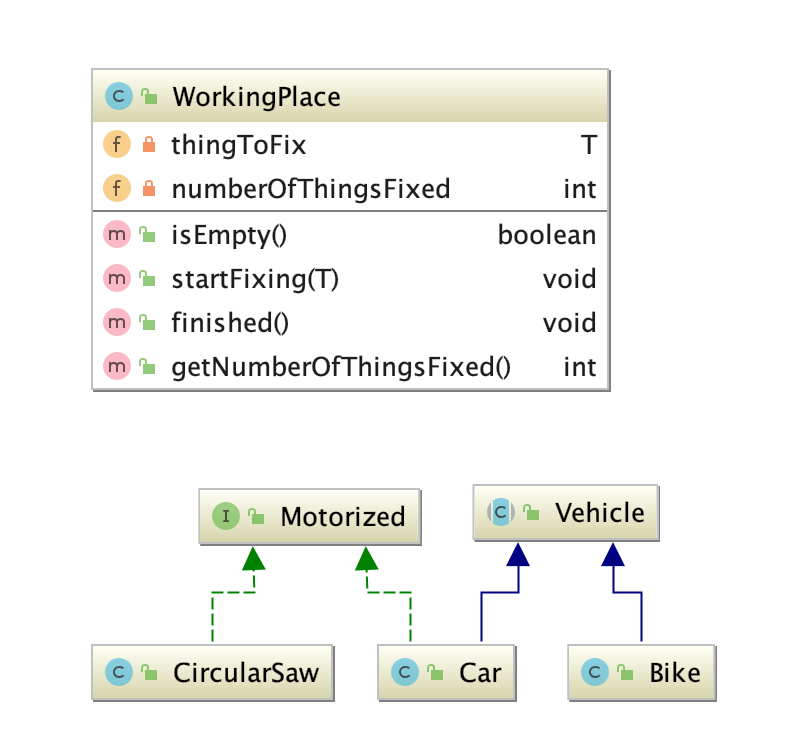
\includegraphics{images/h4/bounds_exercise_diagram.png}
\caption{Klassenhi\"erarchie}
\label{fig:bounds_exercise}
\end{figure}

\begin{enumerate}[label=(\alph*)]
\item Pas de generieke klasse WorkingPlace aan zodat je WorkingPlace-objecten kan maken om Motorized objecten te herstellen (dus wel WorkingPlace$<$Motorized$>$, WorkingPlace$<$Car$>$, WorkingPlace$<$CircularSaw$>$ maar niet WorkingPlace$<$Bike$>$ of WorkingPlace$<$Vehicle$>$)
\item Pas de generieke klasse WorkingPlace aan zodat je WorkingPlace-objecten kan maken om
Vehicle-objecten te herstellen (dus wel WorkingPlace$<$Car$>$ en WorkingPlace$<$Vehicle$>$).
\item Pas de generieke klasse WorkingPlace aan zodat je WorkingPlace-objecten kan maken om
Motorized-Vehicle-objecten te herstellen.
\end{enumerate}
We passen nu de grenzen van de parameter in de methode getScore in de WorkingPlaceUtility
klasse aan. Test dit telkens uit!
\begin{enumerate}[label=(\alph*)]
\item Zorg ervoor dat je de methode getScore uit WorkingPlaceUtility enkel kan oproepen voor
WorkingPlace$<$Bike$>$-objecten.
\item Zorg ervoor de je de methode getScore uit WorkingPlaceUtility enkel kan oproepen voor
WorkingPlace objecten die Vehicle objecten herstellen.
\item Zorg ervoor de je de methode getScore uit WorkingPlaceUtility enkel kan oproepen voor
WorkingPlace objecten die Motorized objecten herstellen.
\item  Zorg ervoor de je de methode getScore uit WorkingPlaceUtility enkel kan oproepen voor WorkingPlace objecten die Motorized Vehicle objecten herstellen. 
\end{enumerate}
\end{oefening}


\section{Erasure en problemen}

Generics bestaat enkel ``at compiletime''. 
Tijdens het compileren van Java code worden er verschillende extra controles uitgevoerd bij generieke klassen om het correcte gebruik van datatypes te garanderen. 
Vervolgens wordt bij het genereren van de bytecode alle informatie over het generieke datatype gewoon verwijderd. Dus List$<$T$>$ wordt, na enkele controles en toevoegingen van extra code door de compiler, vervangen door List$<$Object$>$ en List$<$T extends Movie$>$ wordt List$<$Movie$>$. Dit noemen we \textbf{type erasure}. In Java zal er dus ook altijd maar \'e\'en gecompileerde klasse (.class-bestand) gegenereerd worden voor een generieke klasse. 

\begin{lstlisting}
List<Integer> list1 = new ArrayList<>();
List<Float> list2 = new ArrayList<>();
if (list1.getClass() == list2.getClass()) {
	System.out.println("Lists have same class.");
}
\end{lstlisting}

Door type erasure is het dus niet mogelijk om generieke static eigenschappen in een klasse te maken.
Ook is het niet mogelijk om een constructor van een generiek datatype aan te roepen.
Daarnaast is het ook niet mogelijk om het generiek datatype te gebruiken bij de operator instanceof.

\begin{lstlisting}
class Box<T> {
   //compiler error
   private static T value;
   private T t;
   
   public Box() {
      // compiler error
   	  t = new T();
   }

   public void set(T t) {
      this.t = t;
   }

   public T get() {
      return t;
   } 
   
   public boolean test() {
	  return t instanceof T;
   }  
}
\end{lstlisting}

\begin{remark}
  Meer weten over generics in java, kijk op pluralsight: \url{https://app.pluralsight.com/player?course=java-generics}. We hebben niet alle onderwerpen die in deze pluralsight cursus aan bod komen gezien.
\end{remark}


\section{Oefening}

\begin{oefening}
Maak een abstract klasse Player met een member variabele name. Voorzie een constructor met name als parameter. 
\\

Maak van deze abstract klasse Player 3 afgeleide klassen: BaseballPlayer, VolleybalPlayer en SoccerPlayer.
\\

Maak nu een klasse Team met de volgende eigenschappen: 
\begin{itemize}
\item name
\item played (=aantal wedstrijden gespeeld)
\item won (= aantal wedstrijden gewonnen)
\item lost (= aantal wedstrijden verloren)
\item tied (=aantal wedstrijden gelijkgespeeld) 
\item members (verzameling van spelers)
\end{itemize}
Voorzie enkel getters. In de constructor geef je  een naam mee voor het team.
\\

Voorzie de methode addPlayer om een speler aan het team toe voegen en een methode
numberOfPlayers om te vragen hoeveel spelers er in het team zitten.
\\

\textbf{Kan je spelers met een verschillend type (bv. BaseballPlayer en SoccerPlayer) in één team
toevoegen? Test uit! Zorg ervoor dat dit niet (meer) mogelijk is.}
\\

Voorzie de methode matchResult(Team opponent, int ourScore, int theirScore). Deze methode zorgt ervoor dat voor het Team waarvoor de methode wordt aangeroepen en de opponent het aantal gespeelde, gewonnen, verloren en gelijkspel wedstrijden wordt opgehoogd afhankelijk van de waarden van ourScore en theirScore.
\\

\textbf{Kan je bovenstaande methode aanroepen voor een team van volleybalspelers tegen een team van baseballspelers? Los dit eventueel op, zodat dat niet langer mogelijk is.}
\\

Voeg tenslotte een methode ranking() toe. Deze geeft een geheel getal terug waarbij het team 3 punten krijgt voor elke gewonnen wedstrijd en 1 punt voor gelijkspel.
Zorg nu dat je een verzameling met Team-objecten kunt aanmaken en deze kunt sorteren op basis van de ranking.
\end{oefening}

\chapter{Geneste klassen en lambda expressies}

\section{Geneste klassen}

In Java is het mogelijk om een klasse te defini\"eren binnen een bestaande klasse. Dit noemen we een geneste klasse of \textit{nested class}. Er zijn 2 categorie\"en van geneste klassen: static en non-static.
De geneste klassen die als static worden gedefinieerd noemen we eenvoudigweg \textit{static nested classes}. Non-static nested classes worden ook \textit{inner classes} genoemd. In de praktijk zal je zien dat de termen \textit{nested} en \textit{inner} vaak door elkaar worden gebruikt.

\begin{figure}[H]
  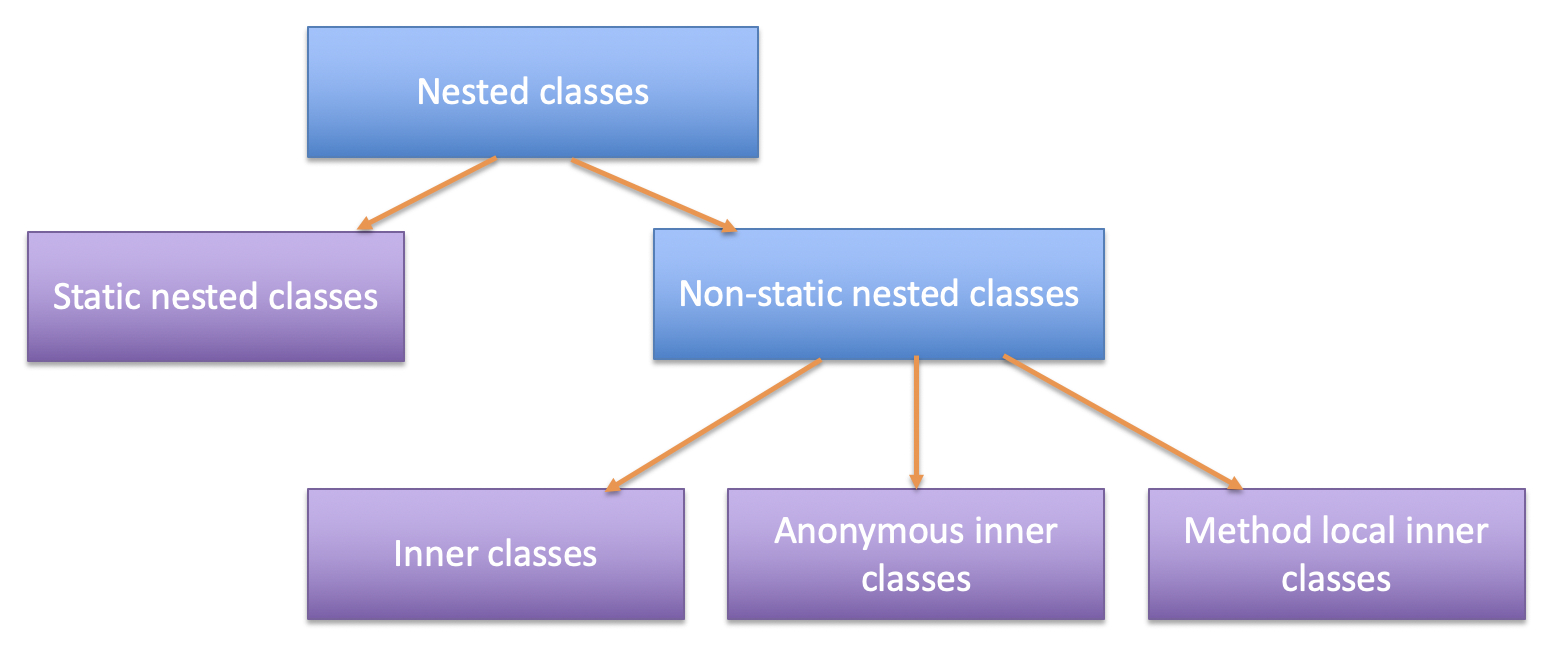
\includegraphics[width=\linewidth]{images/h5/nested-classes.png}
  \caption{Soorten geneste klassen}
  \label{fig:nested_classes}
\end{figure}

We illustreren elke type van de geneste klassen met een voorbeeld.


\subsection{Inner classes}

\begin{lstlisting}
import java.util.ArrayList;
import java.util.List;

public class CPU {

	private List<Core> cores;
	private String manufacturer;

	public CPU(int numberOfCores, double clockspeed, String manufacturer) {
		cores = new ArrayList<>();
		for (int i = 0; i < numberOfCores; i++) {
			cores.add(new Core(clockspeed));
		}
		this.manufacturer = manufacturer;
	}

	public int getNumberOfCores() {
		return cores.size();
	}

	public class Core {
		private double clockspeed;

		public Core(double clockspeed) {
			this.clockspeed = clockspeed;
		}

		public double getClockspeed() {
			return clockspeed;
		}

		public String getManufacturer() {
			return manufacturer;
		}
	}

	public static void main(String[] args) {
		CPU cpu = new CPU(4, 3.0, "AMD");
		System.out.println(cpu.getNumberOfCores());

		Core newCore = cpu.new Core(4.0);
		System.out.println(newCore.getManufacturer());
	}

}
\end{lstlisting}

Onze \textit{inner class} Core heeft toegang tot de eigenschappen van de \textit{outer class} CPU. Je moet ook eerst een object van de \textit{outer class} aanmaken om een object van de \textit{inner class} te kunnen maken.

\begin{oefening}
Maak een klasse \textit{Car} met een inner class \textit{Engine}.
Voeg in beide klassen een methode \textit{void start()} toe.
De klasse Car heeft 2 eigenschappen: engine en fuel (String). 
In de constructor van de klasse Car maak je het Engine-object aan, de waarde voor eigenschap fuel krijg je mee als parameter.
Wanneer voor een Car-object de methode start() wordt aangeroepen, roep je de methode start() van de engine aan. De methode start() in de klasse engine drukt een tekstfragment af met vermelding dat de motor is gestart en het soort brandstof (fuel) dat door de motor wordt verbruikt.

Maak een programma waarin je een object maakt van de klasse Car. Roep de method start() aan. Kan je ook een object aanmaken van de klasse Engine?

\begin{figure}[H]
  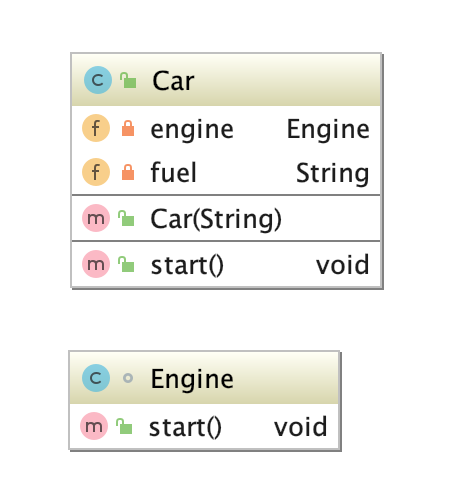
\includegraphics[width=5cm]{images/h5/oefening1.png}
  \label{fig:nested_classes}
\end{figure}

\end{oefening}

\subsection{Static nested class}

Je kan ervoor kiezen om een nested class als static te defini\"eren. In dat geval kan je objecten van de nested class aanmaken, zonder eerst een object van de outer class aan te maken. De static nested class heeft geen toegang tot non-static eigenschappen van de outer class.


\begin{lstlisting}
import java.util.ArrayList;
import java.util.List;

public class CPU {

	private List<Core> cores;
	private String manufacturer;

	public CPU(int numberOfCores, double clockspeed, String manufacturer) {
		cores = new ArrayList<>();
		for (int i = 0; i < numberOfCores; i++) {
			cores.add(new Core(clockspeed));
		}
		this.manufacturer = manufacturer;
	}

	public int getNumberOfCores() {
		return cores.size();
	}

	public static class Core {
		private double clockspeed;

		public Core(double clockspeed) {
			this.clockspeed = clockspeed;
		}

		public double getClockspeed() {
			return clockspeed;
		}
	}

	public static void main(String[] args) {
		CPU cpu = new CPU(4, 3.0, "AMD");
		System.out.println(cpu.getNumberOfCores());

		Core newCore = new CPU.Core(4.5);
		System.out.println(newCore.getClockspeed());
	}

}
\end{lstlisting}

\begin{oefening}
Maak nu van de inner class Engine een static nested class.
\end{oefening}

\subsubsection{Geneste enum}

Je kan ook een enum defini\"eren binnen een bestaande klasse.

\begin{lstlisting}
public class Document {
	private DocumentState state;
	private String name;

	public Document(String name) {
		this.name = name;
		state = DocumentState.CREATED;
	}

	public enum DocumentState {
		CREATED,
		ACCEPTED,
		REJECTED;
	}
}
\end{lstlisting}

Een enum is altijd een static nested class. Je hebt hier geen keuze. Omdat dit altijd static is, is het keywoord static redundant en zal je het ook nooit toevoegen.

\begin{figure}[H]
  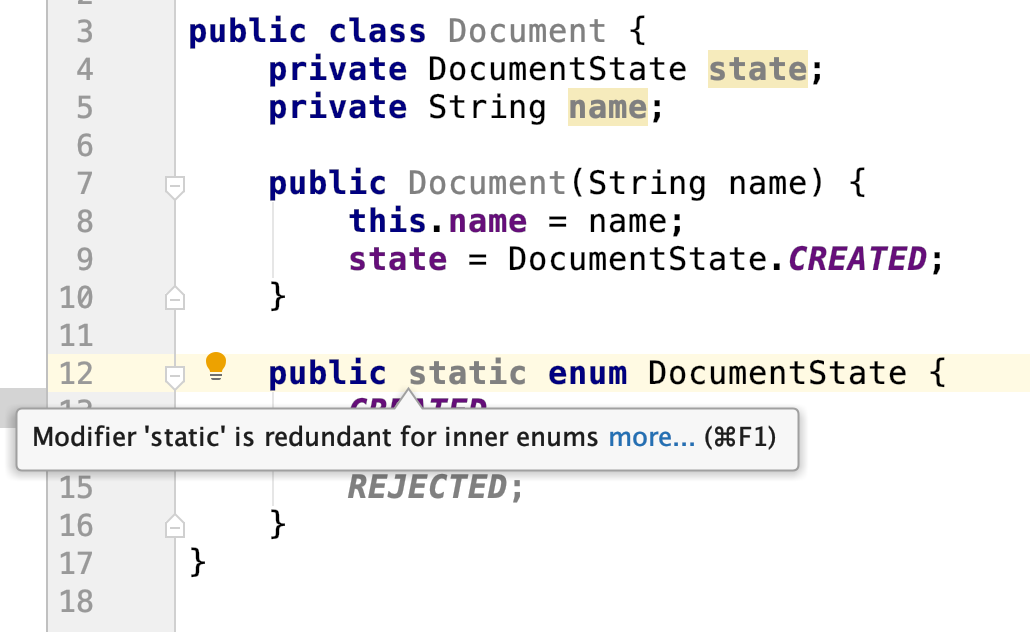
\includegraphics[width=8cm]{images/h5/nested_enum.png}
  \label{fig:nested_enum}
\end{figure}

\subsection{Local inner class}

In Java is het ook mogelijk om een klasse te defini\"eren in een methode. Dit noemen we een \textit{method local inner class}. Het bereik van deze lokale klasse is heel beperkt, enkel binnen de methode zelf kan je een object van deze klasse maken en gebruiken. Een method local inner class heeft dus hetzelfde bereik als een lokale variabele.
Je kan deze klasse dus nooit buiten de methode waarin hij gedefinieerd is, gebruiken.

\begin{lstlisting}
public class Person {
		private String name;
		private LocalDate dateOfBirth;

		public Person(String name, LocalDate dateOfBirth) {
			this.name = name;
			this.dateOfBirth = dateOfBirth;
		}

		public int getAge() {
			class PersonHelper {

				public int getAge() {
					return Period.between(dateOfBirth,
							LocalDate.now()).getYears();
				}
			}
			return new PersonHelper().getAge();
		}
}
\end{lstlisting}



\subsection{Anonymous inner class}

Een anonymous inner class is een inner klasse zonder naam waarvan  \'e\'en object wordt aangemaakt. Anonymous inner classes kunnen uitbreidingen zijn van bestaande klassen (zowel abstracte als concrete) of implementaties van interfaces. Ze worden dus gebruikt om methoden van bestaande klassen en interfaces te overschrijven of te implementeren, zonder ooit expliciet een subklasse te defini\"eren.  

\begin{lstlisting}
public class HorrorShow {

	interface Lethal {
		void kill();
		void destroy();
	}

	abstract class Vampire implements Lethal {
		private int bloodAvailable;

		@Override
		public void kill() {
			System.out.println("kill");
		}

		void drinkBlood(int amount) {
			bloodAvailable += amount;
		}

		@Override
		public String toString() {
			return "Vampire{" +
			         "class=" + this.getClass() + ", " +
					"bloodAvailable=" + bloodAvailable +
					'}';
		}
	}

	public void meetBarney() {
		Vampire barney = new Vampire() {
			@Override
			public void destroy() {
				drinkBlood(5);
				kill();
			}
		};
		System.out.println(barney);
		barney.destroy();
		System.out.println(barney);
	}


	public static void main(String[] args) {
		new HorrorShow().meetBarney();
	}
}
\end{lstlisting}

De output die verschijnt als je het bovenstaande programma uitvoert is:
\begin{verbatim}
Vampire{class=class be.pxl.ja.demo5.HorrorShow$1, bloodAvailable=0}
kill
Vampire{class=class be.pxl.ja.demo5.HorrorShow$1, bloodAvailable=5}
\end{verbatim}

We zien een anonymous inner class die de abstracte klasse Vampire implementeert. We hebben in 1 stap een nieuwe klasse en een object (barney) van deze klasse gemaakt, zonder de klasse te benoemen.

Als je de klasse van het object barney opvraagt en afdrukt krijg je het volgende resultaat.

\begin{verbatim}
class be.pxl.ja.demo5.HorrorShow$1
\end{verbatim}

De \$1 duidt op het feit dat barney een object is van de eerste anonymous inner class van de klasse HorrorShow.

\section{Functionele interfaces}

Herinner jij je de generieke interface Service$<$T$>$ uit het vorige hoofdstuk nog? Hier is hij nog een keer:

\begin{lstlisting}
public interface Service<T,U> {

	T execute(U arg);
}
\end{lstlisting}

Hier volgt de klasse CountService die de generieke interface Service implementeert.

\begin{lstlisting}
public class CountService implements Service<Integer, String> {

	@Override
	public Integer execute(String data) {
		return data.length();
	}
}
\end{lstlisting}

Een tenslotte nog een hoofdprogramma  waarin we gebruikmaken van een object van de klasse CountService.

\begin{lstlisting}
public class GenericServiceDemo {

	public static void main(String[] args) {

		CountService countService = new CountService();
		System.out.println(countService.execute("abcdefghijkl"));
	}
}
\end{lstlisting}

De klasse CountService bevat eigenlijk niet erg veel relevante informatie.  
We kunnen er dus ook voor kiezen om de implementatie van de klasse CountService te schrijven in een anonymous inner class.

\begin{lstlisting}
public class CountServiceDemo {

	public static void main(String[] args) {

		Service<Integer, String> countService  = new Service<>() {
			@Override
			public Integer execute(String data) {
				return data.length();
			}
		};
		System.out.println(countService.execute("abcdefghijkl"));
		System.out.println(countService.getClass());
	}
}
\end{lstlisting}

Eigenlijk staat in bovenstaande programma nog steeds overbodige code. De interface Service heeft maar 1 methode, dus voor die ene methode moeten we een implementatie voorzien. Verder weten we dankzij het datatype Service$<$Integer, String$>$ wat het datatype van onze parameter en het return-type moet zijn. Een lambda expressie maakt het nu mogelijk om bovenstaande code te vereenvoudigen zodat alle boilerplate-code verdwijnt. Hier is het resultaat.

\begin{lstlisting}
public class CountServiceDemo {

	public static void main(String[] args) {

		Service<Integer, String> countService  = (data) -> data.length();
		System.out.println(countService.getClass());
		System.out.println(countService.execute("abcdefghijkl"));
	}
}
\end{lstlisting}

De interface Service noemen we ook wel een \textbf{functionele interface} of \textbf{functional interface}. Een functionele interface is een interface met \'e\'en abstracte methode en de functionele interface kan dan ook gebruikt worden als datatype van een lambda expressie.

Functionele interfaces gaan we annoteren met @FunctionalInterface. Dit is niet verplicht, maar hierdoor zorg je ervoor dat er nooit een tweede abstracte methode aan de interface toegevoegd kan worden.  

\begin{lstlisting}
@FunctionalInterface
public interface Service<T,U> {

	T execute(U arg);
}
\end{lstlisting}

\section{Event handling}

JavaFX valt buiten de scope van deze cursus, maar toch tonen we hier een codefragment van de user interface van onze streaming service.

We kijken even naar de MainController, waarin afbeeldingen van de beschikbare content worden getoond.

\begin{lstlisting}
Image image = new Image("streamingservice/images/" + content.getImageUrl());
ImageView contentImage = new ImageView(image);
contentImage.setOnMouseClicked(new EventHandler<MouseEvent>() {
		@Override
		public void handle(MouseEvent mouseEvent) {
			openContentDetail(content);
		}
});
\end{lstlisting}

De contentImage is een cover-afbeelding van een film of serie. Als je op de afbeelding klikt, opent er een detailscherm met informatie van de film of serie.
Voor iedere contentImage voorzien we een object met implementatie van de generieke interface EventHandler.

\begin{figure}[H]
  \includegraphics[width=\linewidth]{images/h5/javadoc_eventhandler.png}
  \caption{Documentatie interface EventHandler}
  \label{fig:interface_eventhandler}
\end{figure}

De interface EventHandler is ook een functionele interface met \'e\'en methode handle().
De methode handle() wordt door het ImageView-object aangeroepen zodra een gebruiker op de afbeelding klikt.
We maken hier gebruik van een anonymous inner class.
Om het click-event af te handelen hebben we namelijk eerst een klasse nodig die de interface EventHandler implementeert. Daarna hebben we een object van deze klasse nodig, dat we aan het ImageView-object bekend kunnen maken en dat verantwoordelijk zal zijn voor het afhandelen van muisklik-events die op het ImageView-object worden uitgevoerd door de gebruiker. 
Omdat EventHandler een functionele interface is, kunnen we dit nu nog eenvoudiger schrijven door gebruik te maken van een lambda expressie.

\begin{lstlisting}
Image image = new Image("streamingservice/images/" + content.getImageUrl());
ImageView contentImage = new ImageView(image);
ontentImage.setOnMouseClicked((mouseEvent) -> openContentDetail(content));
\end{lstlisting}

\section{Standaard functionele interfaces}

Sinds Java 8 beschikken we over verschillende functionele interfaces om lambda expressies te schrijven. Deze functionele interfaces vind je terug in het package \textit{java.util.function}.

\subsection{Verschillende manieren om lambda expressies te schrijven}

Lambda expressies vind je terug in verschillende vormen: met en zonder parameters, met 1 instructies of met meerdere instructies,... Hier zijn alvast enkele voorbeelden.

\begin{lstlisting}
import java.util.function.IntBinaryOperator;
import java.util.function.IntConsumer;
import java.util.function.IntUnaryOperator;
import java.util.function.Supplier;

public class DifferentFlavoursDemo {

	public static void main(String[] args) {

		Supplier<Integer> always5 = () -> 5;
		IntUnaryOperator sqrt = (int x) -> x * x;
		IntUnaryOperator plus5 = x -> x + 5;
		IntBinaryOperator sumSqrt = (x, y) -> sqrt.applyAsInt(x) + sqrt.applyAsInt(y);
		IntConsumer printInBox = x -> {
			int length = String.valueOf(x).length();
			System.out.println("*".repeat(length + 2));
			System.out.println("*"+ x + "*");
			System.out.println("*".repeat(length + 2));
		};

		System.out.println(always5.get());
		System.out.println(sqrt.applyAsInt(5));
		System.out.println(plus5.applyAsInt(10));
		System.out.println(sumSqrt.applyAsInt(7, 5));
		printInBox.accept(1234567);
	}
}
\end{lstlisting}

\begin{verbatim}
5
25
15
74
*********
*1234567*
*********
\end{verbatim}

\begin{oefening}
Zoek de documentatie van de verrschillende functionele interfaces die in bovenstaand voorbeeld DifferentFlavoursDemo gebruikt worden.
\end{oefening}

In de volgende paragrafen bestuderen we enkele generieke functionele interfaces in detail.

\subsection{Predicate$<$T$>$}

Predicate$<$T$>$ is een veelgebruikte functionele interface die een functie \textbf{test} voorziet met \'e\'en parameter met datatype T die een boolean-waarde (true of false) teruggeeft. Naast de abstracte methode test zijn er ook nog enkele default functies voorzien om Predicates te combineren met and, or en negate (not).

\begin{table}[h!]
\centering
\begin{tabularx}{\textwidth}{| l | X |}
 \hline
 Methode & Betekenis\\ 
 \hline
 boolean test(T t) &	It evaluates this predicate on the given argument.\\
 \hline
 default Predicate$<$T$>$ and(Predicate$<$? super T$>$ other)	& It returns a composed predicate that represents a short-circuiting logical AND of this predicate and another. When evaluating the composed predicate, if this predicate is false, then the other predicate is not evaluated.\\
\hline
 default Predicate$<$T$>$ or(Predicate$<$? super T$>$ other) &	It returns a composed predicate that represents a short-circuiting logical OR of this predicate and another. When evaluating the composed predicate, if this predicate is true, then the other predicate is not evaluated.\\
  \hline
 default Predicate$<$T$>$ negate()	& It returns a predicate that represents the logical negation of this predicate.\\
  \hline
\end{tabularx}
\end{table}

\begin{lstlisting}
import java.util.ArrayList;
import java.util.List;
import java.util.function.Predicate;

public class PrincessNames {

	private List<String> names = new ArrayList<>();

	public PrincessNames() {
		names.add("Snow White");
		names.add("Cinderella");
		names.add("Aurora");
		names.add("Ariel");
		names.add("Belle");
		names.add("Jasmine");
		names.add("Pocahontas");
		names.add("Mulan");
		names.add("Tiana");
		names.add("Rapunzel");
		names.add("Merida");
		names.add("Moana");
	}

	public void filterNames(Predicate<String> filter) {
		for (String name : names) {
			if (filter.test(name)) {
				System.out.println(name + " is valid!");
			}
		}
	}
}
\end{lstlisting}

\begin{lstlisting}
import java.util.function.Predicate;

public class DemoPrincessNames {

	public static void main(String[] args) {
		PrincessNames princessNames = new PrincessNames();
		System.out.println("Filter 1");
		princessNames.filterNames((n) -> n.contains("o"));
		System.out.println("Filter 2");
		Predicate<String> length5 = (n) -> n.length() == 5;
		princessNames.filterNames(length5);
		System.out.println("Filter 3");
		Predicate<String> startsWithA = (n) -> n.startsWith("A");
		princessNames.filterNames(startsWithA.and(length5));
	}
}
\end{lstlisting}

\begin{verbatim}
Filter 1
Snow White is valid!
Aurora is valid!
Pocahontas is valid!
Moana is valid!
Filter 2
Ariel is valid!
Belle is valid!
Mulan is valid!
Tiana is valid!
Moana is valid!
Filter 3
Ariel is valid!
\end{verbatim}

\subsection{Function$<$T, R$>$}

De generieke functionele interface Function voorziet een functie apply die een argument aanneemt en een resultaat produceert. Er zijn dus 2 verschillende generieke datatypes:
\begin{itemize}
\item T: het type van het argument 
\item R het type van het resultaat
\end{itemize}

\begin{lstlisting}
import java.util.Arrays;
import java.util.List;
import java.util.function.Function;

public class Weights {

	private List<Double> weigths = Arrays.asList(87.5, 87.3, 88.1, 87.7, 87.4, 86.6);

	public void roundWeights(Function<Double, Integer> rounder) {
		for (double weight : weigths) {
			int intValue = rounder.apply(weight);
			System.out.println("Rounded " + weight + ": " + intValue);
		}
	}
}
\end{lstlisting}

\begin{lstlisting}
public class DemoFunction {

	public static void main(String[] args) {
		Weights weights = new Weights();
		System.out.println("Rounding down");
		weights.roundWeights(d -> Double.valueOf(Math.floor(d)).intValue());

		System.out.println("Rounding up");
		weights.roundWeights(d -> Double.valueOf(Math.ceil(d)).intValue());
	}
}
\end{lstlisting}

\begin{verbatim}
Rounding down
Rounded 87.5: 87
Rounded 87.3: 87
Rounded 88.1: 88
Rounded 87.7: 87
Rounded 87.4: 87
Rounded 86.6: 86
Rounding up
Rounded 87.5: 88
Rounded 87.3: 88
Rounded 88.1: 89
Rounded 87.7: 88
Rounded 87.4: 88
Rounded 86.6: 87
\end{verbatim}

\subsection{Consumer$<$T$>$}

De generieke functionele interface Consumer$<$T$>$ bevat een functie accept die \'e\'en argument aanneemt. De functie geeft geen resultaat terug. 

\begin{lstlisting}
import java.util.Arrays;
import java.util.List;
import java.util.function.Consumer;

public class Weights {

	private List<Double> weigths = Arrays.asList(87.5, 87.3, 88.1, 87.7, 87.4, 86.6);

	public void consumeWeights(Consumer<Double> consumer) {
		for (double weight : weigths) {
			consumer.accept(weight);
		}
	}
}
\end{lstlisting}

\begin{lstlisting}
public class DemoConsumer {

	public static void main(String[] args) {
		Weights weights = new Weights();

		System.out.println("Displaying");
		weights.consumeWeights(d -> System.out.println(String.format("%.2f", d)));
	}
}
\end{lstlisting}

\begin{verbatim}
87,50
87,30
88,10
87,70
87,40
86,60
\end{verbatim}

\section{Method reference}

Method references zijn een speciaal type lambda expressies. Ze worden gebruikt om lambda expressies te vereenvoudigen door te verwijzen naar een bestaande methode, zonder dat je expliciet de parameters moet invullen.

Er zijn 4 soorten methodes in Java:
\begin{itemize}
\item static methods
\item constructoren
\item instance methods
\end{itemize}

\subsection{Static methods}
Syntax: 
\begin{verbatim}
ClassName::staticMethod
\end{verbatim}

\begin{lstlisting}
IntBinaryOperator min = (x, y) -> Math.min(x, y);
IntBinaryOperator max = Math::max;

System.out.println(min.applyAsInt(-3, 17));
System.out.println(max.applyAsInt(-3, 17));
\end{lstlisting}



\subsection{Instance method (unbounded)}
Syntax:
\begin{verbatim}
ClassName::instanceMethod
\end{verbatim}

\begin{lstlisting}
Function<String, String> toUpperCase = s -> s.toUpperCase();
Function<String, String> toLowerCase = String::toLowerCase;
System.out.println(toUpperCase.apply("abcdef"));
System.out.println(toLowerCase.apply("ABCDEF"));
\end{lstlisting}

\subsection{Instance method (bounded)}

Syntax:
\begin{verbatim}
instance::instanceMethod
\end{verbatim}

De klasse Random voorziet 2 versies van de methode nextInt(): een eerste versie zonder parameter en een tweede versie met \'e\'en parameter, de bovengrens. Dit principe noemen we methode overloading. Aan de hand van de functionele interface die je implementeert, kan je nu de gewenste methode als en lambda functie schrijven. Hier illustreren we hoe je deze lambda functie ook nog eens verkort kan schrijven door gebruik te maken van method reference.

\begin{lstlisting}
Random random = new Random();
IntSupplier randomInt = random::nextInt;
IntUnaryOperator randomIntWithBound = random::nextInt;
System.out.println(randomInt.getAsInt());
System.out.println(randomIntWithBound.applyAsInt(12));
\end{lstlisting}

\subsection{Constructor}

Je kan ook voor een constructor een method reference maken. De syntax van de method reference voor een constructor ziet er als volgt uit.

\begin{verbatim}
ClassName::new
\end{verbatim}

\begin{lstlisting}
System.out.println("Constructor");
Supplier<Random> randomCreator = Random::new;
Random random = randomCreator.get();
Function<Integer, ArrayList<Movie>> movieListCreator = ArrayList::new;
ArrayList<Movie> movieList = movieListCreator.apply(120);
\end{lstlisting}

Wanneer je gebruikmaakt van de movieListCreator (door de methode apply aan te roepen) moet je een integer-waarde als parameter geven. 
Je roept op dat ogenblik de constructor met 1 int-parameter (initialCapacity) uit de klasse ArrayList aan.

\begin{verbatim}
ArrayList(int initialCapacity)
Constructs an empty list with the specified initial capacity.
\end{verbatim} 
\vspace{4cm}

\section{Oefeningen}

\begin{oefening}
De klasse \textit{NumberMachine} bevat een lijst van integers die verwerkt moeten worden. De klasse heeft ook een methode \textit{processNumbers}. Deze methode staat momenteel nog in commentaar, pas dit even aan zodat de methode wel beschikbaar is. De methode processNumbers zal de lijst van integers inspecteren en afhankelijk hiervan
een selectie van getallen samenzetten in een String (met telkens een streepje tussen de int-waarden: bv.
1-2-3). Deze samengestelde String wordt teruggegeven door de methode processNumbers. De manier waarop de integers verwerkt worden,
wordt bepaald door een object dat de interface \textit{NumberFilter} implementeert.\\

Schrijf de functionele interface \textit{NumberFilter} met als enige methode boolean check(int number).\\

Voeg in de klasse \textit{NumberSelector} een member-variabele toe met als type NumberMachine. Implementeer vervolgens de constructor.\\ 

Implementeer in de klasse  \textit{NumberSelector} eerst de methode \textit{showEvenNumbers()}. Zorg dat deze methode de methode processNumbers van
het NumberMachine object oproept en de NumberFilter op een manier implementeert zodat enkel even
getallen afgedrukt worden. Doe dit door gebruik te maken van een anonieme geneste klasse.
Test nadien je code met de EvenNumbersTest.\\

Implementeeer nu de tweede methode: \textit{showNumbersAbove()}, eveneens in de NumberSelector klasse. Deze
methode krijgt een integer als parameter mee en zal opnieuw de processNumbers methode gebruiken,
maar deze keer om enkel getallen af te drukken die boven het meegegeven getal liggen. Definieer de
instantie van NumberFilter met behulp van een lambda expressie.
Test nadien je code met de NumbersAboveTest.\\

Implementeer tenslotte de derde methode \textit{printHexNumbers()}. Deze methode moet de integers tonen in
hexadecimale notatie. Hier kan je geen gebruik maken
maken van de NumberFilter, omdat deze een boolean moet returnen. Maak voor deze oefening een
methode \textit{convertNumbers} in \textit{NumberMachine}, die een standaard functionele interface gebruikt die
geschikt is voor deze methode. De methode geeft de hexadecimale waarden in een String als
returnwaarde terug. De waarden zijn opnieuw gescheiden door een streepje -. Gebruik tenslotte de
methode convertNumbers in combinatie met een lambda expressie om het gewenste resultaat te
bekomen.
Test je code opnieuw met de HexNotationTest.
\end{oefening}

\begin{oefening}
De klasse \textit{VideoGame} is reeds gegeven. Bestudeer deze klasse even. \\

Implementeer in de klasse \textit{GameCollection} de methode \textit{addGame}, die een VideoGame-object als argument krijgt en dit object gaat
toevoegen aan de verzameling van VideoGame-objecten.\\

Voeg nu een methode \textit{selectGames} toe aan de GameCollection klasse. Deze methode krijgt als
argument een object dat één of andere filter implementeert. Zoek zelf in je cursus of op internet welke
standaard functionele interface je hier best voor kan gebruiken. De methode selectGames zal door de
lijst met games in de collectie lopen en alle VideoGames die voldoen aan de eisen van de meegegeven
filter, toevoegen aan een nieuwe ArrayList van VideoGames. Deze ArrayList is het resultaat en wordt
teruggegeven als return waarde door deze methode.\\

Implementeer nu de methoden van de klasse \textit{GameBrowser}. 
De methode showGamesForSearch krijgt een String  als
parameter en gaat daarmee de games uit de collectie filteren die deze String in hun naam bevatten. Dit
doe je door een gepaste implementatie van het filter object te voorzien en deze mee te geven aan de
selectGames methode van GameCollection. Doe dit in deze methode met behulp van een anonieme geneste klasse.
Geef nadien de resulterende ArrayList van VideoGames terug als return waarde.
Je kan de methode controleren met de GamesSearchTest.\\

Implementeer vervolgens de methode \textit{showFreeGames}. Roep daarvoor opnieuw de methode selectGames
uit GameCollection aan en voorzie een gepaste implementatie van de filter, maar deze keer aan de hand
van een lambda expressie. Geef nadien de resulterende ArrayList van VideoGames terug als return waarde.
Controleren kan je met de FreeGamesTest.\\

Implementeer tenslotte de methode \textit{showGamesInGenre}. Deze heeft een String genre als
parameter en gaat daarmee alle games in de collectie selecteren die dat genre bevatten. Verder werkt
de methode analoog aan de methode showFreeGames. (werk opnieuw met een lambda expressie)
Check of alles naar behoren werkt met de GamesGenreTest.
\end{oefening}

\chapter{Streams}

\begin{summary}
De Stream API van Java biedt een elegante manier om collections te manipuleren. De belangrijkste interface uit de API is Stream$<$T$>$. Als Java ontwikkelaar gebruik je voornamelijk deze interface die alle implementatie-details verbergt. Bij het ontwerpen van de Stream API is, naast het aanbieden van een elegante en eenvoudige API, ook veel aandacht besteed aan performantie. 
\end{summary}

\section{External en internal iterators}

Veronderstel dat we een verzameling met Movie-objecten hebben: \textit{movies}. We willen nu graag weten hoeveel actiefilms er in onze verzameling zitten.

Hier is de code om dit te berekenen.

\begin{lstlisting}
int count = 0;
for (Movie movie: movies) {
    if (movie.getGenre() == Genre.ACTION) {
        count++;
    }
}
\end{lstlisting}

Bovenstaand voorbeeld bevat veel boilerplate code en daarnaast hebben we ook een external iterator. 

Een stream maakt het mogelijk om op een functionele manier complexe bewerkingen uit te voeren op een verzameling.
We kunnen bovenstaande code schrijven met behulp van een stream. Onze external iterator verdwijnt en we krijgen een internal iterator in de plaats.

\begin{lstlisting}
int count = movies.stream().filter(m -> m.getGenre() == Genre.ACTION).count();
\end{lstlisting}

Een stream bestaat uit 3 delen: een (data) bron, intermediate operations (tussentijdse bewerkingen) en een terminal operation (eindbewerking). In ons voorbeeld is de verzameling movies de bron, vervolgens hebben we een intermediate operation \textit{filter} en tenslotte een terminal operation \textit{count}.

\begin{figure}[H]
  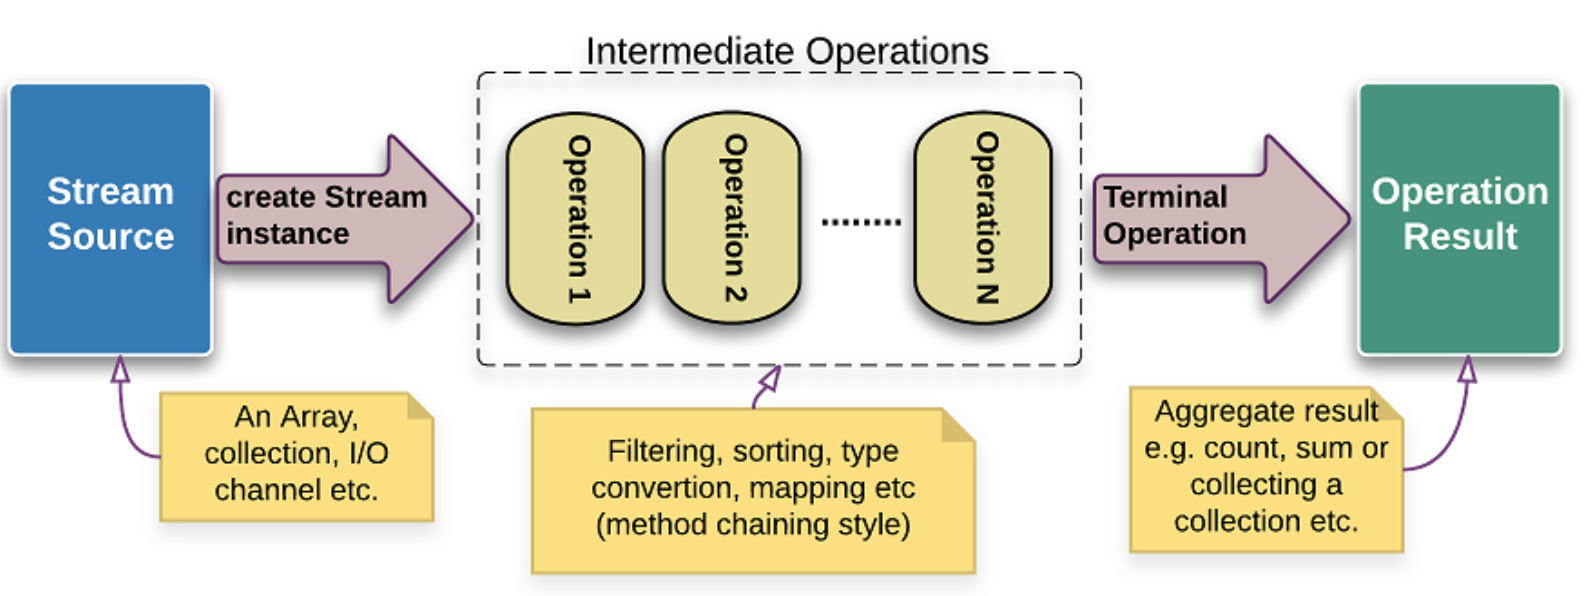
\includegraphics[width=\linewidth]{images/h6/stream_pipeline.png}
  \caption{Stream pipeline (logicbig.com)}
  \label{fig:stream_of}
\end{figure}


De intermediate operators verwerken de elementen van de stream \'e\'en voor \'e\'en. Alle intermediate operations zijn lui (lazy), ze worden enkel uitgevoerd als de stream wordt afgesloten door een terminal operation.

De internal iterator geniet meestal de voorkeur. Internal iterations kunnen korter geschreven worden en zijn daardoor ook makkelijker lees- en onderhoudbaar. Toch zijn er situaties, zoals wanneer je 2 verzamelingen gelijktijdig manipuleert, dat je kiest voor een external iterator.

\begin{figure}[H]
  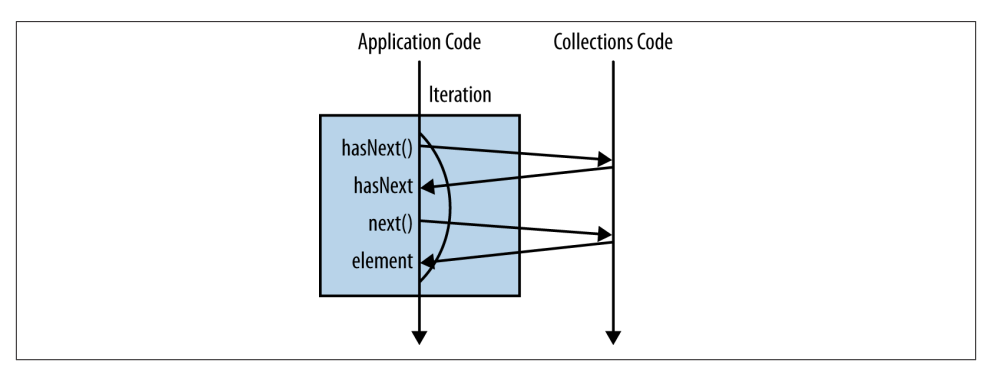
\includegraphics[width=\linewidth]{images/h6/external_iteration.png}
  \caption{External iteration}
  \label{fig:external_iteration}
\end{figure}

\begin{figure}[H]
  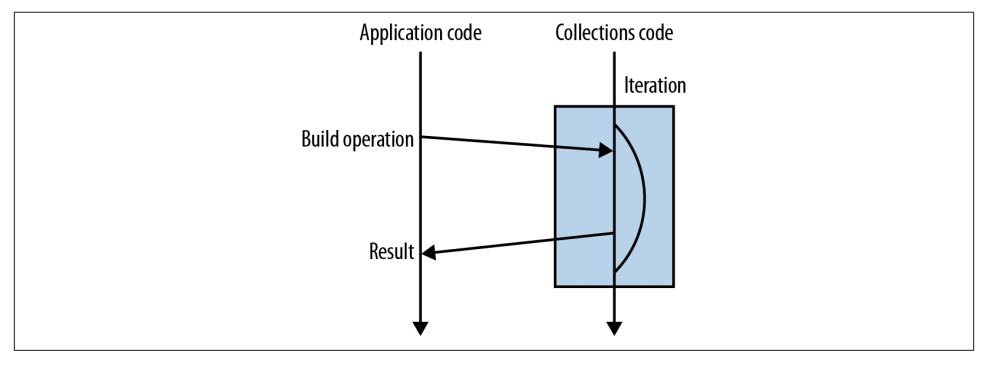
\includegraphics[width=\linewidth]{images/h6/internal_iteration.png}
  \caption{Internal iteration}
  \label{fig:internal_iteration}
\end{figure}

\section{Intermediate en terminal operations}

\subsection{Terminal operation .collect()}

\begin{lstlisting}
import java.util.List;
import java.util.stream.Collectors;
import java.util.stream.Stream;

public class DemoCollect {

	public static void main(String[] args) {

		List<String> theBeatles = 
				Stream.of("John Lennon", "Paul McCartney", "George Harrison", "Ringo Starr")
				.collect(Collectors.toList());
		System.out.println(theBeatles);
	}

}
\end{lstlisting}

Een stream is geen datastructuur of verzameling. Je moet een stream zien als een reeks objecten. E\'en van de manieren om zo'n reeks of stream te bouwen is met de static methode \textit{of} van de interface Stream.

\begin{figure}[H]
  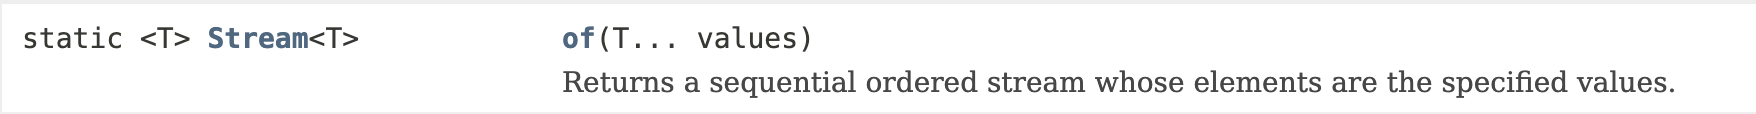
\includegraphics[width=\linewidth]{images/h6/stream_of.png}
  \caption{Static methode of() in de interface Stream}
  \label{fig:stream_of}
\end{figure}

Door gebruik te maken van de operation \textit{collect(Collectors.toList())} kunnen we de objecten uit de stream verzamelen in een List.

\subsection{Intermediate operation .filter()}

Wanneer je bepaalde elementen uit een stream wil selecteren, gebruik je een filter. 

\begin{figure}[H]
  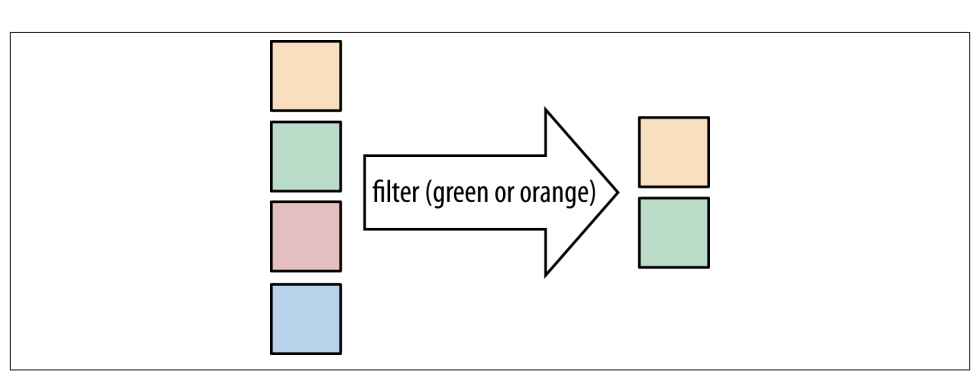
\includegraphics[width=\linewidth]{images/h6/illustration_filter.png}
  \caption{Filter operation}
  \label{fig:filter_operation}
\end{figure}

\begin{figure}[H]
  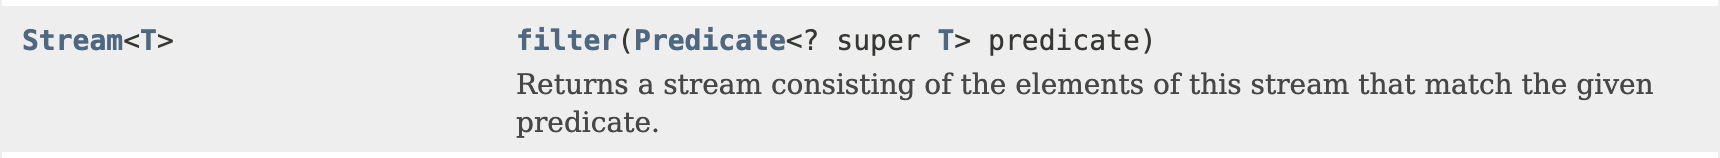
\includegraphics[width=\linewidth]{images/h6/stream_filter.png}
  \caption{Methode filter() in de interface Stream}
  \label{fig:stream_filters}
\end{figure}

Aan de hand van een Predicate wordt beslist welke elementen geselecteerd worden. 

In het onderstaande voorbeeld selecteren we de even getallen uit de verzameling numbers.

\begin{lstlisting}
List<Integer> numbers = Arrays.asList(1,2,3,4,5);

List<Integer> evenNumbers = numbers.stream()
				.filter(n -> n%2  == 0)
				.collect(Collectors.toList());
				
assertEquals(Arrays.asList(2,4), evenNumbers);
\end{lstlisting}

Nog een voorbeeld.

\begin{lstlisting}
List<String> animals = Stream.of("zebra", "dog", "dolphine")
				.filter(a -> a.contains("o"))
				.collect(Collectors.toList());

assertEquals(Arrays.asList("dog", "dolphine"), animals);
\end{lstlisting}

Alle String-objecten die een ``o'' bevatten mogen in de stream aanwezig blijven.

Merk op dat de functie filter() een intermediate operation is. De bewerking heeft als return-type Stream. We bouwen als het ware een pipeline. De filter()-operation is ook lazy en zal pas effectief uitgevoerd worden als er een terminal-operation aanwezig is.

Hier volgt nog een voorbeeld met een verzameling met objecten van een zelfgeschreven klasse Participant.

\begin{lstlisting}
public class Participant {
	private String name;
	private int points;

	public Participant(String name, int points) {
		this.name = name;
		this.points = points;
	}

	public int getPoints() {
		return points;
	}

	public String getName() {
		return name;
	}
}
\end{lstlisting}

\begin{lstlisting}
Participant john = new Participant("John P.", 15);
Participant sarah = new Participant("Sarah M.", 200);
Participant charles = new Participant("Charles B.", 150);
Participant mary = new Participant("Mary T.", 1);

List<Participant> participants = Arrays.asList(john, sarah, charles, mary);

List<Participant> over100Points = participants.stream()
     .filter(p -> p.getPoints() > 100)
     .collect(Collectors.toList());

assertEquals(Arrays.asList(sarah, charles), over100Points);
\end{lstlisting}

Je kan ook meerdere criteria gebruiken in een filter. Je kan in het Predicate de verschillende criteria samenvoegen via boolean operatoren.

\begin{lstlisting}
List<Participant> selection = participants.stream()
    .filter(p -> p.getPoints() > 100 && p.getName().startsWith("S"))
    .collect(Collectors.toList());
    
assertEquals(Collections.singletonList(sarah), selection);
\end{lstlisting}

Daarnaast kan je ook gebruikmaken van methodes als ``or'',  ``and'' en ``negate'' uit de interface Predicate.
		
\begin{lstlisting}
Predicate<Participant> over100Points = p -> p.getPoints() > 100;
Predicate<Participant> startingWithS = p -> p.getName().startsWith("S");

List<Participant> selection = participants.stream()
    .filter(over100Points.and(startingWithS))
    .collect(Collectors.toList());

assertEquals(Collections.singletonList(sarah), selection);
\end{lstlisting}

\subsection{Terminal operation .forEach()}

De methode .forEach() is een terminal operation en aanvaardt een implementatie van de functionele interface Consumer als parameter. Deze Consumer beschrijft een actie die met ieder element van de verzameling uitgevoerd zal worden.

\begin{figure}[H]
  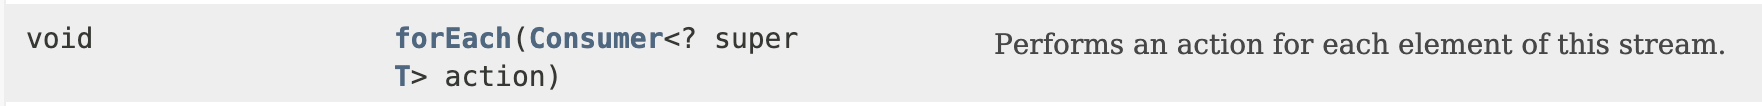
\includegraphics[width=\linewidth]{images/h6/stream_forEach.png}
  \caption{Methode forEach() in de interface Stream}
  \label{fig:stream_foreach}
\end{figure}

\begin{lstlisting}
public class DemoForEach {

	public static void main(String[] args) {
		Participant john = new Participant("John P.", 15);
		Participant sarah = new Participant("Sarah M.", 200);
		Participant charles = new Participant("Charles B.", 150);
		Participant mary = new Participant("Mary T.", 1);

		List<Participant> participants = Arrays.asList(john, sarah, charles, mary);

		participants.stream()
		    .filter(p -> p.getPoints() >= 200)
		    .forEach(System.out::println);

		System.out.println("* All participants *");

		participants.forEach(System.out::println);
	}
}
\end{lstlisting}

Iedere Collection biedt via de interface Iterable ook een forEach methode aan. Met beide forEach functies kan je hetzelfde resultaat bereiken.

\begin{lstlisting}
participants.forEach(System.out::println);
participants.stream().forEach(System.out::println);
\end{lstlisting}

Toch gaat in dit geval onze voorkeur uit naar de eerste optie. Omdat we hier itereren over alle elementen is de stream overbodig.


\subsection{Intermediate operation .map()}

Als je een functie hebt om objecten van \'e\'en datatype te transformeren naar een ander datatype, dan kan je met de bewerking .map(), deze functie loslaten op alle objecten van een stream. 

\begin{figure}[H]
  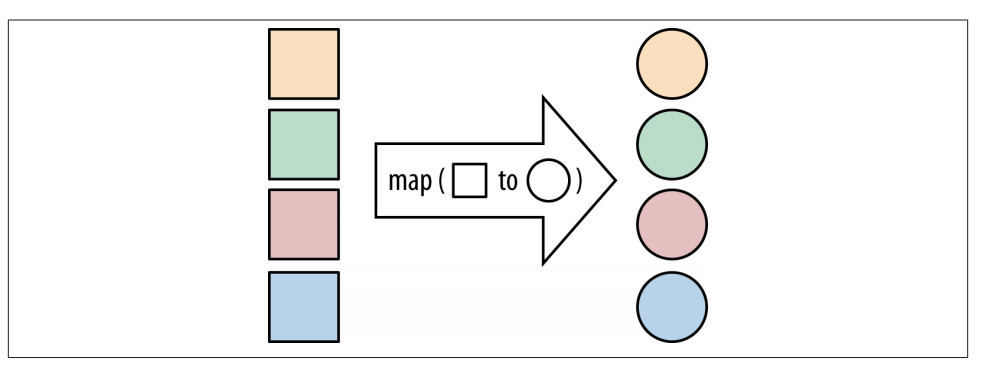
\includegraphics[width=\linewidth]{images/h6/illustration_map.png}
  \caption{Map operation}
  \label{fig:stream_foreach}
\end{figure}

\begin{figure}[H]
  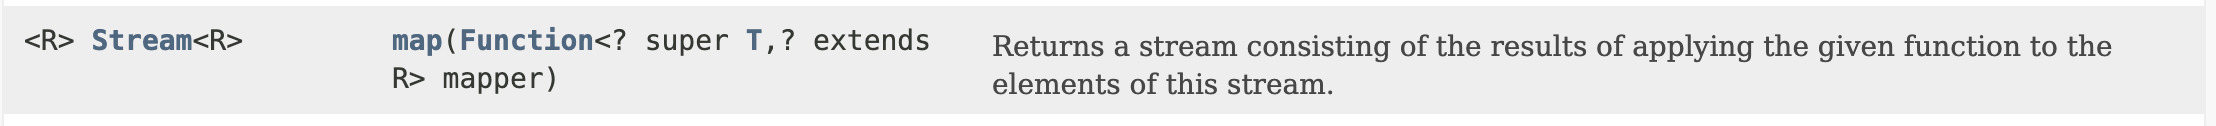
\includegraphics[width=\linewidth]{images/h6/stream_map.png}
  \caption{Methode map() in de interface Stream}
  \label{fig:stream_foreach}
\end{figure}

Map is een lazy operator. Zonder terminal operator zal de meegegeven functie niet uitgevoerd worden, en zal je dus ook geen resultaat krijgen. De functie die je meegeeft aan map is een implementatie van de generieke functionele interface Function$<$T,R$>$.

Hier volgen een twee voorbeelden. In het eerste voorbeeld wijzigt het datatype van de elementen van de stream niet. In het tweede voorbeeld wordt ieder String-object in de stream vervangen door een Integer-waarde.

\begin{lstlisting}
List<String> animals = Stream.of("zebra", "dog", "dolphine")
				.map(String::toUpperCase)
				.collect(Collectors.toList());

assertEquals(Arrays.asList("ZEBRA", "DOG", "DOLPHINE"), animals);
\end{lstlisting}

\begin{lstlisting}
List<Integer> lengths = Stream.of("zebra", "dog", "dolphine")
				.map(String::length)
				.collect(Collectors.toList());

assertEquals(Arrays.asList(5, 3, 8), lengths);
\end{lstlisting}

\subsection{Intermediate operation .sorted()}

Wanneer je de intermediate operation sorted() toevoegt aan een stream, worden de elementen in de stream gesorteerd. Zonder parameter zal sorted() de natuurlijke sortering gebruiken. Voor objecten van een zelfgeschreven klasse zorg je er dus voor dat de interface Comparable ge\"implementeerd wordt.

Het is ook mogelijk dat je aan de functie sorted() een parameter meegeeft waarmee je een andere volgorde kan afdwingen. In het tweede voorbeeld gebruiken we niet de natuurlijke (alfabetische) volgorde, maar worden de woorden van lang naar kort gesorteerd.


\begin{lstlisting}
List<String> sortedList = Stream.of("zebra", "dog", "dolphine")
				.sorted()
				.collect(Collectors.toList());

assertEquals(Arrays.asList("dog", "dolphine", "zebra"), sortedList);
\end{lstlisting}

\begin{lstlisting}
List<String> sortedList = Stream.of("zebra", "dog", "dolphine")
				.sorted((x, y) -> y.length() - x.length())
				.collect(Collectors.toList());
		
assertEquals(Arrays.asList("dolphine", "zebra", "dog"), sortedList);
\end{lstlisting}

\subsection{Intermediate operation .distinct()}

De operation .distinct() zorgt ervoor dat de elementen in de stream uniek zijn. Elementen die meermaals voorkomen worden verwijderd. Het is de implementatie van de equals() methode (en dus ook hashCode()) van een klasse die beslist of de elementen uniek zijn of niet.

\begin{lstlisting}
List<String> withoutDoubles = Stream.of("zebra", "dog", "zebra", "dolphine")
    .distinct()
    .collect(Collectors.toList());
    
assertEquals(3, withoutDoubles.size());
\end{lstlisting}

\subsection{Intermediate operation .limit()}

De operation .limit() heeft 1 parameter die het maximaal toegelaten elementen in de stream geeft.
De stream wordt dus als het ware afgekapt.

\begin{lstlisting}
List<String> animals = Stream.of("zebra", "dog", "elephant", "camel", "cat", "fish","dolphine")
    .limit(4)
    .collect(Collectors.toList());
assertEquals(4, animals.size());
\end{lstlisting}

Met de methode iterate kunnen we een oneindige stream maken. Dankzij de limit(5) worden slechts de eerste 5 nummers gegenereerd.

\begin{lstlisting}
List<Integer> numbers = Stream.iterate(1, n -> n + n)
    .limit(5)
    .collect(Collectors.toList());

assertEquals(Arrays.asList(1,2,4,8,16), numbers);
\end{lstlisting}


\subsection{Intermediate operation peek()}

De intermediate operation peek kan gebruikt worden om je pipeline te debuggen. Als je wilt controleren welke elementen er op een gegeven moment in de pipeline zitten, dan voeg je peek toe. Zolang je geen terminal operation hebt toegevoegd zal ook peek geen resultaat laten zien.

\begin{lstlisting}
Stream.of("one", "two", "three", "four")
  .filter(e -> e.length() > 3)
  .peek(e -> System.out.println("Filtered value: " + e))
  .map(String::toUpperCase)
  .peek(e -> System.out.println("Mapped value: " + e))
  .collect(Collectors.toList());
\end{lstlisting}

Je kan de operation peek() verder ook handig gebruiken om de elementen van je stream aan te passen.

\begin{lstlisting}
Stream<User> userStream = Stream.of(new User("Alice"), new User("Bob"), new User("Chuck"));
userStream.peek(u -> u.setName(u.getName().toLowerCase()))
  .forEach(System.out::println);
  \end{lstlisting}


\subsection{Terminal operation .count()}

\begin{lstlisting}
long over100Points = participants.stream().filter(p -> p.getPoints() > 100).count();

assertEquals(2, over100Points);
\end{lstlisting}
		
De terminal operation count gebruik je om het aantal elementen in de stream te tellen.
Indien je geen gebruik maakt van intermediate operations gebruik je de methode size() van je collection om het aantal elementen te achterhalen.

\begin{lstlisting}
System.out.println("Number of participants: " + participants.size());
\end{lstlisting}
		
\section{Intstream, LongStream en DoubleStream}
	
Er zijn ook een aantal afgeleide interfaces van de interface Stream. Deze bieden extra functionaliteit aan. Zo hebben we bijvoorbeeld de interface IntStream, die speciaal ontworpen is voor streams met gehele getallen. Deze stream bevat elementen met datatype \textit{int}. Naast IntStream hebben we ook de interfaces DoubleStream en LongStream. Al deze interfaces bevatten de methoden sum(), min(), max() en average(). 

\subsection{sum()}

Met de operation sum kan je eenvoudig de som berekenen van alle elementen in je stream.

\begin{lstlisting}
long totalPoints = participants.stream().mapToInt(Participant::getPoints).sum();

assertEquals(366, totalPoints);
\end{lstlisting}
		

\subsection{range() en rangeClosed()}
		
De static methoden range() en rangeClosed() zijn beschikbaar in de interfaces java.util.stream.IntStream en java.util.stream.LongStream. Je kan ze gebruiken om een stream te cre\"eren met gehele getallen vanaf een init\"ele waarde tot een stop waarde.
\begin{figure}[H]
  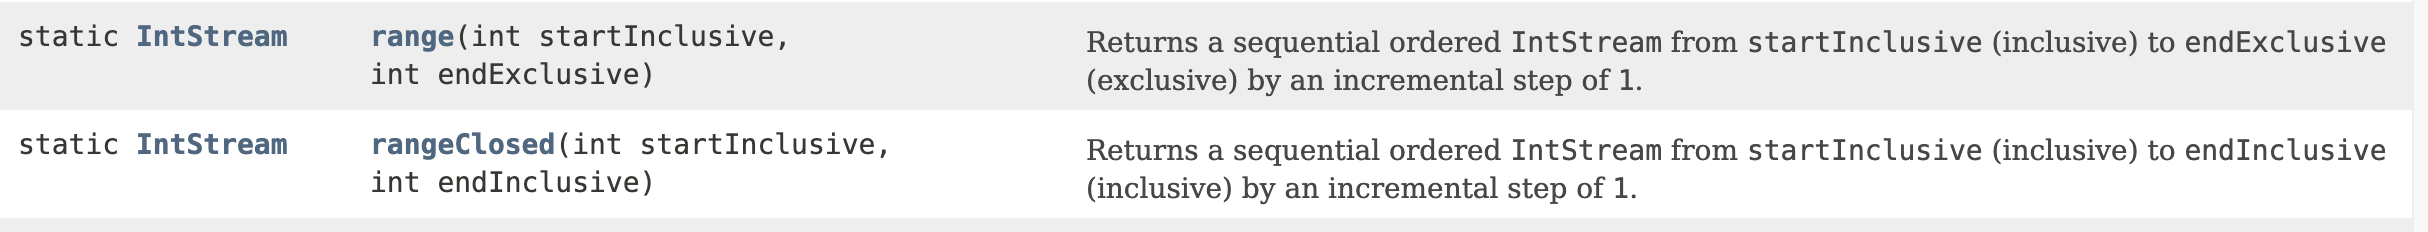
\includegraphics[width=\linewidth]{images/h6/intstream_range.png}
  \caption{Aanmaken van IntStream met range() of rangeClosed()}
  \label{fig:stream_foreach}
\end{figure}

\begin{lstlisting}
long count = IntStream.rangeClosed(10, 20).count();

assertEquals(11, count);
\end{lstlisting}

\subsection{min(), max() en average()}

\begin{figure}[H]
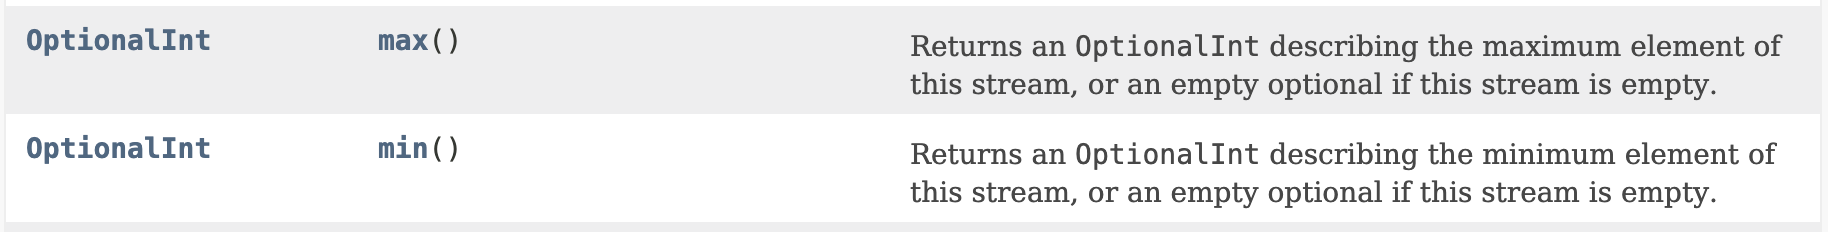
\includegraphics[width=\linewidth]{images/h6/intstream_max_min.png}
\caption{min() en max() uit de interface IntStream}
\label{fig:instream_min_max}
\end{figure}

\begin{figure}[H]
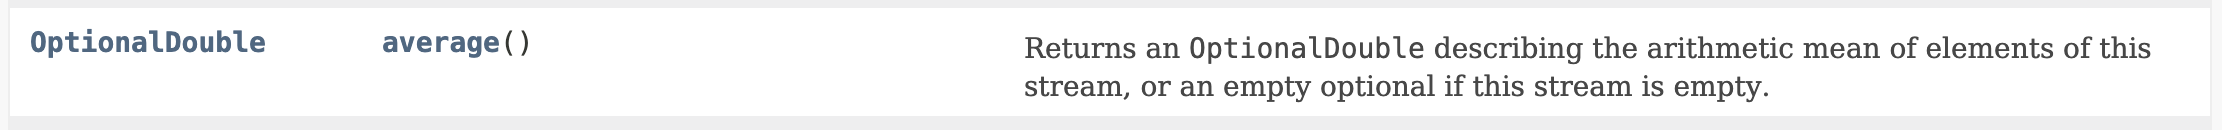
\includegraphics[width=\linewidth]{images/h6/intstream_average.png}
\caption{average() uit de interface IntStream}
\label{fig:instream_average}
\end{figure}

Merk op dat de methoden max() en min() een object van de klasse OptionalInt als return-type hebben. De methode average() heeft OptionalDouble als return-type. 

\begin{oefening}
Zoek de klasse OptionalInt en OptionalDouble op in de Java documentatie.
\end{oefening}

In de documentatie vind je terug dat dit een container-object is dat een int- of double-waarde kan bevatten. Indien we namelijk een lege stream hebben, dan bestaat er immers geen minimum, maximum of gemiddelde. In plaats van bijvoorbeeld een exception op te gooien wanneer we max() oproepen voor een lege IntStream, is er gekozen om steeds een OptionalInt als resultaat te geven. Bij een lege IntStream bevat het OptionalIInt-object geen waarde en \textit{isPresent()} geeft false als resultaat. Indien er wel een maximum berekend kan worden geeft \textit{isPresent()} true. De berekende waarde kan je bekomen via de methode \textit{getAsInt()}.

\begin{lstlisting}
Random random = new Random();
List<Integer> randomNumbers = random.ints(15, 0, 100).boxed().collect(Collectors.toList());
int max = randomNumbers.stream().mapToInt(x -> x).max().getAsInt();
int min = randomNumbers.stream().mapToInt(x -> x).min().getAsInt();
double average = randomNumbers.stream().mapToInt(x -> x).average().getAsDouble();
assertTrue(min <= average);
assertTrue(max >= average);

IntSummaryStatistics intSummaryStatistics = random.ints(15, 0, 100).summaryStatistics();
assertTrue(intSummaryStatistics.getMax() >= intSummaryStatistics.getMin());
\end{lstlisting}


\begin{oefening}
Wil je eens aan de slag met de klasse Optional, dan kan je de volgende oefening maken op CodinGame:\\
\url{https://www.codingame.com/playgrounds/20782/java-guild-meeting-52018/optionals---practice}.
\end{oefening}


\section{Geavanceerdere operations}

\subsection{Terminal operation .reduce()}

De terminal operation reduce kan je gebruiken om alle elementen uit je stream te combineren tot 1 object of waarde.

De random number generator biedt methoden aan om een IntStream met willekeurige getallen te genereren. Als je de elementen van een IntStream wil verzamelen in een Collection, dan moet je eerst de operation .boxed() aanroepen. Hierdoor worden er Integer-objecten gemaakt van de gehele getallen (int) uit de stream.

Je ziet hier 3 mogelijke oplossingen om de som van alle elementen te berekenen.
\begin{lstlisting}
Random random = new Random();
List<Integer> randomNumbers = random.ints(15, 0, 100)
    .boxed()
    .collect(Collectors.toList());
long sum1 = randomNumbers.stream()
     .mapToInt(x -> x)
     .sum();
int sum2 = randomNumbers.stream()
     .reduce(0, (sumSoFar, nextElement) -> sumSoFar + nextElement);
int sum3 = randomNumbers.stream()
     .reduce(0, Integer::sum);

assertTrue(sum1 == sum2);
assertTrue(sum2 == sum3);
\end{lstlisting}
		
De terminal operator reduce heeft 2 parameters: een initi\"ele waarde en BiFunction die vertelt hoe je een volgend element van de reeks met reeds berekende waarde kan combineren.

\begin{figure}[H]
\frame{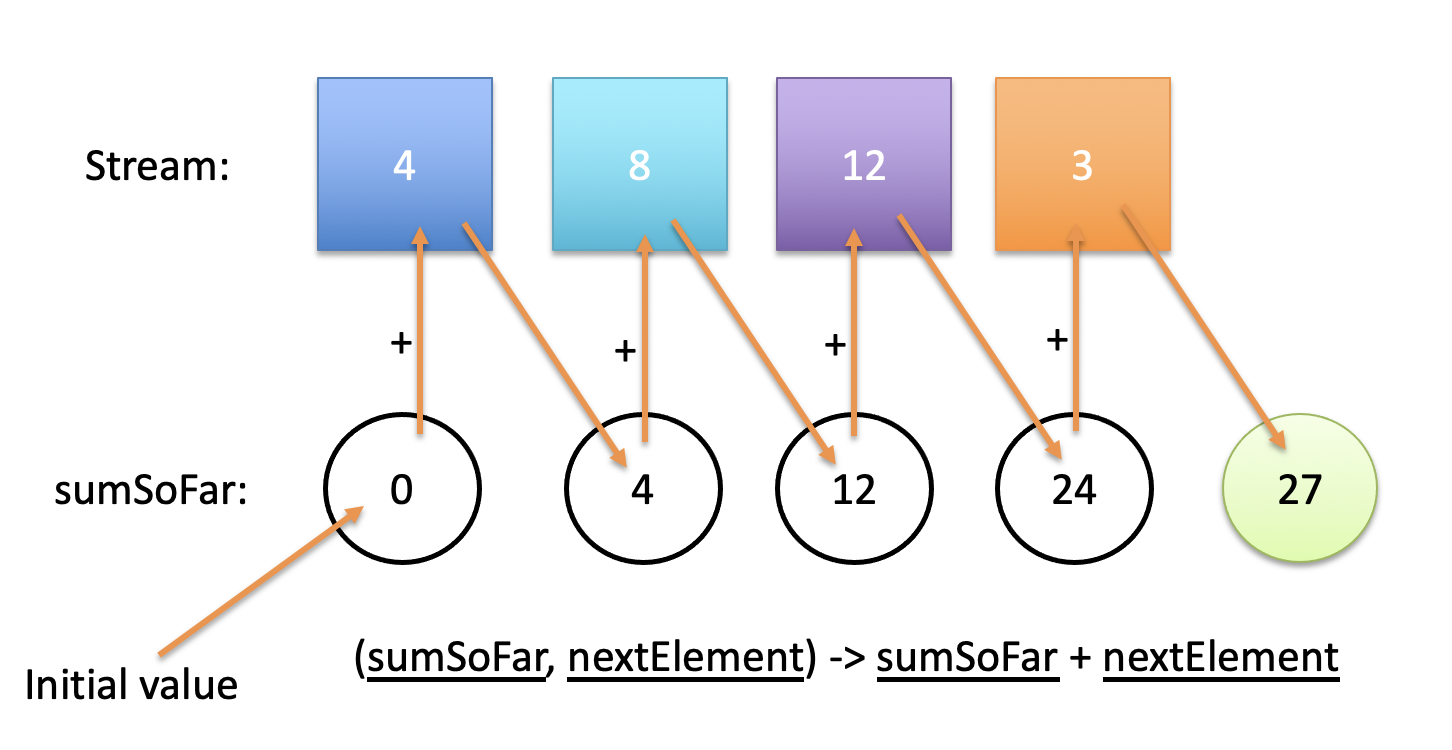
\includegraphics[width=\linewidth]{images/h6/stream_reduce.png}}
\caption{Reduce in actie}
\label{fig:stream_reduce}
\end{figure}

\subsection{Intermediate operation .flatMap()}

De intermediate operation flatMap wordt gebruikt om een Stream van verzamelingen te transformeren naar een stream van objecten. De elementen uit de verschillende verzameling worden bewerkt (map) en dan gecombineerd in 1 stream (flatten).

\begin{lstlisting}
List<String> animals = Arrays.asList("zebra", "dog", "dolphine");
List<String> names = Arrays.asList("Wannes", "Hans");
List<String> cities = Arrays.asList("Amsterdam", "Kopenhagen", "Oslo");
List<Integer> lengths = Stream.of(animals, names, cities)
		    .flatMap(l -> l.stream().map(String::length))
		    .collect(Collectors.toList());

assertEquals(Arrays.asList(5, 3, 8, 6, 4, 9, 10, 4), lengths);
\end{lstlisting}

\begin{figure}[H]
\frame{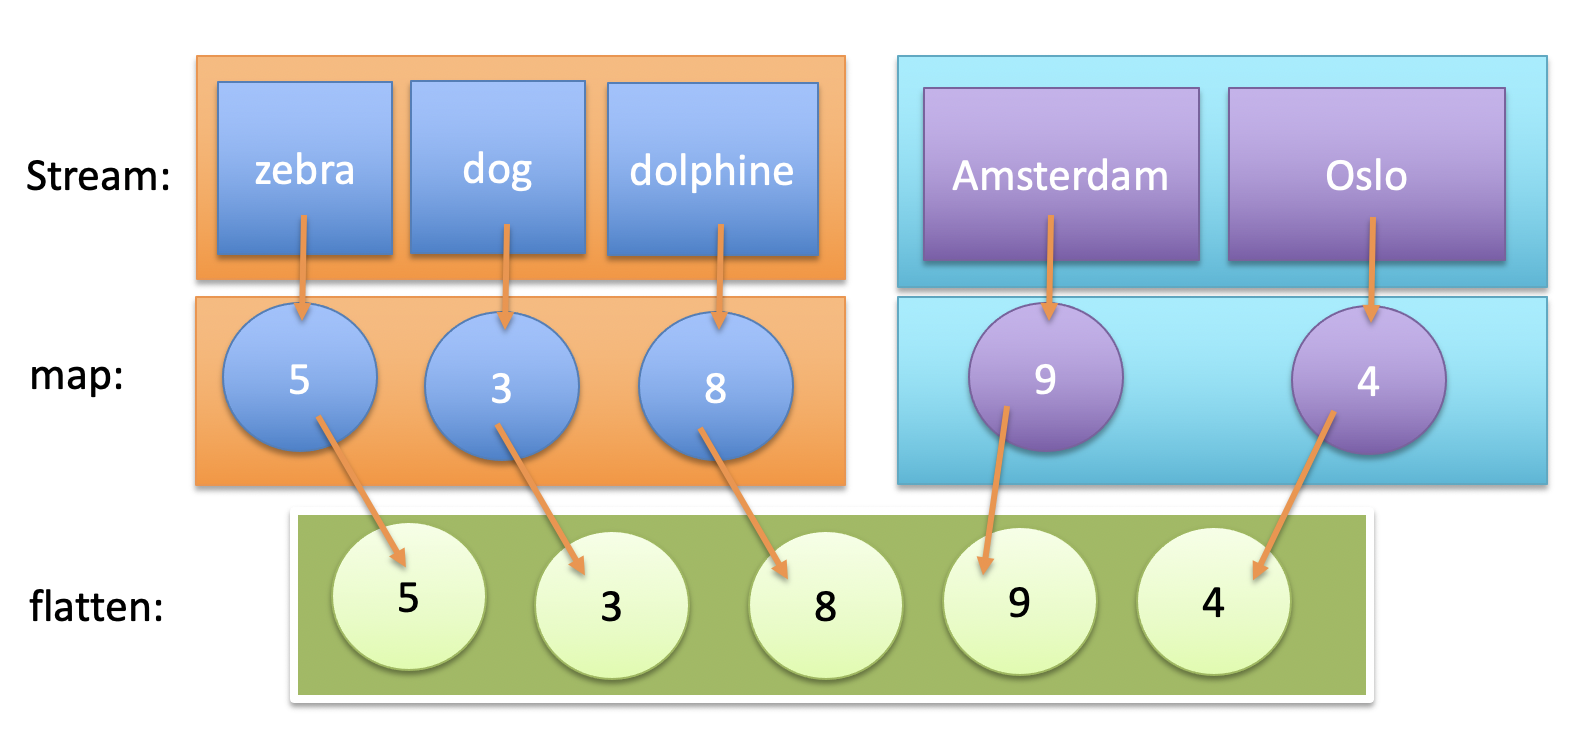
\includegraphics[width=\linewidth]{images/h6/stream_flatmap.png}}
\caption{flatMap in actie}
\label{fig:stream_flatmap}
\end{figure}

\section{Oefeningen}

\begin{oefening}

In de klasse be.pxl.ja.oefening1.StudentDao vind je een static methode createStudents(). Voorzie nu een hoofdprogramma waarin je start met deze lijst en de volgende vragen beantwoord met behulp van een stream.

\begin{itemize}
\item Welke studenten zijn er vandaag jarig. Toon hun naam. Je verandert best een geboortedata van de studenten om je stream uit te testen.
\item Toon alle gegevens van de student met de naam Carol.
\item Hoeveel studenten studeerden af in 2017?
\item Wat is de hoogste score ooit behaald? Wie behaalde deze hoogste score ooit?
\item Wie is de oudste persoon in de lijst?
\item Geef de namen van alle studenten gescheiden door komma (,) in  \'e\'en String.
\item Wie is de jongste student van afstudeerjaar 2018?
\item Maak een map met per afstudeerjaar de gemiddelde score.
\item Sorteer de studenten eerst op afstudeerjaar (recentste jaar eerst) en per afstudeerjaar volgens hun score (van hoog naar laag). Toon naam, afstudeerjaar en score.
\end{itemize}
\end{oefening}

\begin{oefening}

Bij een online kledingwinkel worden kortingen toegekend op de items in het winkelmandje. 
Het winkelmandje is een List van CartItem-objecten. Ieder gekocht item heeft een naam (bijv. "shoes", "hat", "dress",...) en een prijs (BigDecimal).
De items in het winkelmandje moeten niet uniek zijn, je kan bijvoorbeeld meerdere hoeden kopen. 

Maak een methode checkout die een winkemandje (List$<$CartItem$>$) als parameter aanneemt en de totale prijs van het winkelmandje berekent (return-type BigDecimal). Er worden dus kortingen toegekend. Indien je voor meer dan €100.0 aan schoenen (items met name ``shoes'') koopt, krijg je 20\% korting op het totaalbedrag van de schoenen.
Wanneer je minstens 2 hoeden koopt (items met name ``hat'') en voor een bedrag van minstens €50.0 dan krijg je €10.0 korting. Alle berekeningen schrijf je met behulp van streams.

Schrijf unit testen om de methode checkout grondig te testen.
\end{oefening}


\begin{oefening}

Maak een List waarvan de elementen opnieuw List-objecten zijn. Maak een methode sumLargest() die van iedere sublijst het hoogste getal neemt en deze getallen optelt. Maak hiervoor gebruik van streams.

Voor de volgende lijst:
\begin{verbatim}
 [list: [list: 1, 7, 5, 3], [list: 20], [list: 6, 9]]
\end{verbatim}
krijg je als resultaat 36 (7 + 20 + 9).

Je mag ervan uitgaan dat iedere sublijst elementen bevat. 

Schrijf unittesten voor de methode sumLargest().
 \end{oefening}
 
 
 \chapter{Java I/O}
 
 \begin{summary}
 Input en output, I/O in het kort, is een belangrijk onderdeel van een programmeertaal. 
 In dit hoofdstuk gaan we aan de slag met bestanden op een bestandssysteem.
 \end{summary}
 
 \section{Toegang tot bestanden en directories}
 
Een bestandsysteem bevat een verzameling van directories of mappen. Iedere directory bevat vervolgens subdirectories en eventueel bestanden.

Het pad naar een bestand, vanaf de root bekeken, is afhankelijk van het besturingssysteem.

\begin{table}[h!]
\centering
\begin{tabularx}{\textwidth}{| l | X |}
 \hline
 Besturingssysteem & Absoluut pad\\ 
 \hline
 Mac OS X & /Users/mark/courses/JavaAdvanced/Car.java \\
 Windows & C:\textbackslash public\textbackslash html\textbackslash javafaq\textbackslash index.html\\
 Unix & /home/mark/courses/slides.pdf \\
 \hline
 \end{tabularx}
 \end{table}
 
Java is platformonafhankelijk. De code om een bestand te lezen op Mac OS X zal dus identiek zijn als op Windows of Unix. Je maakt als ontwikkelaar gebruik van platformonafhankelijke interfaces. De achterliggende implementatie is afgeschermd voor de ontwikkelaar.
 
Laat ons eerst eens kijken naar het scheidingsteken dat we gebruiken om het pad op te bouwen.
Dit scheidingsteken kunnen we opvragen door systeemeigenschappen te gebruiken.  Naast de systeemeigenschap (system property) ``file.separator'' zijn er nog enkele handige waarden die je in je programma kan gebruiken.

\begin{lstlisting}
package be.pxl.ja;

public class Demo01 {

	public static final String SEPARATOR = System.getProperty("file.separator");

	public static void main(String[] args) {
		System.out.println("Current operating system: " + System.getProperty("os.name"));
		System.out.println("File separator: " + SEPARATOR);
		System.out.println("User's home directory: " + System.getProperty("user.home"));
		System.out.println("Current working directory: " + System.getProperty("user.dir"));
	}
}
\end{lstlisting}

Wanneer je dit programma uitvoert op Mac OS X krijg je bijvoorbeeld de volgende output:
\begin{verbatim}
Current operating system: Mac OS X
File separator: /
User's home directory: /Users/mark
Current working directory: /Users/mark/PXL/JavaAdv/JavaIO
\end{verbatim}

En op het Windows besturingssysteem:
\begin{verbatim}
Current operating system: Windows 10
File separator: \
User's home directory: C:\Users\20003575
Current working directory: C:\Users\20003575\Documents\PXL\JavaAdv\JavaIO
\end{verbatim}

Maar nu terug naar onze initi\"ele vraag: Hoe kunnen we het pad naar een directory of bestand samenstellen?

Absolute paden zijn afhankelijk van het besturingssysteem en kunnen dus bugs en problemen veroorzaken. Je moet dus hardgecodeerde, absolute paden vermijden in je programma's. Best stel je paden at runtime samen door gebruik te maken van systeemeigenschappen en input van de gebruiker.

We bestuderen in dit hoofdstuk interfaces en klassen uit \textit{java.io} en \textit{java.nio}. 
We gaan klassen uit de originele \textit{java.io} library gebruiken om bestanden te lezen en te schrijven. De nieuwere library \textit{java.nio} biedt ons een aantal klassen die het werken met bestanden eenvoudiger maken. \textit{nio} staat voor non-blocking IO. Deze non-blocking manier om bestanden te lezen en te schrijven valt buiten de scope van deze cursus.

Starten doen we met een aantal klassen uit het package \textit{java.nio.file}.

\begin{itemize}
\item De klasse \textbf{FileSystem}: stelt het onderliggend bestandssysteem voor en zorgt ervoor dat er Path-objecten gemaakt kunnen worden.
\item De interface \textbf{Path}: wordt gebruikt om een bestand of directory in een bestandssysteem te localiseren.
\item De klasse \textbf{Files}: deze klasse voorziet static methoden om bewerkingen met bestanden en directories uit te voeren.
\end{itemize}

\subsection{De klasse FileSystem en de interface Path}

Een Path-object cre\"eer je door de static methode \textit{of} van de interface Path aan te roepen. 

\begin{figure}[H]
  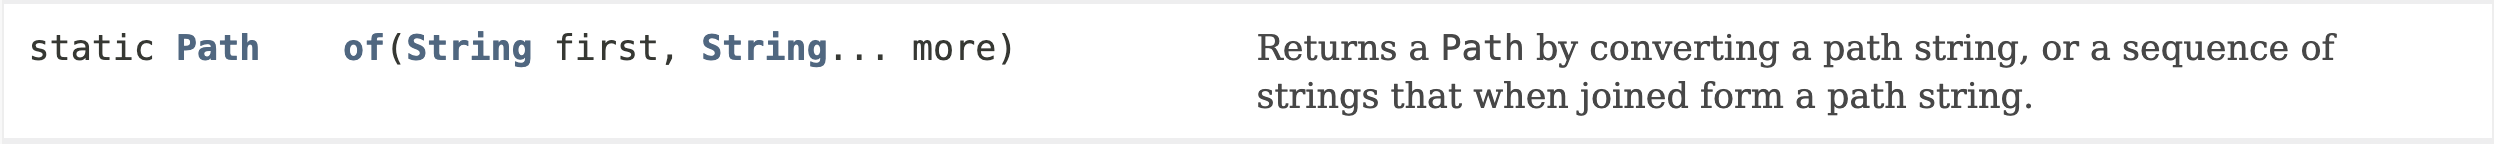
\includegraphics[width=\linewidth]{images/h8/path_of.png}
  \caption{Static methode of in de interface Path}
  \label{fig:paths}
\end{figure}

Achterliggend zal een object van de klasse FileSystem gebruikt worden om Path-objecten te cre\"eeren. FileSystem is wat we noemen een ``factory'' voor Path-objecten. De concrete klasse van een aangemaakt Path-object is afhankelijk van het besturingssysteem.

\begin{lstlisting}
import java.nio.file.FileSystem;
import java.nio.file.FileSystems;
import java.nio.file.Files;
import java.nio.file.Path;

public class Demo02 {

	public static void main(String[] args) {
		FileSystem defaultFileSystem = FileSystems.getDefault();
		System.out.println(defaultFileSystem.getClass());
		for (Path rootDirs: defaultFileSystem.getRootDirectories()) {
			System.out.println(rootDirs);
		}
		Path srcDir = Path.of(System.getProperty("user.dir"), "src");
		System.out.println(srcDir.toAbsolutePath());
		System.out.println(srcDir.getClass().getName());
		System.out.println(Files.isDirectory(srcDir));
	}

}
\end{lstlisting}

Bovenstaand programma geeft volgende uitvoer op een Mac OS X besturingssysteem.

\begin{verbatim}
class sun.nio.fs.MacOSXFileSystem
/
/Users/mark/PXL/JavaAdv/JavaIO/src
sun.nio.fs.UnixPath
true
\end{verbatim}

Volgende uitvoer zal er verschijnen als je het programma uitvoert op een Windows besturingssysteem.

\begin{verbatim}
class sun.nio.fs.WindowsFileSystem
C:\
D:\
C:\Users\20003575\Documents\PXL\JavaAdv\JavaIO\src
sun.nio.fs.WindowsPath
true
\end{verbatim}


\begin{oefening}
Maak via Windows verkenner (of Finder op Mac OS X) de volgende bestandsstructuur aan in directory waarnaar verwezen wordt door de systeemeigenschap \textit{user.home}.

\begin{figure}[H]
  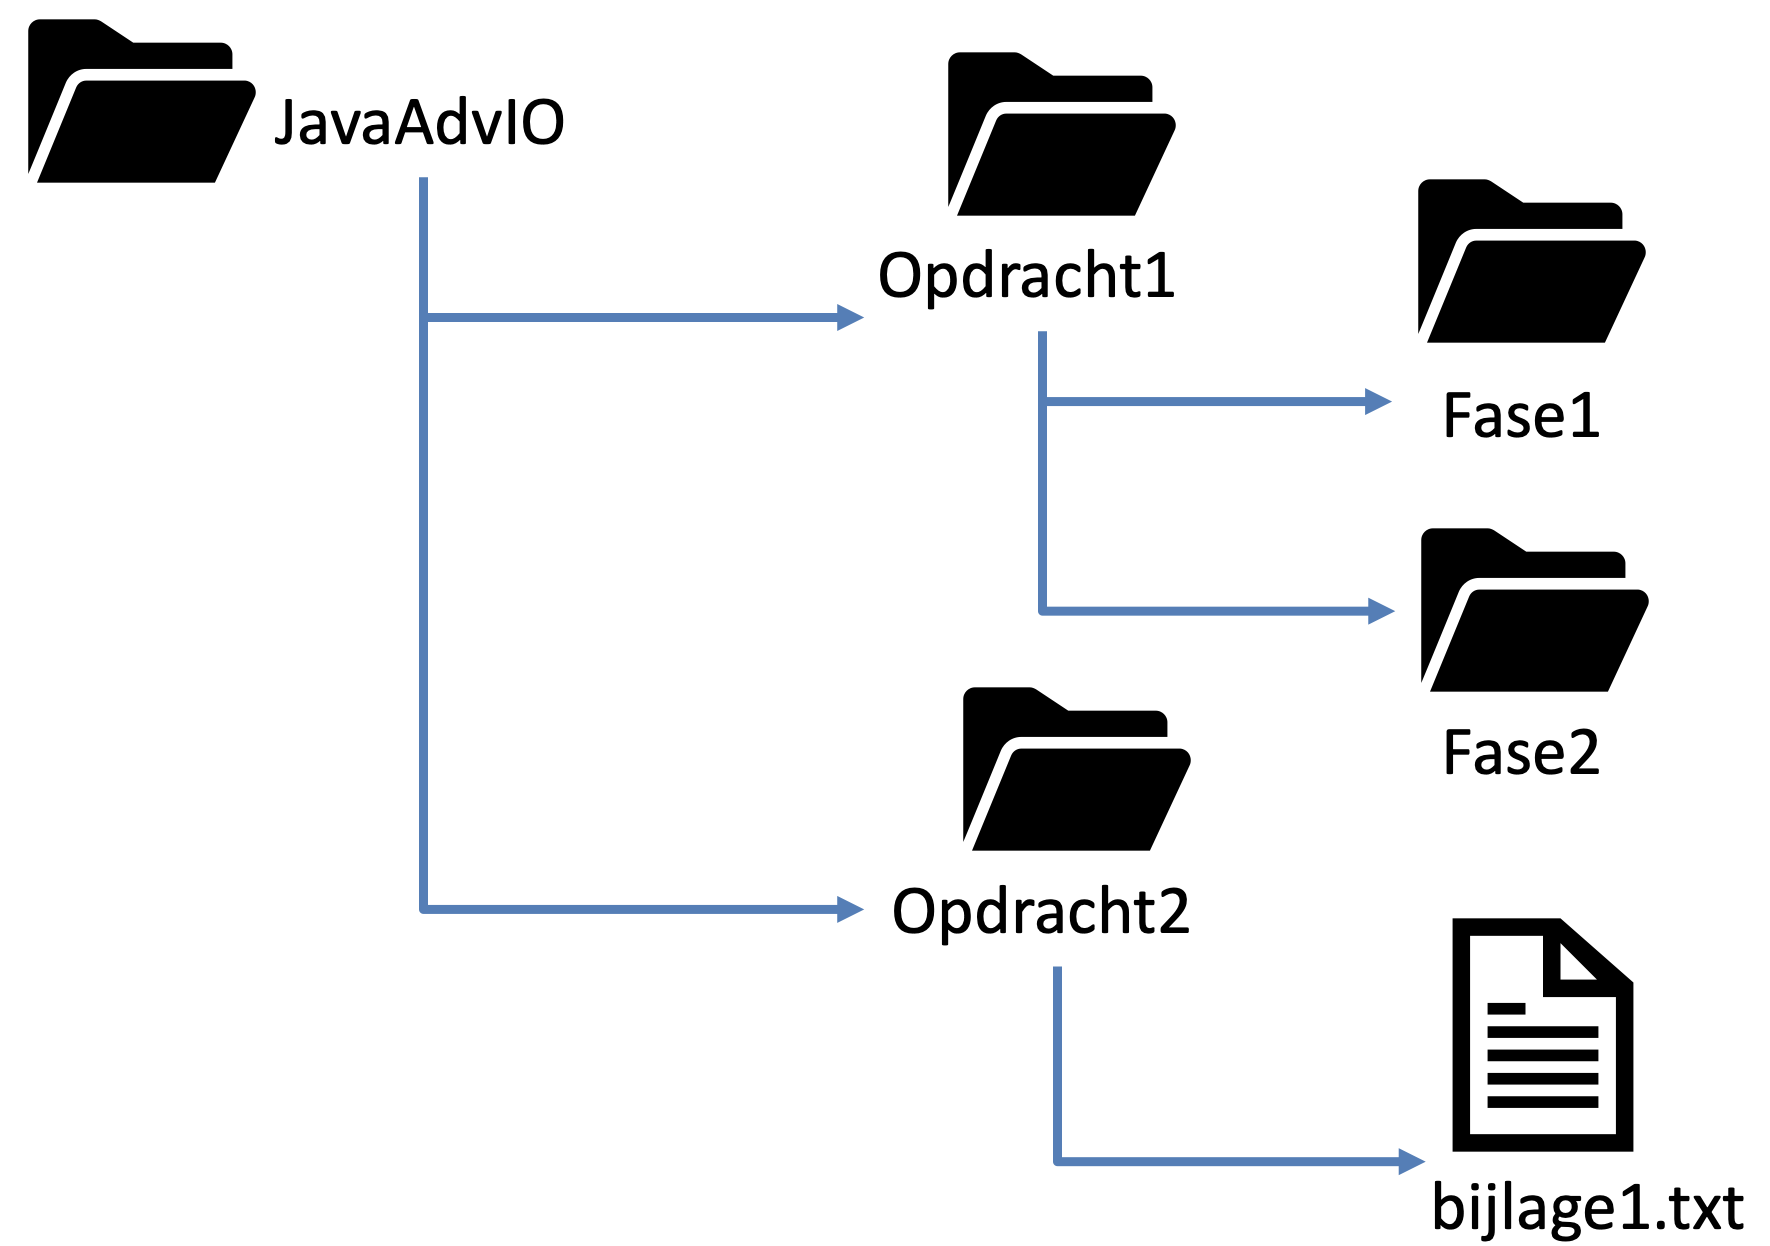
\includegraphics[width=\linewidth]{images/h8/opgave1.png}
  \caption{Bestandsstructuur}
  \label{fig:paths}
\end{figure}

\begin{itemize}
\item Vorm de systeemeigenschap user.home om tot een Path-object.
\item Welke concrete klasse heeft dit Path object?
\item Gebruik de methode resolve() van het Path object, om vanuit de directory user.home het path ``JavaAdvIO/Opdracht1/Fase2'' te volgen.
\item Wat is het resultaat wanneer je volgende methoden uitvoert op het laatst geconstrueerde Path?
\subitem toString()
\subitem getFileName()
\subitem getName(0)
\subitem getNameCount()
\subitem subpath(0,2)
\subitem getParent()
\subitem getRoot()
\end{itemize}
\end{oefening}

\subsection{Het factory ontwerppatroon}

Ontwerppatronen of design patterns zijn bepaalde structuren van klassen en interfaces die veelvoorkomende ontwerpproblemen bij het bouwen van software oplossen.

In de github repository vind je een eenvoudig voorbeeld van het factory ontwerppatroon in het package \textit{be.pxl.ja.factory}.
Veronderstel dat je een software-systeem bouwt waarbij je naar de gebruikers berichten stuurt. De gebruiker kan kiezen of hij de berichten per SMS of per email wil ontvangen. 


\subsection{De utility klasse Files}

De utility klasse \textit{java.nio.files.Files} bezit een groot aantal static methoden om bewerkingen met directories en bestanden uit te voeren.

\begin{oefening}
Zoek de documentatie van de klasse java.nio.files.Files op.
\end{oefening}

\subsubsection{Directories en bestanden aanmaken}

De static methode \textit{createDirectory} kan je gebruiken om een nieuwe directory aan te maken. 


\begin{lstlisting}
import java.io.IOException;
import java.nio.file.Files;
import java.nio.file.Path;

public class Demo03CreatingDirectoriesAndFiles {

	public static void main(String[] args) {
		Path path = Path.of(System.getProperty("user.home"), "JavaAdvIO", "Opdracht3", "bijlage.txt");
		if (Files.notExists(path.getParent())) {
			try {
				Files.createDirectory(path.getParent());
			} catch (IOException e) {
				System.out.println("An error occured while creating directory " + path.getParent());
			}
		}
		if (Files.notExists(path)) {
			try {
				Files.createFile(path);
			} catch (IOException e) {
				System.out.println("An error occured while creating file " + path);
			}
		}
	}

}
\end{lstlisting}

\begin{oefening}
Neem de documentatie er eens bij. Welke exceptions kunnen zich voordoen? Welke van deze exceptions zijn checked? Welke unchecked?
\end{oefening}


\subsubsection{Bestanden lezen (kleine bestanden)}

Als je tekstbestanden met een beperkt aantal regels wil lezen kan je de static methode readAllLines gebruiken.

\begin{lstlisting}
import java.nio.file.Path;
import java.nio.file.Paths;
import java.util.List;
import java.util.Random;

public class Demo04ReadingFiles {
	private static final Random RANDOM = new Random();

	public static void main(String[] args) {
		Path path = Paths.get("resources/small_file_with_text.txt");

		try {
			List<String> text = Files.readAllLines(path);
			System.out.println(text.get(RANDOM.nextInt(text.size())));
		} catch (IOException e) {
			e.printStackTrace();
		}
	}
}
\end{lstlisting}

\subsubsection{Bestanden kopi\"eren}

Je kan eenvoudig bestanden kopi\"eren door gebruik te maken van de static methode copy.

\begin{lstlisting}
import java.io.IOException;
import java.nio.file.Files;
import java.nio.file.Path;
import java.nio.file.Paths;

public class Demo05CopyFiles {

	public static void main(String[] args) {
		Path original = Paths.get("resources/small_file_with_text.txt");
		Path copy = Paths.get("resources", "copy_" + System.currentTimeMillis() + ".txt");
		System.out.println(Files.exists(copy));
		try {
			Files.copy(original, copy);
			System.out.println(Files.exists(copy));
		} catch (IOException e) {
			e.printStackTrace();
		}
	}
}
\end{lstlisting}

\section{Tekstbestanden}

\subsection{I/O Streams}

Een I/O stream is een opeenvolging van bytes (8 bits). Je mag I/O streams zeker niet verwarren met de Stream API die we in het vorige hoofdstuk hebben besproken. InputStreams worden gebruikt om gegevens byte per byte aan te bieden aan een Java programma. OutputStreams worden gebruikt om gegevens vanuit een Java programma byte per byte te versturen naar een externe bron (dit kan een bestand zijn, maar ook een andere computer). 
In dit hoofdstuk zijn het bestanden die we als bron of doel van onze I/O streams gebruiken. Je kan tekstbestanden byte per byte gaan inlezen en wegschrijven, maar dit is niet effici\"ent. Karakters worden meestal voorgesteld door meerdere bytes. 
De karakter encodering bepaalt hoeveel bytes er per karakter gebruikt zullen worden. Bij UTF-8 bijvoorbeeld worden 1 tot 4 bytes gebruikt om de karakters voor te stellen. Een alternatief is dus dat je tekstbestanden karakter per karakter gaat inlezen, maar ook dit is niet altiijd effici\"ent.

\subsection{BufferedReader}

De klasse BufferedReader biedt een eenvoudige en effici\"ente manier om grotere tekstbestanden te lezen. Het groepeert (buffert) karakters uit een bestand zodat je het bestand regel per regel kan inlezen. De methode newBufferedReader uit de klasse Files vereenvoudigt het aanmaken van de BufferedReader voor ons.
Het einde van het tekstbestand is bereikt als readLine() \textit{null} geeft.

\begin{figure}[H]
  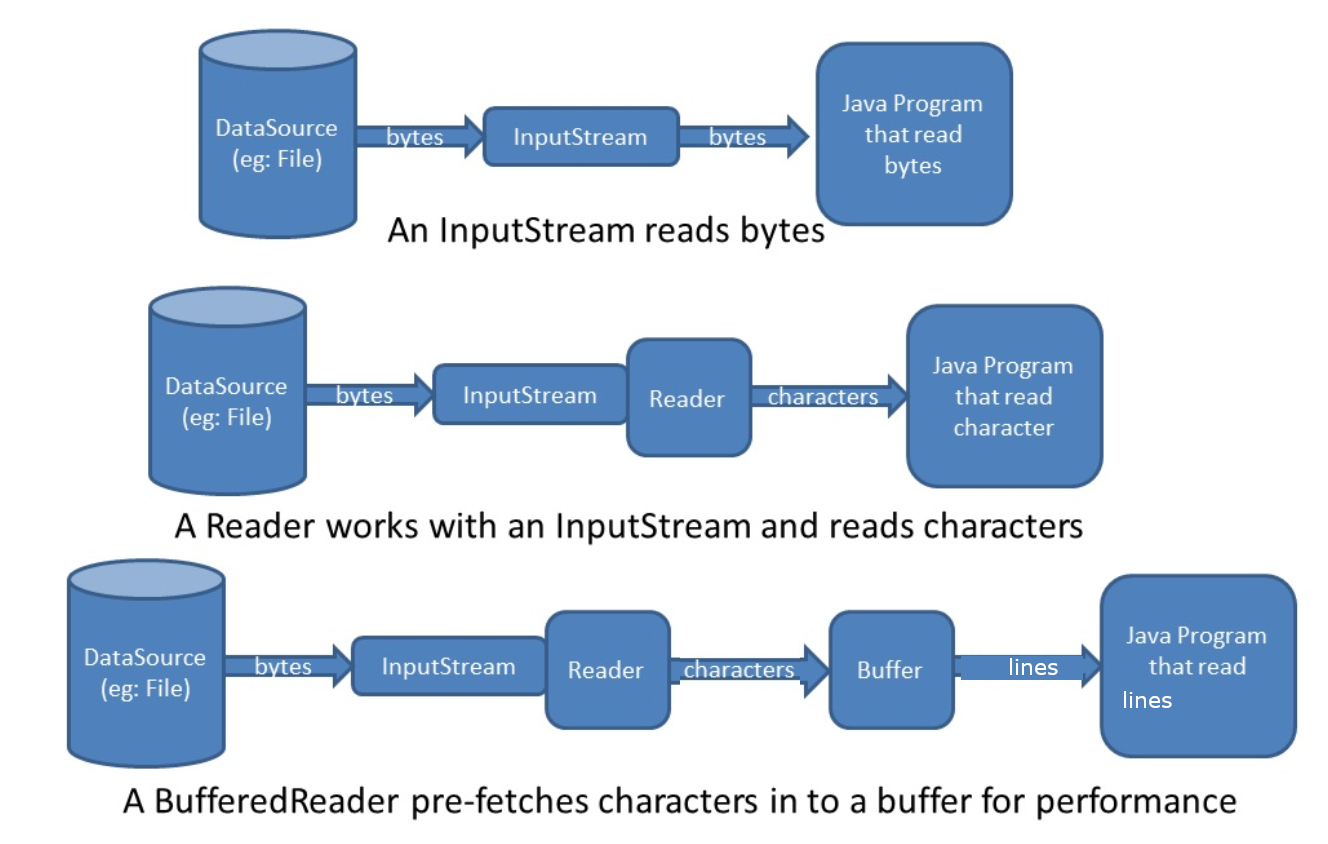
\includegraphics[width=\linewidth]{images/h8/stream_reader.png}
  \caption{InputStream, InputStreamReader en BufferedReader}
  \label{fig:paths}
\end{figure}

\begin{lstlisting}
import java.io.BufferedReader;
import java.io.IOException;
import java.nio.file.Files;
import java.nio.file.Paths;

public class Demo06BufferedReader {

	public static void main(String[] args) {

		try (BufferedReader reader =  Files.newBufferedReader(Paths.get("resources/small_file_with_text.txt"))) {
			String line = null;
			while ((line = reader.readLine()) != null) {
				System.out.println(line);
			}
		} catch (IOException e) {
			e.printStackTrace();
		}
	}
}
\end{lstlisting}

We maken in dit code-voorbeeld gebruik van \textbf{try-with-resources}.
De BufferedReader implementeert namelijk de interface \textit{java.lang.AutoCloseable}. Wanneer je klaar ben met het lezen of schrijven van een bestand, moet je dit namelijk aan het besturingssysteem laten weten. Het besturingssyteem zorgt ervoor dat de toegang tot een bestand goed beheerd wordt zodat er zich geen problemen voordoen wanneer er verschillende programma's gelijktijdig in hetzelfde bestand willen lezen en/of schrijven. Het sluiten van een bestand werd typisch ge\"implementeerd in een \textit{finally-block}. Tegenwoordig zijn veel resources (zoals bestanden) auto-closeable waardoor je deze code niet meer zelf moet schrijven. Door gebruik te maken van try-with-resources wordt het bestand automatisch netjes gesloten zodra het programma klaar is met het lezen of schrijven van het bestand.

\subsection{BufferedWriter}

In plaats van karakter per karakter in een bestand weg te schrijven, gaat BufferedWriter grotere stukken tekst in \'e\'en keer in het bestand wegschrijven. 


\begin{lstlisting}
import java.io.BufferedWriter;
import java.io.IOException;
import java.nio.file.Files;
import java.nio.file.Paths;
import java.util.Random;

public class Demo07BufferedWriter {

	private static final Random RANDOM = new Random();

	public static void main(String[] args) {

		int numberOfBugs = 99;

		try (BufferedWriter writer =  Files.newBufferedWriter(Paths.get("resources/poem.txt"))) {
			for (int i =0; i < 5; i++) {
				writer.write(numberOfBugs + " little bugs in the code,\n");
				writer.write(numberOfBugs + " little bugs in the code.\n");
				writer.write("Take one down, patch it around,\n");
				numberOfBugs += RANDOM.nextInt(50) ;
				writer.write(numberOfBugs + " little bugs in the code.\n");
				writer.newLine();
			}
		} catch (IOException e) {
			e.printStackTrace();
		}
	}

}
\end{lstlisting}

Nadat het programma is uitgevoerd bevat het bestand poem.txt.

\begin{verbatim}
99 little bugs in the code,
99 little bugs in the code.
Take one down, patch it around,
124 little bugs in the code.

124 little bugs in the code,
124 little bugs in the code.
Take one down, patch it around,
172 little bugs in the code.
...
\end{verbatim}

\subsection{Character sets}

\begin{lstlisting}
import java.nio.charset.Charset;

public class Demo7DefaultCharset {

	public static void main(String[] args) {

		System.out.println(Charset.defaultCharset().displayName());
	}

}
\end{lstlisting}

Met het bovenstaande programma kan je afdrukken wat de default encoding is die gebruikt wordt om bytes te combineren tot karakters. UTF-8 is de meest gebruikte encoding, maar toch is het een goede gewoonte om de gebruikte karakterset mee te geven als parameter wanneer je een bestand leest of schrijft. Op die manier kan je problemen vermijden.

\begin{lstlisting}
Files.newBufferedWriter(Paths.get("resources/myfile.txt"), Charset.forName("UTF-8"));
\end{lstlisting}

\subsection{Het decorator patroon}

De BufferedReader heeft als basis een InputStreamReader waaraan extra functionaliteit wordt toegevoegd, namelijk het bufferen van de karakters. De InputStreamReader vormt op zijn beurt de brug tussen byte streams en character streams. Hij leest bytes en decodeert ze tot karakters door gebruik te maken van een karakterset (Charset).

Wat we bij deze klassen is dat ze ontwikkeld zijn volgens het decorator ontwerppatroon.
In het package \textit{be.pxl.ja.decorator} vind je een eenvoudig voorbeeld van dit ontwerppatroon.

\section{Programma attributen}

Het is een goed idee om Java programma's gemakkelijk configureerbaar te maken. 
Om dit te verwezenlijken zijn parameters bestaande uit een key en een value meestal voldoende. 
In Java gebruik je de klasse \textit{java.util.Properties} om configuratie-bestanden te lezen en weg te schrijven.
Je gebruikt de methode load om een configuratie-bestand in te lezen en store om de eigenschappen weg te schrijven. Met de methode getProperty kan je aan de hand van een key de bijhorende waarde opvragen.

\begin{lstlisting}
import java.io.IOException;
import java.io.InputStream;
import java.io.OutputStream;
import java.nio.file.Files;
import java.nio.file.Path;
import java.util.Properties;
import java.util.Scanner;

public class Demo08ProgramWithProperties {
	private static final String CONFIG_FILE = "resources/config.properties";

	public static void main(String[] args) {
		try(InputStream inputStream = Files.newInputStream(Path.of(CONFIG_FILE))) {
			Properties properties = new Properties();
			properties.load(inputStream);
			System.out.println("Welcome " + properties.getProperty("demo.name") + "!");
			System.out.println("You're mails will be sent to: " + properties.getProperty("demo.email"));
		} catch (IOException e) {
			createProperties();
		}
	}

	private static void createProperties() {
		Scanner scanner = new Scanner(System.in);
		System.out.println("You're using this program for the first time.");
		System.out.println("What's your name:");
		String name = scanner.nextLine();
		System.out.println("What's your company:");
		String company = scanner.nextLine();
		System.out.println("What's your email:");
		String email = scanner.nextLine();
		Properties properties = new Properties();
		properties.setProperty("demo.name", name);
		properties.setProperty("demo.company", company);
		properties.setProperty("demo.email", email);
		try(OutputStream outputStream = Files.newOutputStream(Path.of(CONFIG_FILE))) {
			properties.store(outputStream, "Demo program configuration");
		}
		catch (IOException e) {
			System.out.println("We were not able to save your configuration.");
		}
	}
}
\end{lstlisting}

De eerste keer dat het programma wordt uitgevoerd, is het bestand config.properties bestand nog niet aanwezig is. De gebruiker wordt dan gevraagd om zijn gegevens in te voeren.

\begin{verbatim}
You're using this program for the first time.
What's your name:
Nele
What's your company:
PXL
What's your email:
nele.custers@pxl.be
\end{verbatim}

Je zal zien dat er na het uitvoeren van het programma een bestand \textit{resources/config.properties} is aangemaakt.
Dit bestand bevat de volgende informatie.

\begin{verbatim}
#Demo program configuration
#Tue Nov 17 09:13:51 CET 2020
demo.name=Nele
demo.company=PXL
demo.email=nele.custers@pxl.be
\end{verbatim}
Wanneer je het programma opnieuw opstart, wordt het .properties bestand gelezen en krijg je de volgende output.

\begin{verbatim}
Welcome Nele!
You're mails will be sent to: nele.custers@pxl.be
\end{verbatim}


\section{Byte stream}

Object serialization laat ons toe om de status (de waarden van de eigenschappen) van een object te converteren naar een byte stream. Op die manier kan een object weggeschreven worden in bestand of verstuurd worden over een netwerk.
Deserialization is het omgekeerde proces, waarbij de byte stream terug wordt geconverteerd naar een object.

Enkel objecten van klassen die de interface \textit{Serializable} implementeren kunnen geserialiseerd worden.
Je kan een eigenschap van een klasse \textbf{transient} maken als je de waarde van die eigenschap niet wil serialiseren.

Alle static eigenschappen behoren tot de klasse en niet tot een object, dus de waarden van static field kunnen nooit geserialiseerd worden. 

De klasse ObjectOutputStream die we gebruiken om objecten te schrijven en de klasse ObjectInputStream die we gebruiken om objecten in te lezen, zijn opnieuw implementaties van het decorator patroon. We gaan respectievelijk de klassen FileOutputStream en FileInputStream ``decoreren'' met extra functionaliteit om te werken met volledige objecten in plaats van bytes. 

\subsection{Object serialization}

\begin{lstlisting}
import java.io.FileOutputStream;
import java.io.IOException;
import java.io.ObjectOutputStream;
import java.time.LocalDate;
import java.util.Arrays;
import java.util.List;

public class Demo09Serialization {

	public static void main(String[] args) {
		Student student = new Student("Mare", LocalDate.of(2000, 11, 29));
		student.setGraduationDate(LocalDate.of(2018, 6, 30));
		List<String> animals = Arrays.asList("elephant", "zebra", "donkey");
		try (FileOutputStream file = new FileOutputStream("resources/demo.ser");
		     ObjectOutputStream out = new ObjectOutputStream(file)) {
			out.writeObject(student);
			out.writeObject(animals);
		} catch (IOException ex) {
			System.out.println(ex.getMessage());
		}
	}
}
\end{lstlisting}


\subsection{Object deserialization}

\begin{lstlisting}
import java.io.FileInputStream;
import java.io.IOException;
import java.io.ObjectInputStream;
import java.util.List;

public class Demo09Deserialization {

	public static void main(String[] args) {
		try (FileInputStream file = new FileInputStream("resources/demo.ser");
		     ObjectInputStream in = new ObjectInputStream(file)) {
			Student student = (Student) in.readObject();
			System.out.println(student.getName());
			System.out.println(student.getDateOfBirth());
			List<?> animals = (List<?>) in.readObject();
			//List<String> animals = (List<String>) in.readObject();
			System.out.println(animals.size());
			System.out.println(animals.get(0));
		} catch (IOException ex) {
			System.out.println(ex.getMessage());
		} catch (ClassNotFoundException e) {
			e.printStackTrace();
		}
	}
}
\end{lstlisting}


%\subsection{Audio en afbeeldingen}



\section{Oefeningen}

\begin{oefening}
\textbf{Telefoonboek}\\

Schrijf een programma om telefoonnummers bij te houden.
Wanneer je het programma opstart wordt het bestand phonedirectory.txt ingelezen,
plaats dit dus in een nieuwe folder (bv. resources) in je project. Iedere lijn in het
bestand heeft het volgende formaat: $<naam>;<tel1>;<tel2>;…$
We geven alvast wat startcode voor het printen van het menu.
(PhoneNumbersApp.java)
\begin{itemize}
\item Lees alle lijnen in en steek alle contacten in een Collection, zodat je aan de hand van
een naam de bijhorende telefoonnummers kan zoeken. Let op: er kunnen meerdere
telefoonnummers aan één contact gelinkt worden.
\item Zorg ook voor functionaliteit om telefoongegevens toe te voegen (zie reeds gegeven
code). Als je een telefoonnummer toevoegt dat reeds bestaat voor de gegeven
persoon, gooit het programma een zelfgemaakte exception. (bv.
PhoneDirectoryException). Deze exception moet niet opgevangen worden, dus het
programma mag stoppen met uitvoeren in dit geval.
\item Wanneer je ervoor kiest om het programma af te sluiten, worden alle gegevens eerst
weer weggeschreven in phonedirectory.txt, zodat geen gegevens verloren gaan.
\end{itemize}
\end{oefening}

\begin{oefening}
\textbf{Bank account}\\

Schrijf een applicatie voor het beheren van spaarrekeningen.
Voorzie volgende functionaliteit:
\begin{itemize}
\item Maak een klasse Spaarrekening met de nodige member variabelen (bv. saldo,
naam, nummer, …)
\item Zorg dat instanties van deze klasse als object naar een file geschreven kunnen
worden (Serializable interface)
\item Schrijf in een main methode de code om een volledig Spaarrekening object
naar een file weg te schrijven.
\item Voeg code toe om een spaarrekening object terug uit te lezen uit deze file.
\item Controleer of de member variabelen hun waarde hebben behouden na uitlezen.
\end{itemize}
\end{oefening}


\chapter{Multithreading}

\begin{summary}
Multithreading is een belangrijk concept in Java. Er worden twee of meer delen van een programma tegelijkertijd uitgevoerd om zo de CPU zo maximaal mogelijk te benutten.
Computerspelletjes, computersimulaties, webservers, browsers,... zijn voorbeelden van programma's waarbij het gebruik van multithreading noodzakelijk is. Verschillende frameworks die dagelijks worden gebruikt door bedrijven die Java programma's ontwikkelen, maken onderliggend gebruik van multithreading. Het is daarom belangrijk om de basisconcepten te begrijpen.
\end{summary}

\section{Wat zijn threads?}

Om de term multithreading goed te begrijpen starten we met het verschil uit te leggen tussen een thread en een proces. Een proces is een programma dat wordt uitgevoerd.
Een process kan bestaan uit \'e\'en of meerdere uitvoeringspaden. Deze mini-processen binnen een proces noemen we threads. We spreken over multithreading als we een programma schrijven waarin er meerdere threads zijn ge\"implementeerd die tegelijkertijd uitgevoerd kunnen worden. 
De verschillende threads binnen een process kunnen tegelijkertijd uitgevoerd worden, zodat de CPU maximaal gebruikt worden. 
Bij een single-core CPU is er een scheduler die beslist welke thread wordt uitgevoerd en die context switching tussen de verschillende threads regelt. Deze context switching gebeurt zo snel dat het lijkt alsof er vanalles tegelijk gebeurt in het programma. Stel dat je pacman speelt op een single-core CPU. De spookjes verplaatsen zich voortdurend over het scherm en jij geeft ondertussen keyboard commando's om pacman te besturen en de spookjes te ontwijken.

Bij een multi-core CPU kan het uitvoeren van verschillende threads echt tegelijkertijd gebeuren. Toch zal er nog steeds een scheduler moeten waken dat alle threads een gelijk deel van de tijd aan de beurt komen.  

\begin{figure}[H]
  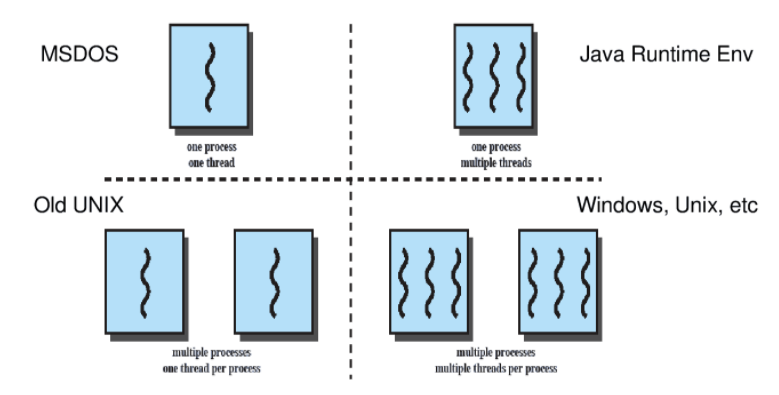
\includegraphics[width=\linewidth]{images/h9/process_threads.png} 
  \caption{Relatie tussen proces en threads}
  \label{fig:proces_thread}
\end{figure}

\begin{figure}[H]
  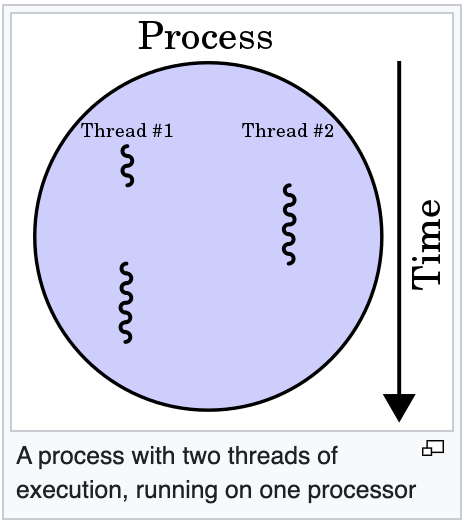
\includegraphics[scale=1]{images/h9/process_with_two_threads.png}
  \label{fig:proces_thread_2}
\end{figure}

Multitasking is de mogelijkheid om meer dan 1 taak op hetzelfde ogenblik uit voeren.
Java voorziet dus thread-based multitasking. Binnen een proces delen de threads een gedeelte van het geheugen. Dit gedeelte, de \textbf{heap}, is waar de objecten leven.
Iedere thread heeft ook een stukje priv\'e-geheugen dat gebruikt wordt tijdens het uitvoeren van de thread. Dit gedeelte van het geheugen noemen we de \textbf{stack}.
Als de scheduler beslist om een volgende thread binnen een proces aan het werk te zetten, gebeurt deze context-switch heel efficient.



\section{Threads zijn objecten}

Threads zijn objecten in Java. 
Alle Java programma's hebben minstens \'e\'en thread, de main thread, die aangemaakt wordt door de JVM (Java Virtual Machine) als het programma wordt gestart. De main()-method wordt uitgevoerd door de main thread. 
Daarnaast kan je extra threads aanmaken.
Je cre\"eert deze objecten
door een subklasse van de klassse Thread te maken of de functionele interface Runnable te implementeren. We bekijken beide mogelijkheden.

\subsection{Subklasse van Thread}

Wanneer je een subklasse maakt van de klasse Thread overschrijf je de run() methode. De run() methode bevat de instructies die de thread zal uitvoeren zodra je de methode start() aanroept.

\begin{lstlisting}
public class WorkerThread extends Thread {

	@Override
	public void run() {
		System.out.println("Line A (" + Thread.currentThread().getName() + ")");
		System.out.println("Line B (" + Thread.currentThread().getName() + ")");
		System.out.println("Line C (" + Thread.currentThread().getName() + ")");
		System.out.println("Line D (" + Thread.currentThread().getName() + ")");
		System.out.println("Line E (" + Thread.currentThread().getName() + ")");
	}

	public static void main(String[] args) {
		WorkerThread workerThread = new WorkerThread();
		workerThread.start();
		System.out.println("Line 1 (" + Thread.currentThread().getName() + ")");
		System.out.println("Line 2 (" + Thread.currentThread().getName() + ")");
		System.out.println("Line 3 (" + Thread.currentThread().getName() + ")");
	}
}
\end{lstlisting}

Zodra een instantie van de klasse WorkerThread is opgestart wisselt de scheduler tussen de main-thread en de instantie workerThread. Op een single-processor computer lijkt het of de threads gelijktijdig worden uitgevoerd, op een multi-processor kunnen de threads effectief gelijktijdig worden uitgevoerd.

Hier is een mogelijk verloop van het programma. 

\begin{verbatim}
Line A (Thread-0)
Line 1 (main)
Line B (Thread-0)
Line 2 (main)
Line C (Thread-0)
Line 3 (main)
Line D (Thread-0)
Line E (Thread-0)
\end{verbatim}

\subsection{De interface Runnable implementeren}

Een tweede manier om een thread te programmeren is door een klasse te cre\"eeren die de interface java.lang.Runnable implementeert. Ook hier voorzie je een implementatie van de run() methode. 
Om de thread te starten moet je een instantie van de klasse die de Runnable interface implementeert doorgeven als parameter aan een constructor van de klasse Thread. Vervolgens kan je de methode start() aanroepen.

\begin{lstlisting}
public class WorkerThread2 implements Runnable {

	@Override
	public void run() {
		System.out.println("Line A (" + Thread.currentThread().getName() + ")");
		System.out.println("Line B (" + Thread.currentThread().getName() + ")");
		System.out.println("Line C (" + Thread.currentThread().getName() + ")");
		System.out.println("Line D (" + Thread.currentThread().getName() + ")");
		System.out.println("Line E (" + Thread.currentThread().getName() + ")");
	}

	public static void main(String[] args) {
		WorkerThread2 workerThread = new WorkerThread2();
		new Thread(workerThread).start();
		System.out.println("Line 1 (" + Thread.currentThread().getName() + ")");
		System.out.println("Line 2 (" + Thread.currentThread().getName() + ")");
		System.out.println("Line 3 (" + Thread.currentThread().getName() + ")");
	}
}
\end{lstlisting}

Een vaakgeziene fout is dat de methode run() wordt aangeroepen in plaats van de methode start(). Op het eerste zicht zal dit geen probleem opleveren. Maar het is dan GEEN programma met multithreading. De main-thread gaat dan de instructies van de run() methode uitvoeren. Test het even uit door in het bovestaande programma het run() aan te roepen in plaats van start(). Zorg dus dat je deze fout niet maakt!

\subsubsection{Runnable als lambda expressie}

Omdat de interface Runnable een functionele interface is, kan je ook gebruikmaken van een lambda expressie.

\begin{lstlisting}
public class WorkerThread3 {

	public static void main(String[] args) {
		new Thread(() -> {
			System.out.println("Line A (" + Thread.currentThread().getName() + ")");
			System.out.println("Line B (" + Thread.currentThread().getName() + ")");
			System.out.println("Line C (" + Thread.currentThread().getName() + ")");
			System.out.println("Line D (" + Thread.currentThread().getName() + ")");
			System.out.println("Line E (" + Thread.currentThread().getName() + ")");
		}).start();
		System.out.println("Line 1 (" + Thread.currentThread().getName() + ")");
		System.out.println("Line 2 (" + Thread.currentThread().getName() + ")");
		System.out.println("Line 3 (" + Thread.currentThread().getName() + ")");
	}
}
\end{lstlisting}


\subsection{Thread class versus Runnable Interface}

Het kan een beetje verwarrend zijn dat je 2 mogelijkheden hebt om threads te implementeren. Er zijn echter belangrijke verschillen tussen beide implementaties. Wanneer je een subklasse maakt van Thread, dan zijn objecten van deze klasse ``echte'' thread objecten en heb je als ontwikkelaar volledige controle over de thread. Wanneer je de Runnable interface gebruikt, definieer je eigenlijk alleen het werk dat door de thread uitgevoerd moet worden. Je hebt dan geen controle over de thread zelf. 
Als je een subklasse van de klasse Thread maakt, kan je overigens geen tweede superklasse gebruiken omdat Java geen meervoudige overerving (multiple inheritance) toelaat. Als je dus toch van een andere superklasse wil overerven gebruik je de interface Runnable.

\section{Thread life cycle}

Een Java thread heeft altijd \'e\'en van de volgende statussen:
\begin{itemize}
\item NEW\\
Zodra je een Thread-object aanmaakt, heeft deze de status \textit{NEW}. Zodra de methode \textit{start()} wordt aangeroepen verandert de status van de thread van NEW naar RUNNABLE.
\item RUNNABLE\\
Een thread die wordt uitgevoerd in de JVM (Java Virtual Machine) bevindt zich in deze status. Er zijn 2 mogelijkheden: ofwel wordt de thread effectief uitgevoerd, ofwel is de thread klaar om uitgevoerd te worden, maar wacht hij even op een beschikbare processor.
\item BLOCKED\\
Een thread is in status BLOCKED wanneer de thread moet wachten om een gesynchroniseerd code-fragment uit te voeren. Een gesynchroniseerd code-fragment is een methode of een deel van een methode dat maar door 1 thread mag uitgevoerd worden. Als 1 thread deze code uitvoert, moeten de andere threads, die met dit code-fragment willen starten, wachten. We gaan in het onderdeel synchronisatie hier dieper op in. 
\item WAITING\\
Een thread is in de status WAITING als hij wacht op een andere thread die eerst een bepaalde actie moet uitvoeren.
\item TIMED\_WAITING\\
Een thread is in de status timed\_waiting als hij, net als bij de status waiting wacht op een andere thread die een bepaalde actie moet uitvoeren. Het verschil is echter dat de thread een timeout heeft voorzien en na de vooringestelde tijd toch zal verdergaan.
\item TERMINATED\\
Een thread die klaar is met zijn taak bevindt zich in de status TERMINATED.
\end{itemize}

\begin{figure}[H]
  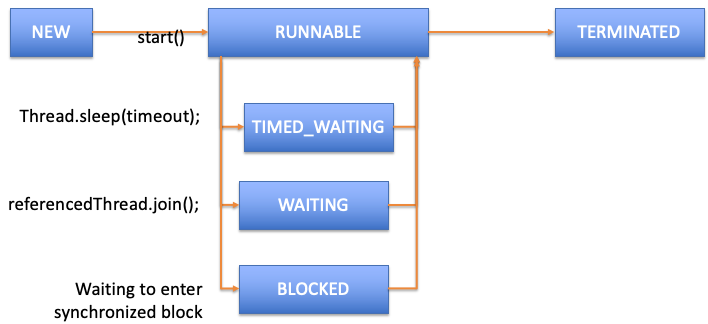
\includegraphics[width=\linewidth]{images/h9/thread_life_cycle.png}
  \label{fig:thread_life_cycle}
\end{figure}

\subsection{Thread.sleep()}

De methode Thread.sleep() kan gebruikt worden om een thread gedurende een bepaalde tijd (uitgedrukt in milliseconden) te pauzeren.
Let op dat deze methode een static methode is.
Wanneer de instructie Thread.sleep() wordt uitgevoerd zal de thread scheduler de aanroeper in WAIT status plaatsen voor de opgegeven tijd. Als deze tijd voorbij is, wordt de status van de thread terug RUNNABLE en daarna is het even wachten tot de CPU terug beschikbaar is om de uitvoer verder te zetten. De uiteindelijke tijd dat de thread dus zal ``slapen'' is dus afhankelijk van de thread scheduler.

\begin{lstlisting}
public class WorkerThreadWithSleep extends Thread {

	@Override
	public void run() {
		System.out.println("Line A (" + Thread.currentThread().getName() + ")");
		try {
			Thread.sleep(5000);
		} catch (InterruptedException e) {
			e.printStackTrace();
		}
		System.out.println("Line B (" + Thread.currentThread().getName() + ")");
		System.out.println("Line C (" + Thread.currentThread().getName() + ")");
		System.out.println("Line D (" + Thread.currentThread().getName() + ")");
		System.out.println("Line E (" + Thread.currentThread().getName() + ")");
	}

	public static void main(String[] args) {
		WorkerThreadWithSleep workerThread = new WorkerThreadWithSleep();
		System.out.println(workerThread.getState());
		workerThread.start();
		System.out.println(workerThread.getState());
		System.out.println("Line 1 (" + Thread.currentThread().getName() + ")");
		System.out.println("Line 2 (" + Thread.currentThread().getName() + ")");
		System.out.println("Line 3 (" + Thread.currentThread().getName() + ")");
		System.out.println(workerThread.getState());
	}
}
\end{lstlisting}

In bovenstaand programma gaat de workThread, na het afdrukken van ``Line A...'', slapen gedurende 5 seconden. De status van de workerThread is dan TIMED\_WAITING en de main-thread kan haar activiteiten verderzetten. Wanneer de 5 seconden voorbij zijn mag de workThread weer aan het werk gaan.

\begin{oefening}
Maak een klasse Talker die een subklasse is van de klasse java.util.Thread. 
Je voorziet een eigenschap id (int) in deze subklasse en een constructor waarmee je een Talker-object kan aanmaken en het id meegeeft als parameter. 
Wanneer de thread wordt gestart zal hij 10 keer zijn id afdrukken, telkens met een pauze van een halve seconde.
Maak in het hoofdprogramma 4 instanties van de klasse Talker en start de threads.
\\
\\
Pas vervolgens de klasse Talker aan zodat deze de Runnable interface implementeert. Wat moet je veranderen in je code?
\end{oefening}

\subsection{referencedThread.join()}

Wanneer een thread in uitvoering de instructie referencedThread.join()  aanroept , dan gaat de  thread in uitvoering in de status WAIT. De thread blijft wachten tot de referencedThread volledig klaar is. Als de referencedThread al klaar was, kan de uitvoerende thread gewoon doorgaan met zijn taken en hoeft hij natuurlijk niet te wachten.


\begin{lstlisting}
public class WorkerThreadWithJoin extends Thread {

	@Override
	public void run() {
		System.out.println("Line A (" + Thread.currentThread().getName() + ")");
		System.out.println("Line B (" + Thread.currentThread().getName() + ")");
		System.out.println("Line C (" + Thread.currentThread().getName() + ")");
		System.out.println("Line D (" + Thread.currentThread().getName() + ")");
		System.out.println("Line E (" + Thread.currentThread().getName() + ")");
	}

	public static void main(String[] args) {
		WorkerThreadWithJoin workerThread = new WorkerThreadWithJoin();
		System.out.println(workerThread.getState());
		workerThread.start();
		System.out.println(workerThread.getState());
		System.out.println("Line 1 (" + Thread.currentThread().getName() + ")");
		try {
			workerThread.join();
		} catch (InterruptedException e) {
			e.printStackTrace();
		}
		System.out.println("Line 2 (" + Thread.currentThread().getName() + ")");
		System.out.println("Line 3 (" + Thread.currentThread().getName() + ")");
		System.out.println(workerThread.getState());
	}
}
\end{lstlisting}

In bovenstaand voorbeeld gaat de main-thread na het tonen van ``Line 1...'' wachten tot de workerThread volledig klaar is. Pas als de workerThread be\"einidgd is, hervat de main-thread de uitvoering. Het programma zal dus de volgende output geven.

\begin{verbatim}
NEW
RUNNABLE
Line 1 (main)
Line A (Thread-0)
Line B (Thread-0)
Line C (Thread-0)
Line D (Thread-0)
Line E (Thread-0)
Line 2 (main)
Line 3 (main)
TERMINATED
\end{verbatim}


\begin{oefening}
We gaan op zoek naar het gehele getal tussen 1 en 10000 met het grootste aantal gehele delers. Een gehele deler is een deler waarbij de rest na deling door de deler 0 is. We willen weten welk getal dat is en hoeveel delers het getal heeft.\\
Maak een klasse DivisorCounter. Aan de constructor kan je een minimum en maximum getal meegeven. Dit is het bereik van getallen dat door de thread getest zal worden.
Initieel geeft je hier de waarden 1 en 10000. Schrijf een methode waarmee je het getal met het hoogste aantal delers binnen deze range kan vinden. Deze methode mag rechtstreeks aangeroepen worden vanuit de constructor.
Het gevonden getal (én het aantal delers) moeten in een member variabele opgeslagen worden.\\
Voeg  een main()-methode toe waarmee je de berekening uitvoert en het resultaat afdrukt.
Het resultaat zou 7560 of 9240 moeten zijn, beide getallen hebben 64 gehele delers.\\
Zorg ook dat je de uitvoertijd van je berekening afdrukt.\\ 
Vergroot het bereik eens naar 50000 of 100000 getallen, je ziet dan dat de uitvoertijd exponentieel toeneemt.\\
Pas je code aan zodat je de berekening kan opdelen in deelproblemen en elk deel door een aparte thread kan laten uitvoeren. Je zal dus van de klasse DivisorCounter een thread maken.
Nadien schrijf je in de main() de nodige code om verschillende threads met een deel van het bereik op te starten. Wanneer de threads klaar zijn met uitvoeren, doe dan tenslotte de nodige vergelijkingen om te bepalen welk getal het grootste aantal delers heeft van het hele bereik.
Check of je programma nu sneller uitvoert. Met 10 threads krijgen wij het volgende resultaat:
\begin{verbatim}
Range [1-50000]
Getal: 45360
Aantal delers: 100
Tijd: 1.684 seconden
\end{verbatim}
\end{oefening}

\section{Thread synchronization}
Multithreading is een krachtige techniek, maar programma's worden wel moeilijker om te controleren en te debuggen. Zeker wanneer de thread resources gaan delen. 

In het volgende voorbeeld is de gemeeschappelijke resource een koekjesdoos.
Hier is alvast de klasse Koekjesdoos.

\begin{lstlisting}
public class Koekjesdoos {  
     
     private int aantalKoekjes;      
     
     public Koekjesdoos(int aantalKoekjes) {      
         this.aantalKoekjes = aantalKoekjes;   
     }      
     
     public boolean neemKoekje() {      
         if (aantalKoekjes > 0) {         
             aantalKoekjes--;         
             return true;      
         }     
         return false;  
     }
}
\end{lstlisting}

We hebben nu de klasse Kind. 

\begin{lstlisting}
public class Kind extends Thread {

	private int aantalKoekjes;
	private Koekjesdoos koekjesdoos;
	private String naam;

	public Kind(String naam, Koekjesdoos koekjesdoos) {
		this.koekjesdoos = koekjesdoos;
		this.naam = naam;
	}

	@Override
	public void run() {
		while (koekjesdoos.neemKoekje()) {
			aantalKoekjes++;
			try {
				Thread.sleep(5);
			} catch (InterruptedException e) {
				e.printStackTrace();
			}
		}
		System.out.println(naam + " at " + aantalKoekjes + " koekjes");
	}

	public int getAantalKoekjes() { return aantalKoekjes; }
}
\end{lstlisting}

\begin{lstlisting}
import java.util.Arrays;

public class KoekjesEten {

	public static void main(String[] args) {
		Koekjesdoos koekjesdoos = new Koekjesdoos(50);
		Kind[] kinderen = { new Kind("Bram", koekjesdoos),
				new Kind("Sophie", koekjesdoos),
				new Kind("Elke", koekjesdoos),
				new Kind("Robin", koekjesdoos),
				new Kind("Sammy", koekjesdoos),
				new Kind("Max", koekjesdoos) };
		for (int i = 0; i < kinderen.length; i++) {
			kinderen[i].start();
		}
		for (int i = 0; i < kinderen.length; i++) {
			try {
				kinderen[i].join();
			} catch (InterruptedException e) {
				e.printStackTrace();
			}
		}
		System.out.println("De kinderen aten: " +
				Arrays.stream(kinderen)
						.mapToInt(kind -> kind.getAantalKoekjes())
						.sum());
	}
}
\end{lstlisting}

We maken 1 Koekjesdoos-object met 50 koekjes en 6 Kind-threads die allemaal koekjes gaan nemen uit deze koekjesdoos. We starten de 6 threads en pauzeren de main()-thread tot alle Kind-threads klaar zijn en de koekjesdoos leeg is. Vervolgens gaan we de Kind-threads bevragen hoeveel koekjes ze hebben gegeten.

\begin{verbatim}
Bram at 9 koekjes
Max at 9 koekjes
Sammy at 10 koekjes
Elke at 9 koekjes
Robin at 9 koekjes
Sophie at 9 koekjes
De kinderen aten: 55
\end{verbatim}

Ondanks het feit dat er maar 50 koekjes in de koekjesdoos zitten, zullen de Kind-threads er toch in slagen om samen 55 koekjes te eten. Er loopt dus duidelijk iets verkeerd is ons programma.

\begin{figure}[H]
  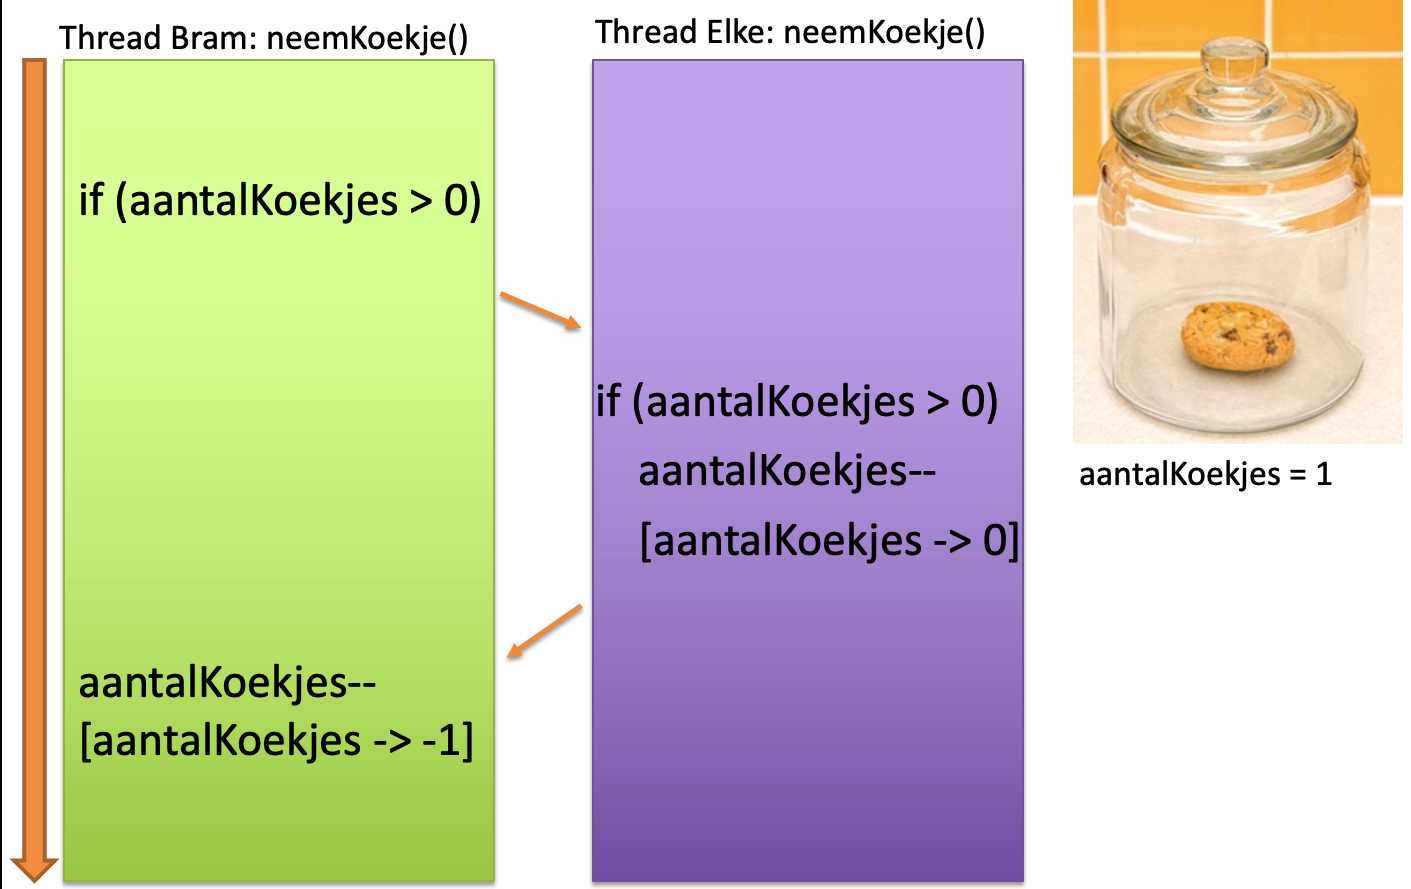
\includegraphics[width=\linewidth]{images/h9/koekjesdoos.png}
  \label{fig:concurrent_access}
\end{figure}

In de bovenstaande afbeelding illustreren we wat er fout loopt.
We verondertstellen dat we 1 processor hebben en dat er 2 threads zijn (Bram en Elke) die gelijktijdig de methode neemKoekje() gaan uitvoeren. Er is nog 1 koekje aanwezig in de koekjesdoos.
Thread Bram is aan de beurt en controleert of er een koekje aanwezig is. Dit is het geval dus de conditie geeft true. Dan beslist de thread scheduler dat de thread Elke  aan de beurt. Deze thread controleert of er nog een koekje is en verlaagt het aantal koekjes met 1. Nu komt de thread Bram terug aan de beurt. De thread hervat zijn werkzaamheden bij het verlagen van het aantal koekjes en nu hebben we dus -1 koekjes. 

Het is dus foutgelopen omdat thread Bram, na de controle of er nog een koekje was, niet direct het koekje heeft ``genomen''.
De koekjesdoos moet dus als het ware beveiligd worden zodat een andere thread niet kan tussenkomen tijdens de uitvoering van de methode ``neemKoekje''.
Programmatorisch kunnen we dit oplossen door de methode neemKoekje() met het keyword \textbf{synchronized} aan te duiden. Dit zorgt als het ware voor een lock (slot) op het Koekjesdoos-object en als \'e\'en thread bezig is een koekje te nemen uit de koekjesdoos, kan een andere thread de koekjesdoos niet afnemen. De andere thread krijgt de koekjesdoos pas als de eerdere thread klaar is met de methode neemKoekje.

\begin{lstlisting}
public class Koekjesdoos {  
     
     private int aantalKoekjes;      
     
     public Koekjesdoos(int aantalKoekjes) {      
         this.aantalKoekjes = aantalKoekjes;   
     }      
     
     public synchronized boolean neemKoekje() {      
         if (aantalKoekjes > 0) {         
             aantalKoekjes--;         
             return true;      
         }     
         return false;  
     }
}
\end{lstlisting}

\subsection{Status WAITING, TIMED\_WAITING en BLOCKED}

\begin{lstlisting}
public class DemoStateBlocked extends Thread {

	private static int value = 0;
	private Thread parent;

	public DemoStateBlocked(Thread parent) {
		this.parent = parent;
	}

	@Override
	public void run() {
		commonResource();
		System.out.println(parent.getState());
	}

	private static synchronized void commonResource() {
		for (int i = 0; i < 100; i++) {
			value++;
			try {
				Thread.sleep(1);
			} catch (InterruptedException e) {
				e.printStackTrace();
			}
		}
		System.out.println(value);
	}

	public static void main(String[] args) throws InterruptedException {
		Thread t1 = new DemoStateBlocked(Thread.currentThread());
		Thread t2 = new DemoStateBlocked(Thread.currentThread());
		t1.start();
		t2.start();
		Thread.sleep(2);
		System.out.printf("%n%s - %s%n", t1.getState(), t2.getState());
		t2.join();
	}
}
\end{lstlisting}

Bovenstaande programma geeft nog eens verschillende thread statussen weer.
Bekijk wat er gebeurt tijdens het uitvoeren van het programma en verklaar de statussen van de verschillende threads.

\begin{verbatim}
TIMED_WAITING - BLOCKED
100
WAITING
200
WAITING
\end{verbatim}

Wat gebeurt er als je de methode commonResource() niet synchronized maakt?

\section{Timer en TimerTask}

De klasse java.util.TimerTask is een abstracte klasse die de Runnable interface implementeert. Je kan deze klasse gebruiken als je een taak op bepaalde momenten wil uitvoeren. 

In de run() methode van een subklasse of instantie van de TimerTask-klasse implementeer je de acties van de taak. In de instantie repeatedTask in onderstaand voorbeeld tonen we de start- en eindtijd van de taak, daartussen wordt er gedurende 2 seconden gewacht.

We gebruiken een object van de klasse Timer om de taak te plannen en te starten.
De Timer-klasse bevat verschillende methodes schedule() om een taak uit te voeren op een gegeven datum of na een bepaalde tijd (delay). Er zijn ook verschillende methodes met de naam scheduleAtFixedRate() waarmee je met een bepaald interval kan herhalen. 

\begin{lstlisting}
import java.time.LocalDateTime;
import java.util.Timer;
import java.util.TimerTask;

public class RepeatTask {

	public static void main(String[] args) {
		TimerTask repeatedTask = new TimerTask() {
			public void run() {
				System.out.println("Task started on " + LocalDateTime.now());
				try {
					Thread.sleep(2000);
				} catch (InterruptedException e) {
					e.printStackTrace();
				}
				System.out.println("Task completed on " + LocalDateTime.now());
			}
		};
		Timer timer = new Timer("Timer");
		long period = 10000L;
		timer.scheduleAtFixedRate(repeatedTask, 0, period);
	}
}
\end{lstlisting}

Als je het bovenstaande programma uitvoert krijg je bijvoorbeeld de volgende output:

\begin{verbatim}
Task started on 2020-12-14T14:50:42.207567
Task completed on 2020-12-14T14:50:44.207988
Task started on 2020-12-14T14:50:52.207359
Task completed on 2020-12-14T14:50:54.209605
\end{verbatim}

De taak wordt iedere 10 seconden (10000 milliseconden) opgestart en zal ongeveer 2 seconden tijd vragen om uitgevoerd te worden.

Wanneer de uitvoertijd van de taak groter is dan de periode tussen opeenvolgende geplande taken, dan worden de taken in een wachtrij geplaatst en zal de volgende taak gestart worden zodra de voorgaande taak is be\"einidigd. Test dit even uit door in het programma RepeatTask de uitvoertijd en de periode tussen de opeenvolgende taken aan te passen.


\section{Concurrency framework}

\subsection{Concurrent collections}

Een groot aantal Collection klassen zijn niet thread-safe. Dit betekent dat ze niet probleemloos door verschillende threads gelijktijdig gebruikt kunnen worden.
Er werd geen concurrency controle voorzien voor de collections om de performatie te maximaliseren in een single-threaded programma.

We illustreren het probleem aan de hand van een voorbeeld. In het onderstaande programma starten we 2 threads die beide 1000 getallen toevoegen in een gemeenschappelijk lijst. Wanneer beide threads klaar zijn, verwacht je dus dat er 2000 getallen in de lijst staan. 

\begin{lstlisting}
import java.util.ArrayList;
import java.util.Collections;
import java.util.List;

public class ConcurrentCollection extends Thread {

	private int id;
	private List<Integer> numbers;

	public ConcurrentCollection(int id, List<Integer> myList) {
		this.id = id;
		this.numbers = myList;
	}

	@Override
	public void run() {
		for (int i =0; i < 1000; i++) {
			numbers.add(id + i);
		}
	}

	public static void main(String[] args) {
			List<Integer> values = new ArrayList<>();
			ConcurrentCollection t1 = new ConcurrentCollection(1000, values);
			ConcurrentCollection t2 = new ConcurrentCollection(10000, values);
			t1.start();
			t2.start();
			try {
				t1.join();
				t2.join();
			} catch (InterruptedException e) {
				e.printStackTrace();
			}

			System.out.println(values.size());

	}

}
\end{lstlisting}

Wanneer we het programma meermaals uitvoeren zien we de volgende getallen als output verschijnen wanneer we het aantal elementen van de lijst opvragen.

\begin{verbatim}
1226
1551
1063
1598
2000
1837
1810
2000
2000
1620
\end{verbatim}


Het kan zelfs gebeuren dat er een exception optreedt.
\begin{verbatim}
Exception in thread "Thread-4" java.lang.ArrayIndexOutOfBoundsException: Index 113 out of bounds for length 109
	at java.base/java.util.ArrayList.add(ArrayList.java:486)
	at java.base/java.util.ArrayList.add(ArrayList.java:498)
	at be.pxl.multithreading.collections.ConcurrentCollection.run(ConcurrentCollection.java:20)
\end{verbatim}

Het probleem is opgelost zodra je een synchronizedList maakt van de lijst values.

\begin{lstlisting}
List<Integer> values = Collections.synchronizedList(new ArrayList<>());
\end{lstlisting}

\subsubsection{Producer-consumer probleem}

Een klassiek synchronisatie-probleem is het producer-consumer probleem (ook gekend als bounded-buffer probleem). Bij het producer-consumer probleem hebben we 2 threads: de producer en de consumer, die beide een gemeenschappelijke buffer met een vaste grootte delen. De producer's taak bestaat uit het genereren van data en deze in de buffer te plaatsen. De consumer verwerkt tegelijkertijd de gegevens die op de buffer verschijnen. Wanneer de buffer vol is, moet de producer even wachten vooraleer hij nieuwe data op de buffer kan plaatsen. Wanneer de buffer leeg is, moet de consumer wachten tot er nieuwe data geproduceerd is.
In de literatuur vind je nog verschillende klassieke synchronisatie-problemen (zoals de dining philosophers) en de problemen die door synchronisatie veroorzaakt kunnen worden (zoals deadlocks), maar deze vallen buiten de scope van deze cursus.

\subsection{Atomic variables}

AtomicInteger is when we are in multi-threaded context and we need to perform atomic operations on an int value without using synchronized keyword.
 
\begin{lstlisting}
import java.util.concurrent.atomic.AtomicInteger;

public class Koekjesdoos {

	private AtomicInteger aantalKoekjes;

	public Koekjesdoos(int aantalKoekjes) {
		this.aantalKoekjes = new AtomicInteger(aantalKoekjes);
	}

	public boolean neemKoekje() {
		int result = aantalKoekjes.getAndDecrement();
		return result > 0;
	}
}
\end{lstlisting}


\subsection{ExecutorService framework}

ExecutorService framework is een API die een hele groep (pool) threads beschikbaar maakt, waaraan je taken kan geven.

Er zijn verschillende factory-methoden beschikbaar om een ExecutorService-object aan te maken. De volgende lijn code toont hoe je een thread-pool met 10 threads kan 
cre\"eeren:

\begin{lstlisting}
ExecutorService executor = Executors.newFixedThreadPool(10);
\end{lstlisting}

Nu kan je een taak toekennen aan de ExecutorService. De ExecutorService kan 2 soorten taken verwerken: Runnable en Callable taken. Callable is een verbeterde versie van Runnable die werd toegevoegd sinds Java 1.5.

Callable$<$V$>$ is een generieke functionele interface  met een methode call() die een waarde van het generieke datatype V teruggeeft als resultaat. 

\subsubsection{Runnable}

\begin{lstlisting}
import java.util.Random;
import java.util.concurrent.ExecutorService;
import java.util.concurrent.Executors;
import java.util.concurrent.Future;

public class ReadFromUrlWithRunnable {

	public static void main(String[] args) {
		ExecutorService executorService = Executors.newFixedThreadPool(5);

		Runnable generateRandomLetters = () -> {
			int leftLimit = 'a'; // letter 'a'
			int rightLimit = 'z'; // letter 'z'
			int targetStringLength = 10;
			Random random = new Random();
			StringBuilder buffer = new StringBuilder(targetStringLength);
			for (int i = 0; i < targetStringLength; i++) {
				int randomLimitedInt = leftLimit + (int) (random.nextFloat() * (rightLimit - leftLimit + 1));
				buffer.append((char) randomLimitedInt);
				try {
					Thread.sleep(1000);
				} catch (InterruptedException e) {
					e.printStackTrace();
				}
			}
			String generatedString = buffer.toString();
			System.out.println(generatedString);

		};
		Future<?> result = executorService.submit(generateRandomLetters);


		System.out.println("Counting down...");
		for (int i = 10; i >= 0; i--) {
			System.out.println(i);
		}
		if (result.isDone()) {
			System.out.println("generating letters is done.");
		} else {
			System.out.println("generating letters is running.");
		}
		executorService.shutdown();
	}

}
\end{lstlisting}


\subsubsection{Callable}

\begin{lstlisting}
import java.io.BufferedReader;
import java.io.InputStreamReader;
import java.net.URL;
import java.util.concurrent.Callable;
import java.util.concurrent.ExecutionException;
import java.util.concurrent.ExecutorService;
import java.util.concurrent.Executors;
import java.util.concurrent.Future;

public class ReadFromUrl {

	public static void main(String[] args) {
		ExecutorService executorService = Executors.newFixedThreadPool(5);

		Callable<String> readData = () -> {
			String urlString = "http://www.google.com";

			// create the url
			URL url = new URL(urlString);

			// open the url stream, wrap it an a few "readers"
			BufferedReader reader = new BufferedReader(new InputStreamReader(url.openStream()));

			// write the output to stdout
			StringBuilder result = new StringBuilder();
			String line;
			while ((line = reader.readLine()) != null) {
				result.append(line).append("\n");
			}

			return result.toString();
		};
		Future<String> data = executorService.submit(readData);
		System.out.println("Counting down...");
		for (int i = 10; i >= 0; i--) {
			System.out.println(i);
		}
		try {
			String bookData = data.get();
			System.out.println(bookData);
		} catch (InterruptedException e) {
			e.printStackTrace();
		} catch (ExecutionException e) {
			e.printStackTrace();
		}
	}

}
\end{lstlisting}


\section{Parallel streams}

Parallelisme is het concept waarbij een probleem wordt opgedeeld in verschillende deelproblemen. Je kan dan verschillende threads aan het werk zetten om voor elk deelprobleem de oplossing te berekenen. Uiteindelijk wordt de oplossing bekomen door de oplossingen van de deelproblemen te combineren. 

In hoofdstuk 7 hebben we geleerd hoe streams gebruikt worden. Het is mogelijk om streams serieel of parallel uit te voeren. Hier is de klasse Employee.

\begin{lstlisting}
public class Employee {
	private String name;
	private int salary;

	public Employee(String name, int salary) {
		this.name = name;
		this.salary = salary;
	}

	public int getSalary() {
		return salary;
	}
}
\end{lstlisting}

Je wil nu weten hoeveel employees een salaris (salary) hebben van 15000 of meer. Ook dit kan je parallel berekenen. Bij de klasse IntStream moet je de methode parallel() gebruiken, bij verzamelingen (collections) gebruik je parallelStream().

\begin{lstlisting}
public class ParallellStreams {

	public static void main(String[] args) {
		List<Employee> employees = new ArrayList<>();
		for (int i = 0; i < 100; i++) {
			employees.add(new Employee("A", 20000));
			employees.add(new Employee("B", 3000));
			employees.add(new Employee("C", 15002));
			employees.add(new Employee("D", 7856));
			employees.add(new Employee("E", 200));
			employees.add(new Employee("F", 50000));
		}
		long t1 = System.currentTimeMillis();

		System.out.println("Sequential Stream Count?= " +
				employees.stream().filter(e -> e.getSalary() >= 15000).count());

		long t2 = System.currentTimeMillis();
		System.out.println("Sequential Stream Time Taken?= " + (t2 - t1) + "\n");
		t1 = System.currentTimeMillis();

		System.out.println("Parallel Stream Count?= " +
				employees.parallelStream().filter(e -> e.getSalary() >= 15000).count());

		t2 = System.currentTimeMillis();
		System.out.println("Parallel Stream Time Taken?= " + (t2 - t1));
	}
}
\end{lstlisting}

Ook hier zie je een snellere uitvoertijd door gebruik te maken van parallellisme.

\begin{verbatim}
Sequential Stream Count?= 300
Sequential Stream Time Taken?= 19

Parallel Stream Count?= 300
Parallel Stream Time Taken?= 8
\end{verbatim}

\section{Oefeningen}

\begin{oefening}
\textbf{Simulatie van het gebruik van een bankrekening}\\
Volgende programma-instellingen worden via properties (programma eigenschappen) beheerd:
\begin{itemize}
\item Startbalans voor een bankrekening
\item Aantal gebruikers die toegang hebben tot de bankrekening
\item Aantal transacties dat iedere gebruiker zal uitvoeren (iedere gebruiker zal evenveel transacties uitvoeren)
\item Limietwaarde voor een transactie (zowel voor geldopneming als storting)
\end{itemize}

Maak nu een bank account aan met de opgegeven startbalans.\\
Maak voor iedere gebruiker een thread aan die het opgegeven aantal transacties zal uitvoeren, dit kunnen zowel geldopnemingen als stortingen zijn. Hou hierbij rekening met de opgegeven limietwaarde. Let wel op dat de balans van bankrekening nooit negatief mag worden.\\
Iedere transactie wordt samen met het resultaat van de transactie weggeschreven in een transaction log bestand.
\end{oefening}

\begin{oefening}
\textbf{Producer-Consumer}\\
Deze applicatie simuleert een productielijn waarop meerdere threads tegelijkertijd en aan een verschillende rate nieuwe producten plaatsen. Een andere thread verwerkt de producten op de lijn aan een bepaalde snelheid. Met de applicatie kan getest worden of de verwerkingsunit de snelheid aankan.
 
\begin{figure}[H]
\includegraphics[width=\linewidth]{images/h9/opgave_producer_consumer.png}
\caption{Producers en consumer}
\label{fig:producer_consumer}
\end{figure}

\textbf{Package}\\
De Package klasse is reeds gegeven, deze bevat enkel een constructor die een ID of volgnummer toekent aan elk nieuw pakketje op de lijn en voorziet ook een toString methode. Hiervoor wordt een klasse variabele gebruikt, deze waarde moet dus niet meegegeven worden bij de creatie van een Package.
\\
\textbf{ProductionLine}\\
Maak een ProductionLine klasse die de productielijn zal voorstellen. Op de productielijn kan je nieuwe producten enkel achteraan toevoegen en enkel vooraan afnemen. Gebruik een verzameling naar keuze uit het Collection framework. Voorzie methoden om een Package toe te voegen aan het einde van de productielijn ( addPackage() ) en om een Package aan de voorkant af te nemen. ( getPackage() ) Denk eraan om de afgenomen pakketjes ook van de productielijn te verwijderen. 
Zorg dat er geen exceptions kunnen optreden als er geen pakketjes meer op de lijn zitten.
Voorzie het nodige om ervoor te zorgen dat alle bewerkingen op de productielijn gesynchroniseerd verlopen en dat het dus niet mogelijk is dat meerdere threads tegelijk een bewerking op de verzameling uitvoeren. (Hiervoor moet je enkel aanpassingen doen op de methoden addPackage() en getPackage() van de ProductionLine klasse.
\\
\textbf{Producer}\\
Maak de Producer klasse aan. Deze zal aan een vast tempo nieuwe Packages aanmaken en deze aan de productielijn toevoegen. De Producer moet kunnen runnen als een thread, dus voorzie daar het nodige voor. In de constructor moet je twee parameters voorzien: de rate waaraan nieuwe producten aangemaakt worden en het productielijn object. De rate is het aantal pakketjes dat deze consumer per minuut aanmaakt.
Wanneer de Producer thread opgestart wordt, moet deze continu nieuwe Packages aanmaken en aan de productielijn toevoegen, met tussenin telkens een pauze zodat de aangegeven rate aangehouden wordt (gebruik hiervoor Thread.sleep(milliseconds)). De thread geeft een korte melding in de console weer, telkens wanneer er een nieuw pakketje op de lijn geplaatst wordt.
Het juiste aantal milliseconden dat de Producer moet wachten tussen 2 pakketjes kan je als volgt berekenen: (60 / rate) * 1000
\\
\textbf{Consumer}\\
De Consumer klasse is gelijkaardig: deze moet ook kunnen runnen als een thread en in de constructor worden eveneens de rate (= opnieuw het aantal pakketjes dat de Consumer per minuut kan verwerken) en het productielijn object meegegeven.
Na opstarten zal de Consumer continu pakketjes van de productielijn afnemen (telkens vooraan) aan de opgegeven rate. Gebruik de methode die je hiervoor voorzien hebt in de ProductionLine klasse. 
De thread print telkens uit welk pakket verwerkt werd. Ook wanneer er geen pakketjes beschikbaar zijn op de productielijn, wordt dit gemeld via een bericht in de console.
\\
\textbf{Main methode}\\
Voorzie tenslotte een main methode. Deze gebruik je om 4 Producers aan te maken met de rates 20, 15, 12 en 7. Daarna maak je ook een Consumer aan met als rate 30. De Consumer verwerkt dus 30 pakketjes per minuut en werkt daarmee sneller dan de 4 Producers. 
Zorg dat al deze componenten correct opgestart worden en parallel hun werk doen. Op deze manier zou je moeten kunnen analyseren of de Consumer voldoende snel werkt om de 4 gelijktijdige Producers aan te kunnen.
\end{oefening}

%---------------------------------------------------------------------------
% Bibliography
%---------------------------------------------------------------------------

%
%\addcontentsline{toc}{chapter}{\textcolor{tssteelblue}{Literature}}
%\printbibliography{}
%

%---------------------------------------------------------------------------
% Index
%---------------------------------------------------------------------------

\printindex

\end{document}
